



\setlength{\overviewextra}{-2pt}
\addtolength{\columnsep}{\overviewextra}
\begin{overview}[-4\baselineskip] %\addcontentsline{toc}{chapter}{Overview}
A substantial change to Australia's tax arrangements is long overdue. The interaction of a fifty per cent capital gains tax (CGT) discount with negative gearing distorts investment decisions, makes housing markets more volatile and reduces home ownership. Like most tax concessions, these tax breaks largely benefit the wealthy.

These two measures in combination allow investors to reduce and defer personal income tax, at an annual cost of \$11~billion to the public purse. Our proposals to wind back the discount and negative gearing would save the Commonwealth Government about \textbf{\$5.4~billion a year}

The discount on capital gains tax is designed to maintain incentives to save and invest.  Because taxes apply to nominal income, inflation would otherwise erode part of an investor's capital gains. Given actual returns, many investors have been overcompensated for inflation. 

Policy has overzealously protected savings at the expense of competing considerations. The economic benefits of tax neutrality for savings are small: those with high incomes save almost the same amount regardless of the tax rate. Providing a discount means that other taxes must be higher, and they impose greater economic costs. The 50 per cent discount also encourages investors to focus too much on investments with capital growth rather than annual income. And it undermines income tax integrity by creating opportunities for artificial transactions to reduce tax.

\textbf{Reducing the capital gains discount to 75~percent} would provide a better balance between these competing considerations and would raise about \textbf{\$3.7~billion} a year.

Negative gearing allows those who borrow to invest to use losses to reduce tax on wages and salaries. In Australia negative gearing goes beyond broadly accepted principles for offsetting losses against gains. It diverts capital from more productive investments without greatly increasing housing supply. Like the CGT discount, negative gearing primarily benefits those on high incomes.

Australia should follow international practice, and not deduct losses from passive investments from wage and salary income.  This change would raise \textbf{\$2~billion} a year in the short term, falling to \textbf{\$1.7~billion} as losses start to be written off against positive investment income. Other proposals, such as restricting negative gearing to new properties or limiting the dollar value of deductions, leave too many problems in place and introduce additional distortions. 

These changes will improve housing affordability -- a little. We estimate housing prices would be up to 2~percent lower than otherwise. Rents won't change much, nor will the rate of new development.  With tight constraints on supply of land suitable for urban housing, most of the impact will be felt via lower land prices. The changes will not cause housing markets to collapse: their effects on prices are small compared to factors such as interest rates and supply of land.

Phasing in change would reduce price shocks and make the reforms easier to sell. It is better than grandfathering current holdings, which would increase complexity, limit the additional tax collected for many years, and be unfair to new investors, especially younger ones.
\end{overview}
\addtolength{\columnsep}{-\overviewextra}
\begin{recommendations}[-35pt]
%\RaggedRight
\raggedright
\begin{enumerate}
\item \textcolor{Orange}{Reduce the capital gains tax discount for individuals and trusts to 75~percent} 
\begin{itemize}
  \item Phase in a 25 per cent discount over ten years through reducing the value of the CGT discount by 2.5 percentage points each year.
\end{itemize}
\item \textcolor{Orange}{Limit negative gearing. Quarantine passive investment losses so they can only be written off against other investment income}
\begin{itemize}
  \item 	Do not allow losses on passive investments to be written off against unrelated labour (wage and salary) income 
\item 	Allow losses on passive investment to be written-off against all current year and future positive investment income, including interest, rental income and capital gains 
\item 	Continue to allow losses from unincorporated business -- sole traders and partnerships -- to be written off against wage and salary income, subject to current restrictions
\item 	Do not create other exceptions -- allowing the write off of losses up to a limit, on one or two properties, or on new properties
\item 	Phase in over ten years by reducing the proportion of losses that can be written off against wage and salary by ten percentage points each year.
\end{itemize}
\pagebreak[2]
\item \textcolor{Orange}{In the longer term, aim to align the tax treatment across different types of savings}
\begin{itemize}
\item	Reduce taxes on other savings income such as net rental income and bank deposits so as to align with the tax treatment of capital gains
\item	Reduce and target the tax incentives for superannuation in line with the recommendations in \Cref{part:SUPER}.
\end{itemize}
\end{enumerate}

\end{recommendations}
%%%
%%%
\chapter{Commonwealth budgets are under pressure}
In five of the last six years, the Commonwealth Government has posted headline deficits of more than 2~per cent of GDP\@.
Assuming revenue and spending projections are correct, Australia is on track for more than a decade of deficits between 2008 and 2019, with Commonwealth net debt projected to peak at 18.5~per cent of GDP in 2017-18,\footcite[][1]{Treasury2015MYEFO201516} higher than any point in the last 45~years.\footnote{Treasury reports Australian Government net debt since 1970-71 \textcite[273]{Treasury2014-MYEFO-2014-15}. Projected debt of 18.5 per cent of GDP is higher than any year reported in the Treasury series, exceeding the previous peak of 18.1 per cent of GDP in 1995-96.}
 
As \Cref{part:FISCAL} highlighted, reaching surplus in the next five years depends on higher income tax collections through bracket creep and optimistic assumptions about economic growth, the terms of trade and spending restraint.
 
The most vulnerable assumption is that growth will return to its long-run trend. The International Monetary Fund recently joined a growing group of economists who believe that long-run economic growth in developed countries including Australia will be slower than in the past.\footnote{The IMF Article IV report on Australia in September 2015 concluded that: ‘Medium-term potential growth is likely to be around 2½ percent rather than the 3¼ percent of the past, bringing per capita GDP growth back to the advanced economy average of around 1 percent’. See: \textcite[][11]{IMF2015b}.}

The government’s fiscal strategy relies heavily on these optimistic projections. But hoping for the best is not a budget management strategy. It simply justifies putting off hard decisions, and shifts the costs and risks of budget repair onto future generations. Our research has previously shown that each year the government runs a \$40\,billion deficit it increases the lifetime tax burden for households headed by a person aged 25 to 34 by \$10,000.\footcite[][9]{DaleyWoodWeidmannEtAl2014}

 
To bring their budgets back to balance, governments will need to undertake reforms on both the revenue and spending sides. History suggests that successful budget repair usually requires simultaneous revenue increases and spending reductions. \footcite[][16]{Daley2013}
 
Over the past two years, the Commonwealth Government has focused publicly on spending cuts to reduce deficits. Ironically, the dominant component of planned budget repair was revenue increase, particularly through fiscal drag. (See \Vref{chapter:FISCAL-1}.) %\footnote{Fiscal drag – growth in income tax collections as a share of wages – accounts for most of the forecast improvement in the budget position between 2015-16 and 2018-19: \textcite{DaleyWood2015FiscalChallenges}, p.~5.}
 
While spending control remains important, some revenue measures could make a meaningful contribution to budget repair with little collateral damage. Recent Grattan papers have shown how governments could improve their fiscal position by targeting superannuation tax concessions, broadening the base or increasing the rate of GST and introducing a broad-based property levy. This report shows that reducing the capital gains tax discount and limiting negative gearing could also make useful contributions.

% \flushcolsend

\chapter{The capital gains discount}\label{chapter:The-capital-gains-discount}
A capital gain is the increase in the value of an asset. Capital gains are taxed when the asset is sold and the gains are realised. The 50~per~cent capital gains tax discount means that the tax rate paid on capital gains is half the rate for other forms of income. 

The purpose of providing a tax discount for capital gains is to reduce the bias income tax creates against savings and investment. But this efficiency benefit needs to be balanced against the costs. 

Tax concessions for capital gains reduce government revenue collections. Other, more distorting taxes, must then be higher. The concessions also distort investment choices because other forms of investment income – such as bank interest – are taxed without discount. Tax concessions for capital gains undermine the integrity of the income tax system by creating opportunities for artificial transactions to reduce income tax. They also reduce the progressivity of the tax system because capital gains are far less evenly distributed than other forms of income. 

Given these costs and benefits, is the capital gains discount set at the right level? While retaining some discount can be justified – primarily because a part of the capital gain is produced by inflation that in principle should not be taxed – the current discount is too generous given the range of competing considerations.


\section{The size and distribution of capital gains}%
\enlargethispage{0.5\baselineskip}%

% cairo pdf for unicode concordance


Australian entities -- individuals, companies, and superannuation funds -- accrued about \$74~billion of income through capital gains in 2013-14. Individuals accrued 45~percent
of capital gains and gained more from real estate than any other source. By contrast, companies and trusts gained relatively little from real estate (\Vref{fig:CGT-by-entity-asset}). Individuals are more likely than institutions to own real estate because progressive state land taxes discourage large property holdings and institutional real estate investment.\FOOTNOTE{See \Cref{part:PROP}. Most institutions invest in commercial property through Real Estate Investment Trusts because company structures do not allow the pass through of tax benefits (such as depreciation allowances).}


\begin{figure}
\captionsetup{margin={0cm,-0.3cm}, oneside, singlelinecheck=false}
\captionwithunits{Individuals earn most capital gains through real estate and shares}{Realised capital gains by source 2013-14, billions}\label{fig:CGT-by-entity-asset}
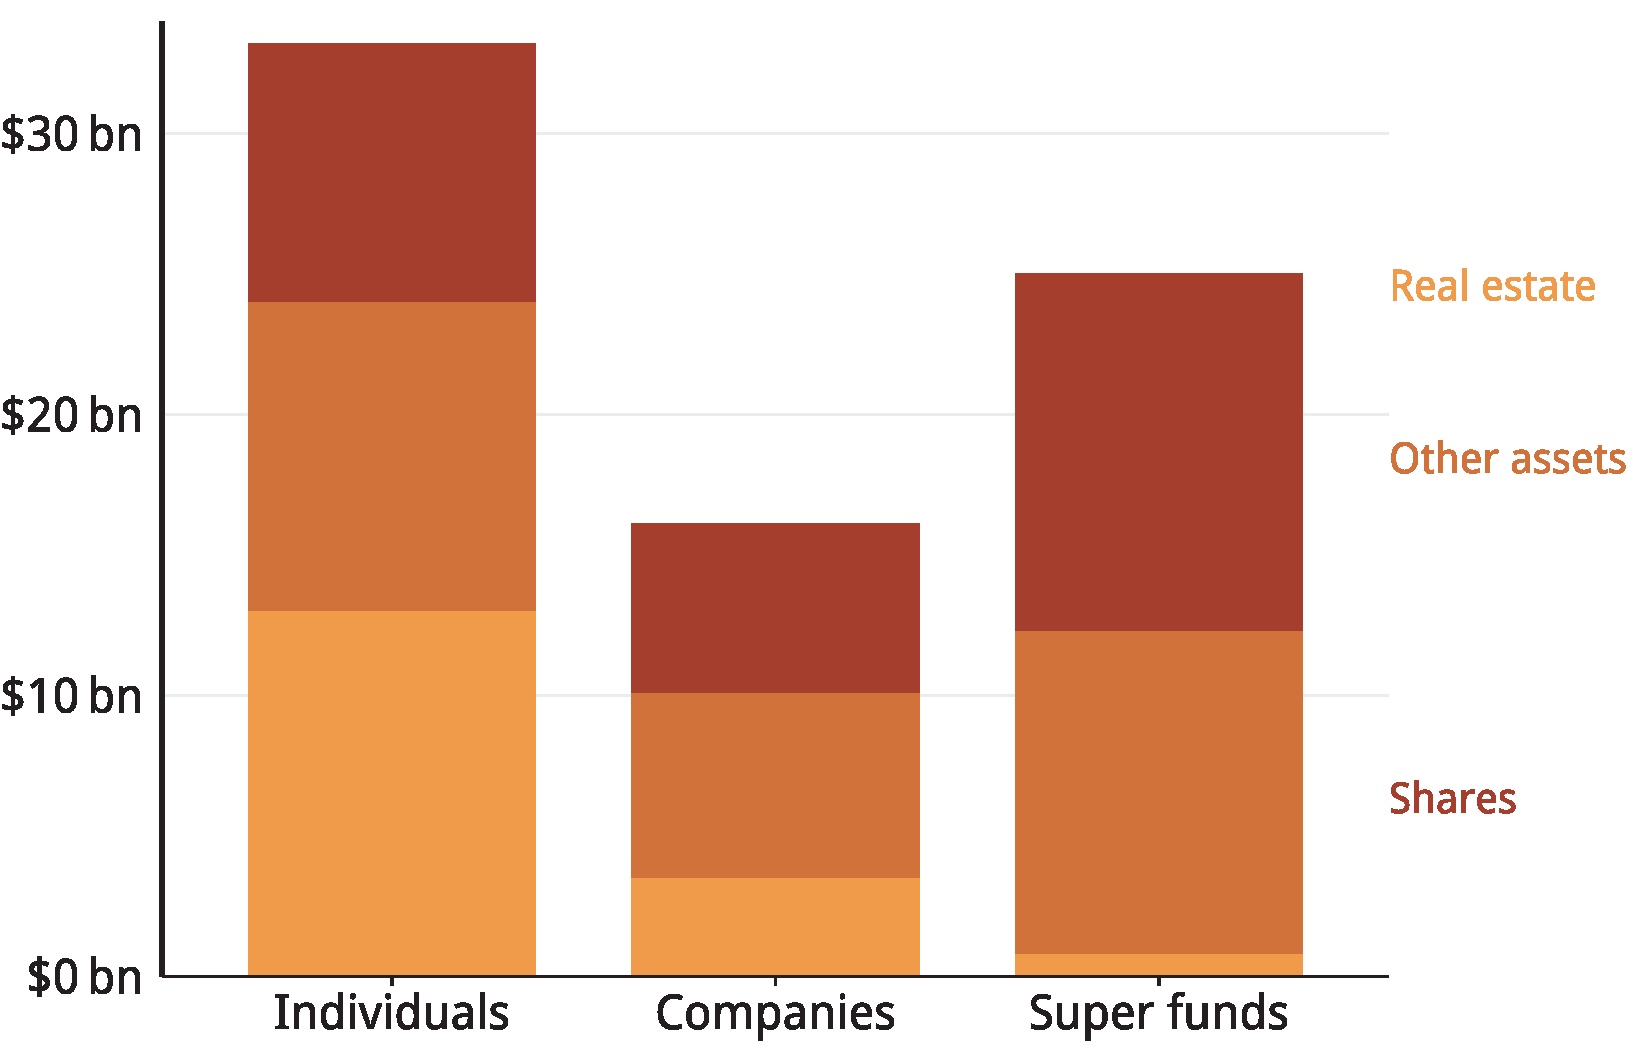
\includegraphics[width=\linewidth]{CGT-NG-atlas/b5-palatino-atlas/CGT-by-asset-1}
\notes{Information is for individuals that completed a CGT schedule. Other assets include business assets and trust distributions that include a capital gain.}

\source{\textcite{ATO2016SampleFile1314}}\par
\vspace*{4\baselineskip}
\end{figure}

These capital gains are taxed as part of the income of individuals, companies and superannuation funds. In 2013-14, capital gains tax raised around \$7.5~billion, around 3~per cent of total income. This is expected to have climbed to \$8.9~billion in the following year.\footnote{2015-16 Budget Paper 1. Table 5 memoranda. \url{http://www.budget.gov.au/2015-16/content/bp1/html/bp1_bs4-03.htm}}

\section{Capital gains receive a range of tax advantages}\label{sec:CG-receive-tax-advantages}
Before 1985, capital gains were not taxed in Australia. Since then, the tax treatment of capital gains has varied, but they have always been taxed at a lower rate than wage and salary income (\Vref{box:Short-History}).%
\enlargethispage{0.5\baselineskip}%

\begin{smallbox}{A short history of capital gains tax changes}{box:Short-History}
Before 1985 capital gains were untaxed in Australia. Taxes on capital gains were introduced to improve the integrity of the tax system, which was undermined by taxpayers recharacterising regular income as capital to avoid tax.\footcite{ReinhardtSteel2006}

Broader taxes on capital gains were introduced to improve the integrity of the tax system, which was undermined by taxpayers reclassifying regular income as capital to avoid tax.\footcites{Evans2005}{Kenny2005} Taxing capital gains in the same ways as other income was also seen as more equitable.\footcite{AustralianGovernment1985}

Between 1985 and 1999, real capital gains (sale proceeds minus the original purchase price adjusted for inflation) were taxed at a taxpayer’s marginal income tax rate. 

As the Ralph Review of Business Taxation recommended, the Howard Government removed indexation adjustments so that tax was applied on nominal gains. To offset the removal of indexation, tax on capital gains income was discounted by 50~per cent for individuals and 33 per cent for superannuation funds for assets held for more than a year. Capital gains of small unincorporated businesses were also discounted by 50~per~cent. 

When this regime was introduced, it was argued that it would stimulate capital markets and make the Australian regime more internationally competitive.\footcite[][14, 598]{RalphReview1999}
\end{smallbox}

For individuals and unincorporated small businesses, 50 per cent of their capital gains on assets held for more than one year are excluded from income. This means the effective tax rate paid on these gains is half the rate applied to other forms of income. Owner-occupied housing is an exception – capital gains on homes are not taxed at all.\footnote{The CGT exemption for the family home is a significant cost to the budget. Changing this policy would have many social and political implications beyond the scope of this report. See: \textcite{DaleyMcGannonSavageEtAl2013BalancingBudgets}, pp.43-45.}

Superannuation funds pay tax on capital gains at 10 per cent (a discount to the 15 per cent they pay on earnings). 

Large corporations pay tax on their capital gains at the corporate rate of 30 per cent, which is the same rate as their income.

Capital gains also receive other less explicit tax advantages compared to recurrent income. First, capital gains are taxed on sale rather than as they accrue. This deferral of tax is akin to the government providing the investor with an interest free loan.  This substantially reduces the effective tax rate paid on gains, with the tax benefit increasing if the asset is held for longer.


With the 50 per cent discount, this deferral over 15 years for a top marginal rate taxpayer reduces the effective nominal tax rate on capital gains from 32 per cent to 28 per cent. (\Vref{fig:CG-marginal-tax-rates-delayed}.)

\begin{figure}
\captionwithunits{The delay in realising capital gains substantially reduces the effective tax rate}%
{Nominal effective marginal tax rates on savings}\label{fig:CG-marginal-tax-rates-delayed}
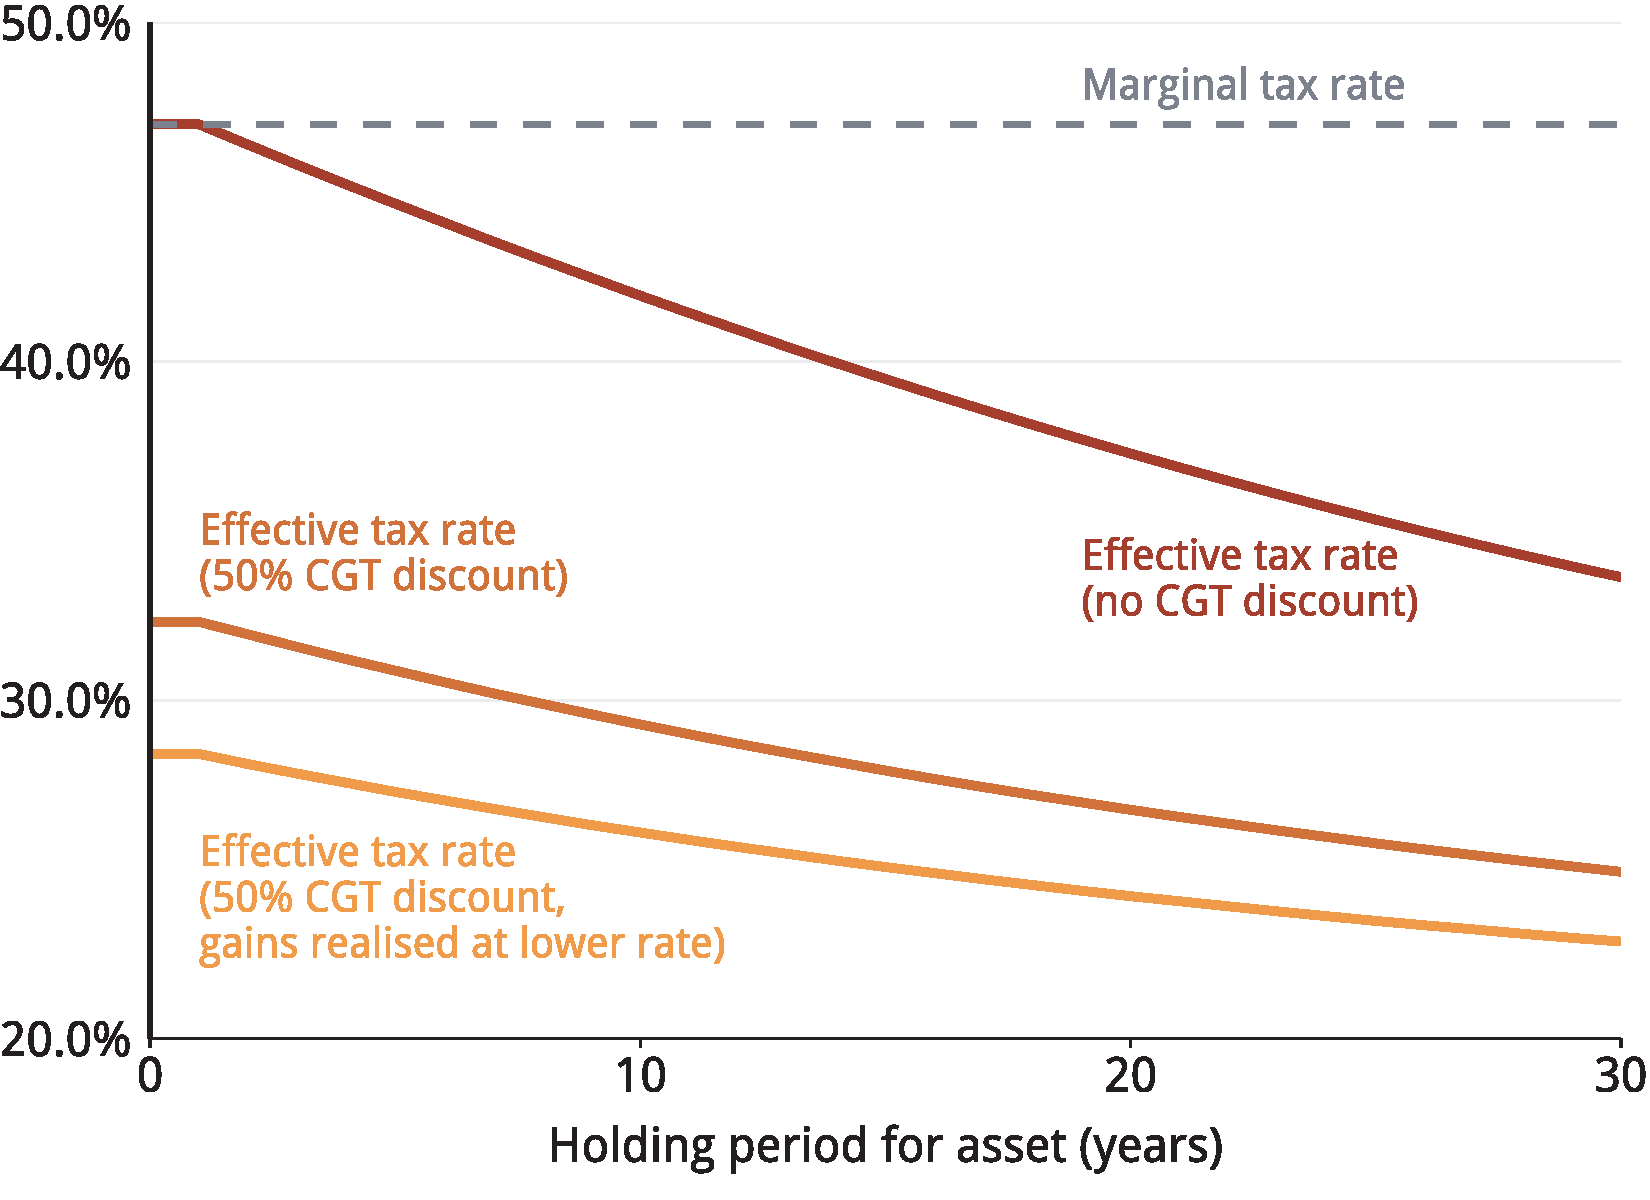
\includegraphics[width=\columnwidth]{CGT-NG-atlas/b5-palatino-atlas/CG-marginal-tax-rates-delayed-1.pdf}
\notes{Assumes 3 per cent nominal income return, 5 per cent nominal capital gain. All returns reinvested to maturity. All gains are realised at investor's nominal tax rate of 47\,c, except final scenario where the investor realises at 34.5\,c marginal rate. Effective tax rate calculated as reduction in annual returns because of tax divided by untaxed~return.}

\source{Grattan analysis}
\end{figure}


Second, investors are also able to choose the time of an asset's sale to minimise taxes on capital gains. They can reduce their tax by selling assets when their income is low, such as after retirement, so they are taxed at a lower marginal rate. 

Some Australians, particularly high income earners, wait until retirement to realise capital gains. Those 65 and older are much more likely to sell assets than those who are younger (\Vref{fig:CGT-by-age-income}).

\begin{figure}
\captionwithunits{Older taxpayers are more likely to have capital gains than younger taxpayers, for all age groups at almost all income levels}{Probability of net capital gains}\label{fig:CGT-by-age-income}
% 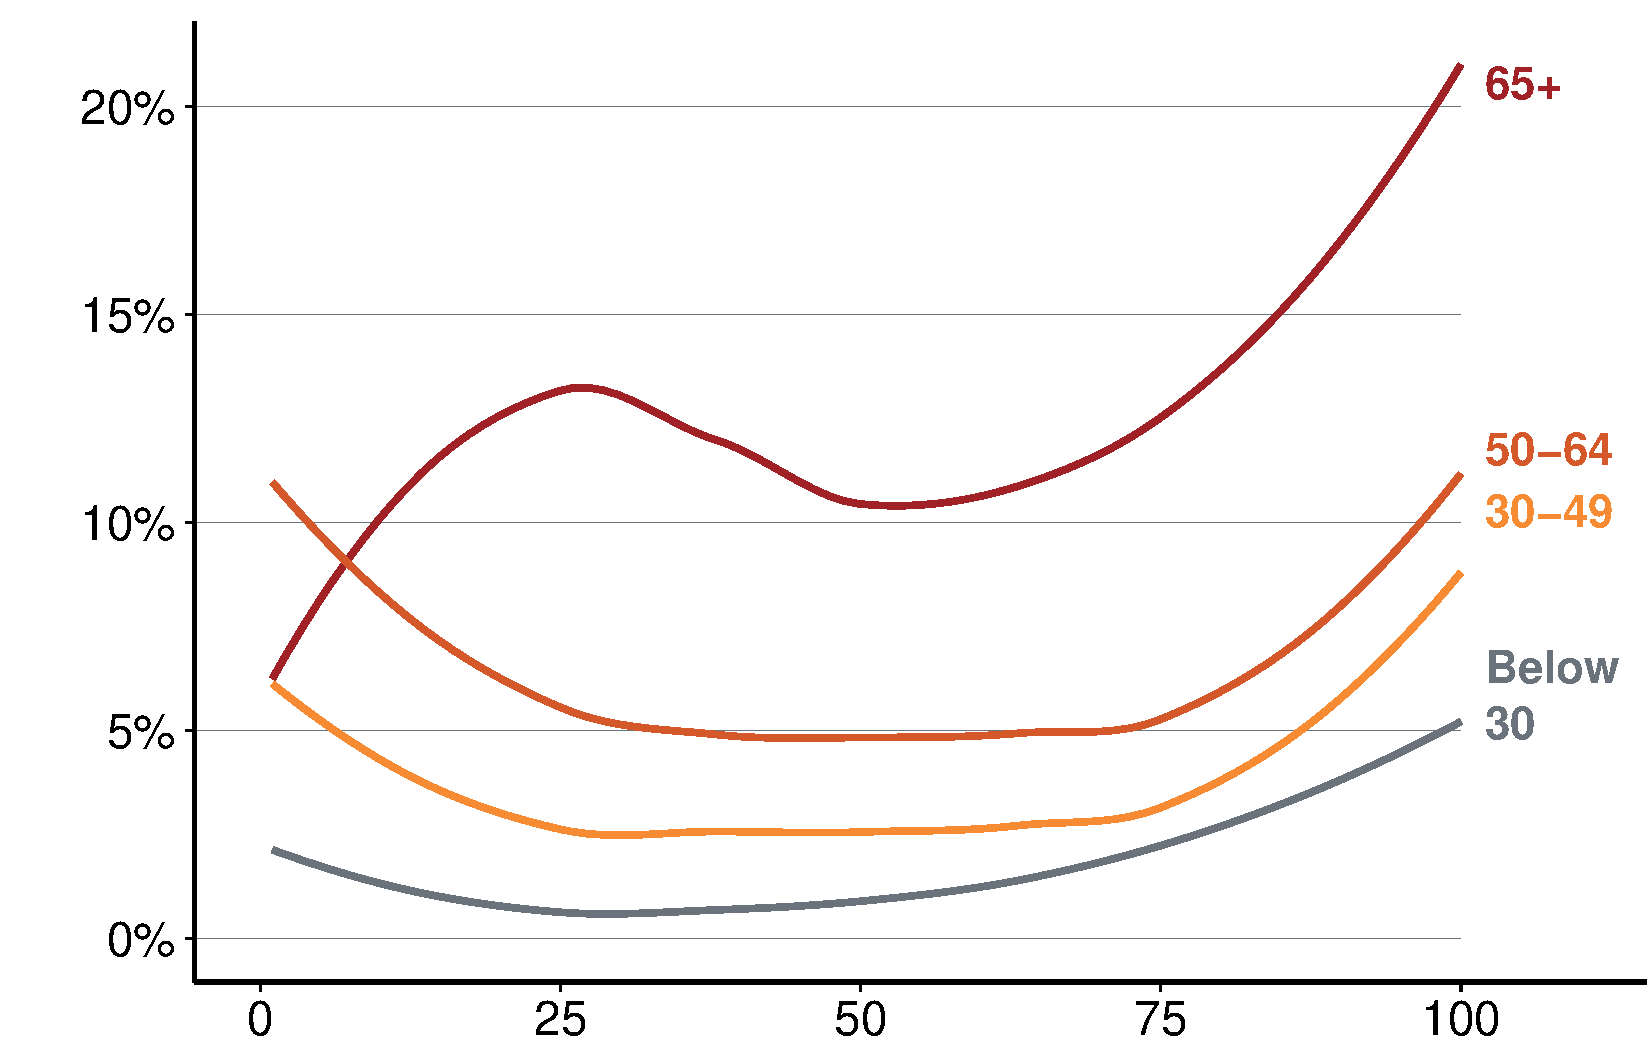
\includegraphics[width=\columnwidth]{CGT-NG-atlas//CGT-by-age-taxable-income-1}
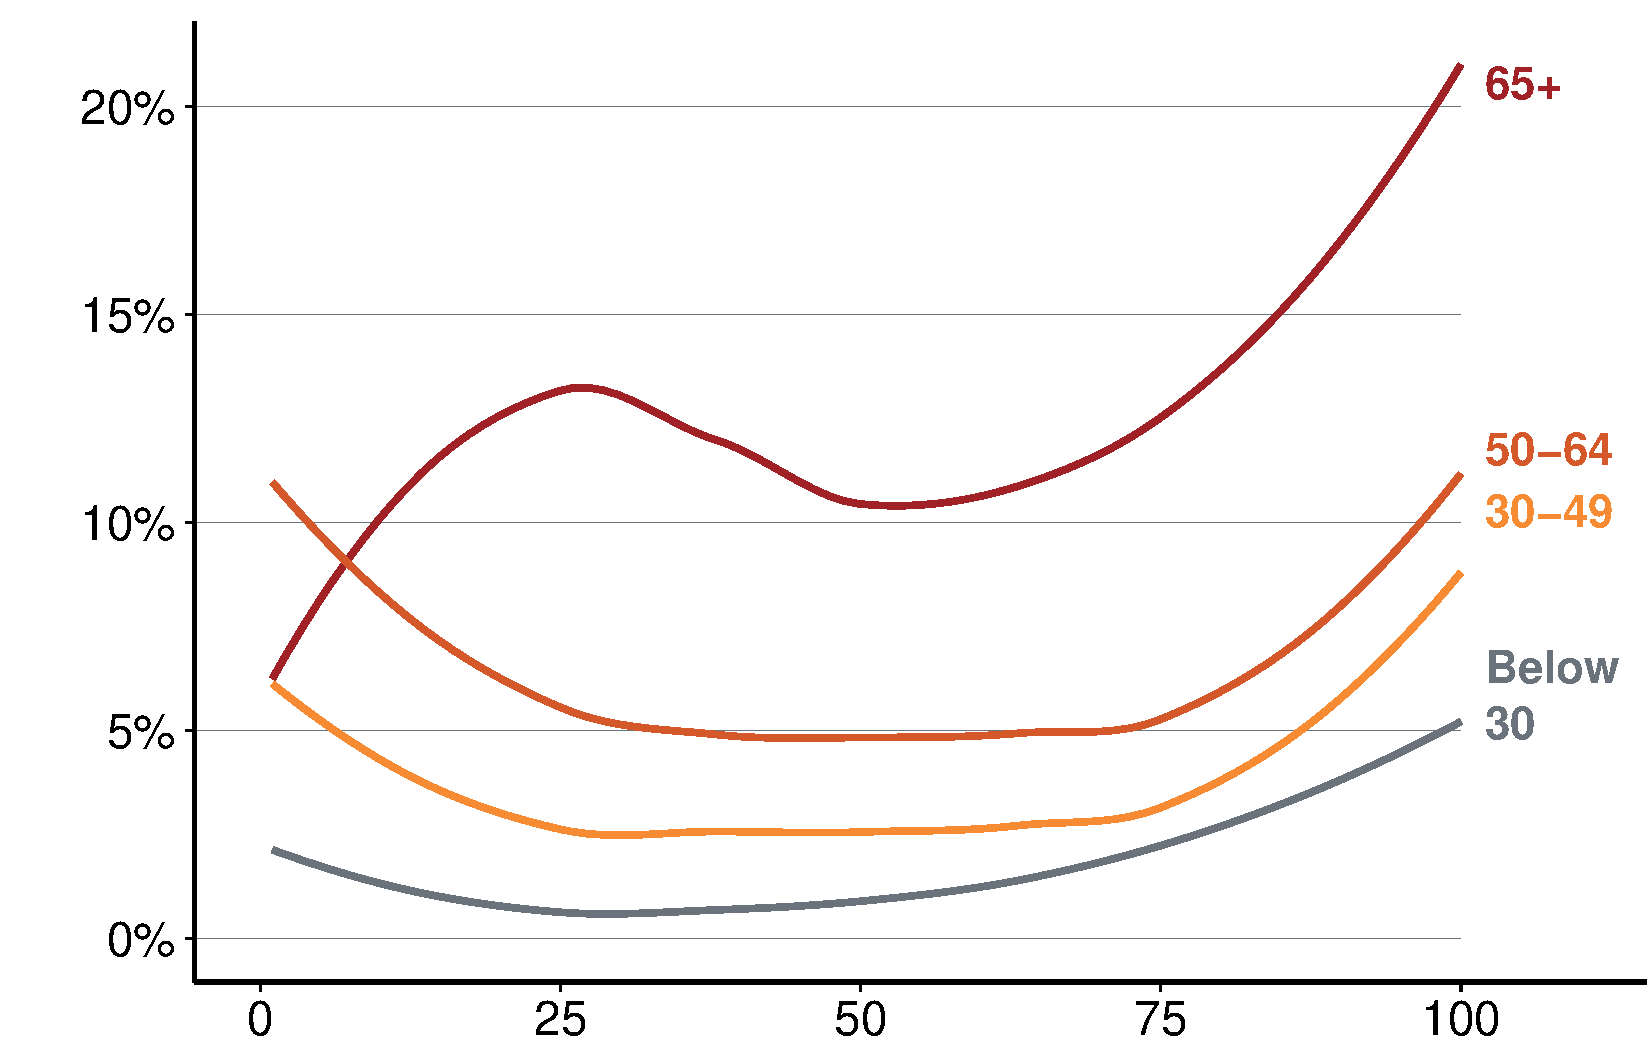
\includegraphics[width=1.1\linewidth]{CGT-NG-atlas/b5-Diana-atlas/CGT-by-age-income-1.pdf}
\end{figure}

The benefits of waiting can be substantial. A person paying the top rate of income tax of 47\,c (including Medicare levy) who times the sale of an investment after 15 years for when they are in the lower tax bracket would reduce the annual nominal tax rate on that investment from 28~per~cent to 25~per~cent. (\Vref{fig:CG-marginal-tax-rates-delayed}.)

The flip side of the benefits to waiting is that taxing capital gains can lead to asset lock-in. Investors are discouraged from selling assets they have held for a long time, even when it would make economic sense to do so,  because they would then pay tax on their accrued gains. More detail is provided in \Vref{appendix:CGT-asset-lock-in}.  


%\FloatBarrier
\section{Some discount is justified to adjust for inflation}
In Australia, taxes on savings income, including capital gains, are levied on nominal returns, which include inflation. Because inflationary gains are not `income' in a true sense,\footnote{They simply offset the loss of purchasing power as price levels increase. See: \textcite[][58]{Treasury2015ReThink}.}  some discount on returns to savings is justified. But the 50 per cent discount has overcompensated property investors for inflation over time. 

A capital gains tax discount is an imperfect adjustment for inflation. The effective tax rate on real returns will depend on both the rate of inflation and the level of returns. (See \Vref{box:tax-on-CG-vary-inflation-returns} and \Vref{appendix:EMTRs}.)

The 50 per cent discount has overcompensated property investors for inflation over the past 15 years. Since the introduction of the capital gains tax discount in 1999, house prices have grown annually by an average of 7.3~per~cent.\footcite{ABS2015HousingFinance} Inflation over this period averaged 2.9~per~cent annually.\footcite{ABSVariousyearsCPI}

In contrast, long-term share investors who experienced low average capital returns because of the global financial crisis would have been better off paying tax on their real capital gains. Share prices have only grown by 3.3 per cent a year since March 2000.\footcite{Finance2015}

Of course, investors in both property and shares received ongoing investment income from rents and dividends that meant their net returns were significantly higher than those from capital gains alone. Indeed, given historical rental yields and capital growth, an investor in the top tax bracket selling a property held for 15 years paid an effective real tax rate of 32~per~cent on their returns, compared to 47~per~cent on their labour income.

Lower future returns would mean somewhat higher effective tax rates. Capital growth for real estate may well be lower in future, as in the last two decades asset prices were boosted by falling interest rates. Interest rates are unlikely to fall much from their current levels, around the lowest in recorded history.\footcite[][19]{Haldane2015}

\begin{smallbox}{Inflation and returns dictate tax rates on real gains}{box:tax-on-CG-vary-inflation-returns}
\addtolength{\parskip}{3pt}
When taxes are levied on nominal returns, as they have been since the capital gains discount was introduced, tax rates on real gains depend on both the inflation rate and the level of returns. 

Consider an investor, Surya, who has \$10,000 worth of shares. The shares pay no dividends so all her returns are through capital growth. The shares increase in value by 8 per cent over the first year while inflation is 2.5 per cent. If she were to sell the shares at the end of the year her nominal return would be \$800. Her real (inflation-adjusted) return is \$540. 

If she paid \textbf{tax directly on her real gain} at the 47 per cent top marginal tax rate, she would pay \$252 in tax. So her \textbf{real after-tax return would be \$288}. If instead she \textbf{paid tax on her nominal gains that had been discounted by 50 per cent} then she would pay tax of \$188 (47 per cent tax on half her nominal gains of \$800) and thus receive a \textbf{real after-tax return of \$352} (\ie, her real return of \$540 minus the \$188 tax). Therefore, in this scenario with returns at 8 per cent and inflation at 2.5 per cent, she is much better off being taxed on her nominal gain with the 50 per cent discount than being taxed directly on her real gains. 

However, the opposite is true if returns are low. If Surya’s shares only increase in value by 3 per cent annually, her nominal return would be \$300 and her real (adjusted for inflation) return would be \$49. If she paid tax on real gains her tax would be \$23 and she would make \textbf{real after tax returns of \$26}. In contrast, if she is taxed on 50 per cent of her nominal gains she pays tax of \$70 and makes a \textbf{real after tax loss of \$22}.
\end{smallbox}



\section{What is the `right' tax rate on capital gains?}\label{sec:What-is-the-right-tax-rate-on-capital-gains}
Beyond compensating for the effects of inflation, the right tax rate for earnings on savings, and capital gains in particular, depends on a range of competing considerations. 

In an ideal taxation world, taxes on savings should leave investors neutral between consuming today and consuming tomorrow. In other words, no investor should be penalised for saving. To achieve this ideal, there should be no tax on the component of savings returns known as ‘returns to waiting’, or the ‘risk-free rate’.\footnote{This chapter discusses the nominal risk-free rate, which compensates for both inflation and waiting. In Australia the 5 year government bond rate – a proxy for the risk-free rate – has averaged around 2.8 percentage points above the inflation rate over the past 25 years. \textcite{RBA2015CapitalMarketYields}.} This component of returns is not reward for risk-taking or skill but simply for forgoing access to money for a period. 

The right tax rate on savings could be even lower if governments are seeking to promote entrepreneurship through the tax system.
On the other hand, there are good reasons to impose taxes on capital gains higher than this theoretical ideal.

First, all societies need taxes, all taxes impose costs, and the cost of taxes on savings must be balanced against the economic cost of raising revenue through other taxes. Taxes on savings are more economically desirable than many other taxes because they don’t have much effect on behaviour. People who can afford to save will tend to do so regardless of the tax rate.

Second, higher taxes on capital gains reduce the incentives for tax avoidance: taxpayers structuring transactions so that earnings are re-classified as capital gains to attract the lower tax rate.

Third, higher taxes on capital gains reduce distortions in investment choices. Other forms of investment income – such as bank interest – do not receive concessional tax treatment. 

Finally, higher taxes on savings, and capital gains in particular, limit growth in inequality. Higher taxes on capital gains can act as de facto wealth taxes.  

The next two sections discuss the considerations for and against maintaining the current concessional tax treatment of capital gains in more detail.


\section{Arguments for maintaining a significant tax concession for capital gains}
\subsection{Not distorting decisions between consumption today and saving for tomorrow}
Taxes on income from savings, including capital gains, reduce incentives to save.\footcites[][32]{HenryTaxReview2010}[][58]{Treasury2015ReThink}[][295]{MirrleesAdamBesleyEtAl2011}  In effect, taxes on returns to savings make future consumption more expensive relative to current consumption, so people have incentives to consume more and save less. Taxes on savings also somewhat reduce the incentives to work today, by lowering the payoff from working to save for the future.\footcite[][12]{HenryTaxReview2010}  In the theoretical ideal, taxes would leave people neutral between consumption today and consumption tomorrow.

Although economists do not all agree, many proponents of ‘optimal tax theory’ – including the Mirrlees tax review in the UK  – advance the view that the way to achieve this neutrality is to not levy tax on the risk-free returns to savings (\Vref{box:RiskFreeReturns}).\footnote{\textcite[][284]{MirrleesAdamBesleyEtAl2011}. See also the sources cited \textcite[][2]{Ingles2015}. Others such as \textcite[][1]{Carling2015} suggest the optimal tax rate on capital gains may be zero.} 
Others such as \textcite{BanksDiamond2008}\DEVIATION{} % correct 
conclude that it may still be optimal to tax the risk-free return to savings, albeit at a lower tax rate than other income.%
\footnote{This is because \textcite{BanksDiamond2008} also consider progressivity: they point out that those with higher earning capacity (generally higher levels of education) tend to have greater ability and willingness to smooth consumption over their lifetime, while those with lower earning capacity tend to be more uncertain about their future lifetime earnings.}  

\begin{smallbox}[tbp]{What are risk-free returns?}{box:RiskFreeReturns}
One component of returns to savings is the risk-free rate. Most people prefer to have a thing today rather than acquiring the same thing tomorrow. So people need to receive some compensation for deferring consumption. Of course, different people may care more or less about waiting: those on lower incomes tend to put more of a premium on immediate consumption than those on higher incomes.   The (nominal) risk-free rate also includes compensation for inflation – increases in the general price level that erode purchasing power. 

The average cost of waiting is often described in finance as the ‘risk free’ rate. The proxy used to measure this rate is the interest rate paid on government debt where there is minimal risk of default, and the investor only gets a return for waiting. 
\end{smallbox}

The corollary of exempting the risk free returns from tax is that what are known as ‘excess returns’ – the other component of returns to savings – should be taxed.%
\footnote{Excess returns are defined broadly to include the investment risk premium (required to compensate the investor for uncertain returns), economic profits (returns due to unique skill, idea or patent) and supernormal returns (higher returns from good luck). See: \textcite[][153]{PresidentsAdvisoryPanelTaxReform2005Proposals}.}

For property investors paying tax at the top marginal rate, the current capital gains tax regime has taxed their excess returns at almost the same effective rate as income over the past 15 years, as shown in \Vref{fig:EMTR-savings}. In other words, the current regime has delivered results very close to the theoretical ideal for those that held assets over the period. 

But that may not last. The effective tax rate on excess returns will vary with total returns, inflation, and changes in the risk-free rate. If investment returns are lower in the future, then effective tax rates on excess returns would be higher than over the last 15 years (\Vref{fig:EMTR-savings}), and might deter saving to some extent. 

\begin{figure}[!tp]
\captionwithunits{The effective tax rate on excess returns for property has been close the income tax rate over the past 15 years}{Effective marginal tax rates on savings}\label{fig:EMTR-savings}
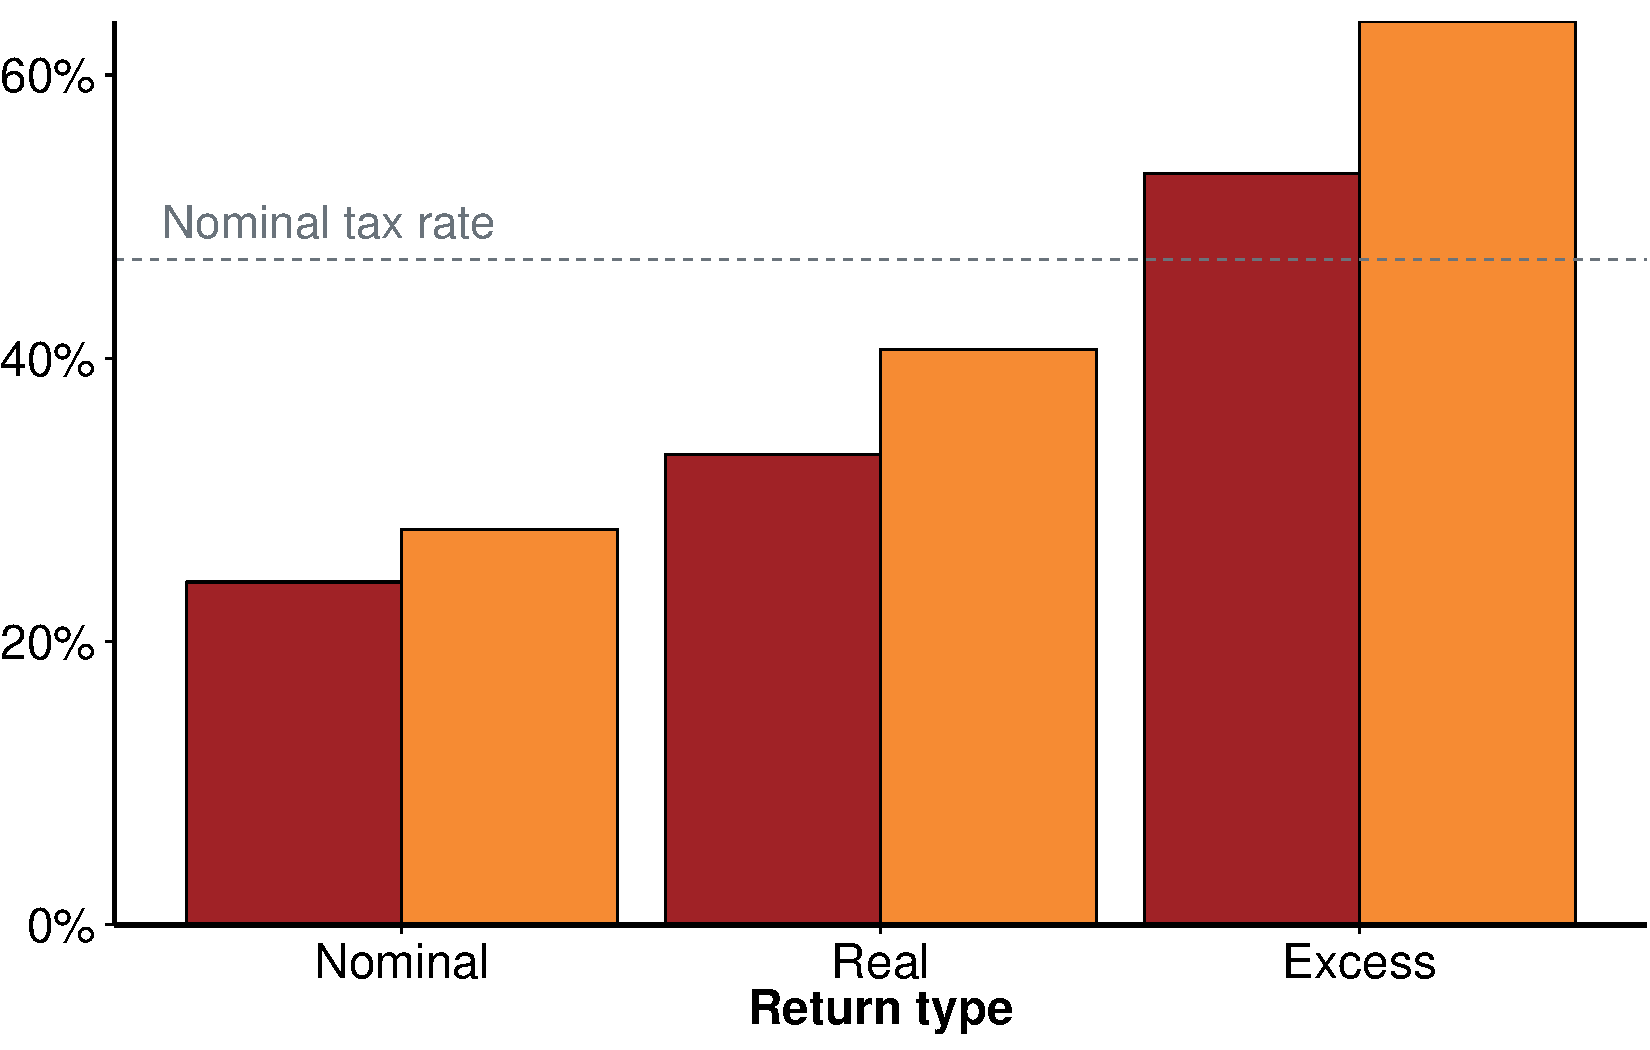
\includegraphics[width=\columnwidth]{CGT-NG-atlas//EMTR-nominal-real-excess-historic-vs-lower-1}
\fnotes{fig:EMTR-savings}{Assumes: marginal tax rate of 47\%, property held for 15 years, nominal rent at 3\% of the property value. 

\begin{table}
\centering
\captionsetup{justification=centering}
\caption{Assumptions for \Vref{fig:EMTR-savings}}\label{tbl:EMTR-savings-assumptions}
% latex table generated in R 3.2.5 by xtable 1.8-2 package
% Sun Apr 24 12:04:28 2016
\footnotesize
\begin{tabular}{llrrr}
  \toprule
   &  &  &  &  \\
 \textbf{return type} & \textbf{scenario} & \textbf{capital gains} & \textbf{risk free rate} & \textbf{inflation} \\
 \midrule
excess & historic & 7.3\% & 5.6\% & 2.8\% \\ 
  excess & lower & 5.0\% & 4.5\% & 2.5\% \\[4pt] 
  nominal & historic & 7.3\% & 5.6\% & 2.8\%\\ 
  nominal & lower & 5.0\% & 4.5\% & 2.5\%  \\[4pt] 
  real & historic & 7.3\% & 5.6\% & 2.8\%  \\ 
  real & lower & 5.0\% & 4.5\% & 2.5\%  \\ 
   \bottomrule
\end{tabular}

\end{table}
}

\source{Grattan analysis}
\end{figure}

On the other hand, the theoretical ideal implicitly assumes losses and gains are taxed symmetrically. But this is not the case. Capital gains are taxed on realisation and at the time of the investors’ choosing (\Cref{sec:CG-receive-tax-advantages}) whereas losses can be written off against taxable income each year. As we show in \Cref{chapter:Impacts}, this means that effective tax rates are lower for negatively geared investments than for investments fully financed from savings as is assumed in \Vref{fig:EMTR-savings}. Effective tax rates for investors under a range of alternative return scenarios and tax rates are summarised in \Cref{appendix:EMTRs}.%
\footnote{\textcite{GreenMyersonLichtmanEtAl1996} demonstrate older low income adults have much higher discount rates (\ie they put more value on consumption today rather than in the future) than higher income adults of all ages. Others have also identified that those on lower incomes have higher discount rates:  \textcites{ReimersMaylorStewartEtAl2009}{HarrisonLauWilliams2002}.}

\subsection{Maintaining incentives for risk-taking and entrepreneurship}\label{subsubsec:maintain-incentives-for-risk-taking}
A tax discount for capital gains is also sometimes justified on the basis that taxing capital gains will deter entrepreneurship and risk taking by reducing the returns to selling a successful business.\footnote{\textcite[][8--11]{ClemensLammamLo2014}. If capital gains were taxed on an accrual basis and capital losses were fully tax refundable, then taxing gains in full would be neutral with respect to risk. However, since losses are only deductible against gains, investors risk making a loss they will not able to deduct. It is not clear whether deferral of taxes on gains until realisation, itself a significant tax advantage (Section 2.2), is itself enough to compensate investors for this risk. \textcites[8]{Burman2009}[130]{ProductivityCommission2004FirstHomeOwnership}.} 
But this effect is unlikely to be large. Other factors that influence entrepreneurship and risk-taking behaviour are far more significant to returns than the tax on any gains ultimately made.\footcite[][75]{Burman1999} 

One plausible reason for taxing excess returns at the same rate as income is that taxes on risk-taking should be similar to taxes on working. Obviously there need to be some rewards to taking risks. But on the other hand, why should the after-tax returns to risk-taking be higher than the after-tax returns to working? 

Some argue that capital tends to be more mobile than labour, and so should be taxed less to keep it from moving. Yet taxes on savings by individuals are generally levied where the individual lives, rather than where the capital is invested. Investors are not that much more mobile than workers.

In any case, most capital gains for individuals are from property and sharemarket investments (\Vref{fig:CGT-by-entity-asset}). Specific small business exemptions are a far more targeted way to address any tax disincentive for entrepreneurial effort. A number of other exemptions are already in place to limit the effects of capital gains tax when assets or businesses are sold (\Vref{box:small-biz-cgt-exemptions}). It is arguable that these are overgenerous. 

\begin{smallbox}{Small business capital gains tax exemptions}{box:small-biz-cgt-exemptions}
Small business owners enjoy a range of generous exemptions from capital gains tax.  
They can receive exemptions for the sale of active assets up to a lifetime limit of \$500,000. For those under 55, the proceeds must be paid into a complying super fund to receive the exemption (‘retirement exemption’). 

There are also CGT exemptions for people over 55 that are retiring and selling business assets held for more than 15 years (the ‘15\nobreakdash-year exemption’). A lifetime cap of \$1.395 million applies to the retirement exemption and the 15-year exemption. 

Small business owners also receive rollover relief, allowing them to defer all or part of a capital gain for two years or longer on the sale of active assets, provided they acquire a replacement asset or make capital improvements to an existing asset.

In its recent innovation statement, the Government announced further capital gains tax relief for investors in start-ups. Investors receive a ten-year exemption from capital gains tax so long as they hold the investment for at least three years.

Given this raft of concessions, it has been described as a ‘mystery’ that small business ever pays any capital gains tax.

\source{\textcites{ATO2014f}{Government2015NationalScienceInnovationAgenda}[][6]{Ingles2015}}
\end{smallbox}


\section{Arguments for lower tax concessions for capital gains}\label{subsec:arguments-lower-tax-concessions-for-capital-gains}

The ‘optimal’ tax on savings discussed in the previous section assumes that the only considerations are achieving neutrality between savings and immediate consumption.

Yet of course other considerations exist. Indeed, it is not obvious that the trade-off between savings and immediate consumption should even be the \emph{primary} consideration for setting taxes on savings, apart from the relative ease with which it can be modelled.
\subsection{Balancing the costs of other taxes}
If savings taxes are lower, then other taxes need to be higher than otherwise. Inevitably these taxes impose costs of their own – all taxes distort behaviour from an untaxed ideal. So \emph{how much} savings taxes distort behaviour must be compared with the size of distortions due to other taxes that would otherwise be higher.

In fact, taxes on savings probably do not do much to distort total savings from ideal levels. Savings behaviour is relatively unresponsive to tax rates.\footnote{Optimal taxation requires that commodities should be taxed at rates inversely related to their demand elasticities. So if demand for future consumption is relatively inelastic, an efficient tax system would more heavily tax saving activity. \textcite[See:][21--22]{Ingles2015}.}  Empirical evidence mainly suggests that changes in tax rates affect investors’ choice of investment much more than the total amount saved. This is particularly the case for those on high incomes, who tend to save the most.\FOOTNOTE{See \textcite[][59]{Treasury2015ReThink} as well as \Vref{sec:SUPER-2-6} for a summary of the literature on the impact of tax concessions on retirement savings efforts. While most studies look at tax concessions for retirement savings, a review of the experience of tax-preferred savings accounts in 11 OECD member countries also suggests that high-income people are most likely to participate in tax preferred savings plans but tax preferred accounts only create new savings when people of moderate incomes participate in them. See: \textcite[][]{OECD2007EncourageSavingsThroughTaxPreferredAccounts}.}

By contrast, the \emph{actual} distortions due to other taxes may be quite high. For example, for middle-income women with children, take home pay can be very low after paying income tax and giving up welfare and paying for childcare. These costs substantially reduce workforce participation.\footcite[44--47]{DaleyMcGannonGinnivan2012}

\subsection{Reducing distortion between investment choices}\label{subsubsec:reducing-distortion-between-investment-choices}
Providing a tax discount for capital gains but not for other investment income does distorts where people choose to invest. 

Capital gains have substantial tax advantages relative to annual earnings. The capital gains discount magnifies the tax advantages because capital gains are not taxed until they are realised (\Vref{fig:CG-marginal-tax-rates-delayed}). In contrast, Australia’s current tax system does not adjust for the effects of inflation on bank deposits, which are assets disproportionately held by the least well off.\footnote{Bank deposits comprise 20 per cent of the assets of the households in the lowest income decile compared with around 5 per cent for the top two income deciles (\textcite{HILDA2015}).}  Rental income, bond yields and returns from overseas shares are also taxed at full marginal rates. 

Taxing capital gains more lightly than most other savings income creates an incentive for investors to choose riskier assets that return more via capital gain. In conjunction with generous rules for deductibility of interest costs, the tax system creates strong incentives for debt-financed and speculative investments (\Cref{sec:negative-gearing-provides-a-widely-used-tax-shelter-on-wages}). As a result, Australians invest more in property and less in bank deposits than economic fundamentals would suggest is ideal.

The efficiency losses generated by the different tax treatment of different forms of savings are likely to be much larger than from the weight of taxes on capital in general.\footcites[][16]{Ingles2009TaxEquity}[][22]{Ingles2015}  Of course, the economic cost of differing tax treatments is also an argument for taxing savings earnings less rather than taxing capital gains more. But substantial budget deficits leave little room to reduce taxes on other forms of savings income. Consequently, the most plausible way in practice to reduce the distortions between different forms of savings is to increase the taxes on capital gains \Vref{sec:Impact-new-development}. 

However, increasing taxes on capital gains will increase the incentives to invest in owner-occupied properties and in superannuation, which already enjoy even larger tax concessions than capital gains. People would be encouraged to invest even more in their principal residence, by renovating, and purchasing bigger and better-located homes. 

There is some truth to these concerns, but they shouldn’t be overstated. 

First, there is at least a plausible rationale\label{subsubsect:plausible-rational-for-encouraging-investment-in-owner-occupied-housing}
 for encouraging additional investment in owner-occupied housing,\footcite[][43--45]{DaleyMcGannonSavageEtAl2013BalancingBudgets} the biggest single component of wealth.\footnote{Owner-occupied housing (net of property loans) is almost 40 per cent of the net worth of Australian households. \textcite[See:][]{ABS2015HousingFinance}.} Governments have deliberately promoted home ownership because of the social benefits including enforced savings, social stability and community involvement.\footnote{The tax-free status of the family home is so entrenched that a recent inquiry into the Tax Expenditure Statement recommended it be removed as a tax expenditure, arguing that it now so unquestioned it is in effect the benchmark tax treatment for this asset. \textcite[][42]{HouseOfRepresentativesStandingCommitteeonTaxRevenue2015TES}.} Therefore, further widening the tax advantage for owner-occupied housing by reducing the CGT discount may not necessarily be a net social cost.\footnote{The Henry Tax Review recommended that long term lifetime savings through owner-occupier housing continue to remain exempt from tax because of these benefits \textcite[][Part A, p.~4]{HenryTaxReview2010}).}


While some tax incentives for superannuation might be justified, the current regime is too generous and poorly targeted. Grattan Institute’s 2015 report, \textit{Super tax targeting}, argues that they should be wound back.\FOOTNOTE{See \cpageref{overview:SUPER} in \Cref{part:SUPER}.} %\footcite[][1]{DaleyCoatesWoodEtAl2015Super} 
In the meantime, failure to reform superannuation should not hold back capital gains tax reform. 

Second, reducing the discount might not lead to much greater investment in owner-occupied housing and superannuation. Households already hold 40 per cent of their assets outside these areas, even though they give up substantial tax advantages.\footcite{ABS2015HousingFinance} This is presumably because people want savings in forms that are available for use before retirement and without having to sell their home.  


\subsection{Maintaining the integrity of income tax collections}
Tax concessions for capital gains can increase ‘revenue leakage’ as taxpayers convert what many people would intuitively view as labour income into capital gains, in order to pay less tax.\footcites{Evans2005}{MinasLim2013} Protecting the income tax base is a key reason for taxing capital gains in most OECD countries\footcite{OECD2006TaxationOfCapitalGains}  and prompted the introduction of a general capital gains tax in Australia in 1985 (\Vref{box:Short-History}). 

Traditionally, this type of tax shelter has been the preserve of the wealthy. Examples include paying executives with shares or stock options,\footcite[][8--9]{Ingles2009TaxEquity} and reorganising private corporations to convert dividend income into capital gains.\footcite{MinasLim2013} Negative gearing (discussed in Chapter 3) effectively converts wage income into more concessionally taxed capital gains (\Cref{sec:negative-gearing-provides-a-widely-used-tax-shelter-on-wages}).  

\subsection{Maintaining the progressivity of the tax system}\label{subsec:maintaining-progressivity-tax-system}
If returns to savings are not taxed, inequality will almost certainly widen. The top ten per cent of wage and salary earners receive about a third of all wages and salaries (before tax). They tend to save a greater proportion of their income than people who earn less.\footnote{The top 20 per cent of households by disposable income save on average 35 per cent of their disposable income. This compares to dissavings of 25 per cent for the lowest income quintile and savings rates of less than 10 per cent for the second and third quintiles. \textcite[][table~5]{ABS2014DistributionHouseholdIncome}.} And they are more likely to invest in higher risk and return assets, including assets where a higher proportion of the total returns are from capital gains. Indeed, as \Vref{fig:CG-by-decile} shows, the top ten per cent of individual income earners received 55 per cent of all investment income, and 67 per cent of all capital gains income. 

\begin{figure}[!ht]
\captionwithunits{Most capital gains are earned by those in the highest income decile}{Proportion of net capital gains by income decile (2013-14)}\label{fig:CG-by-decile}

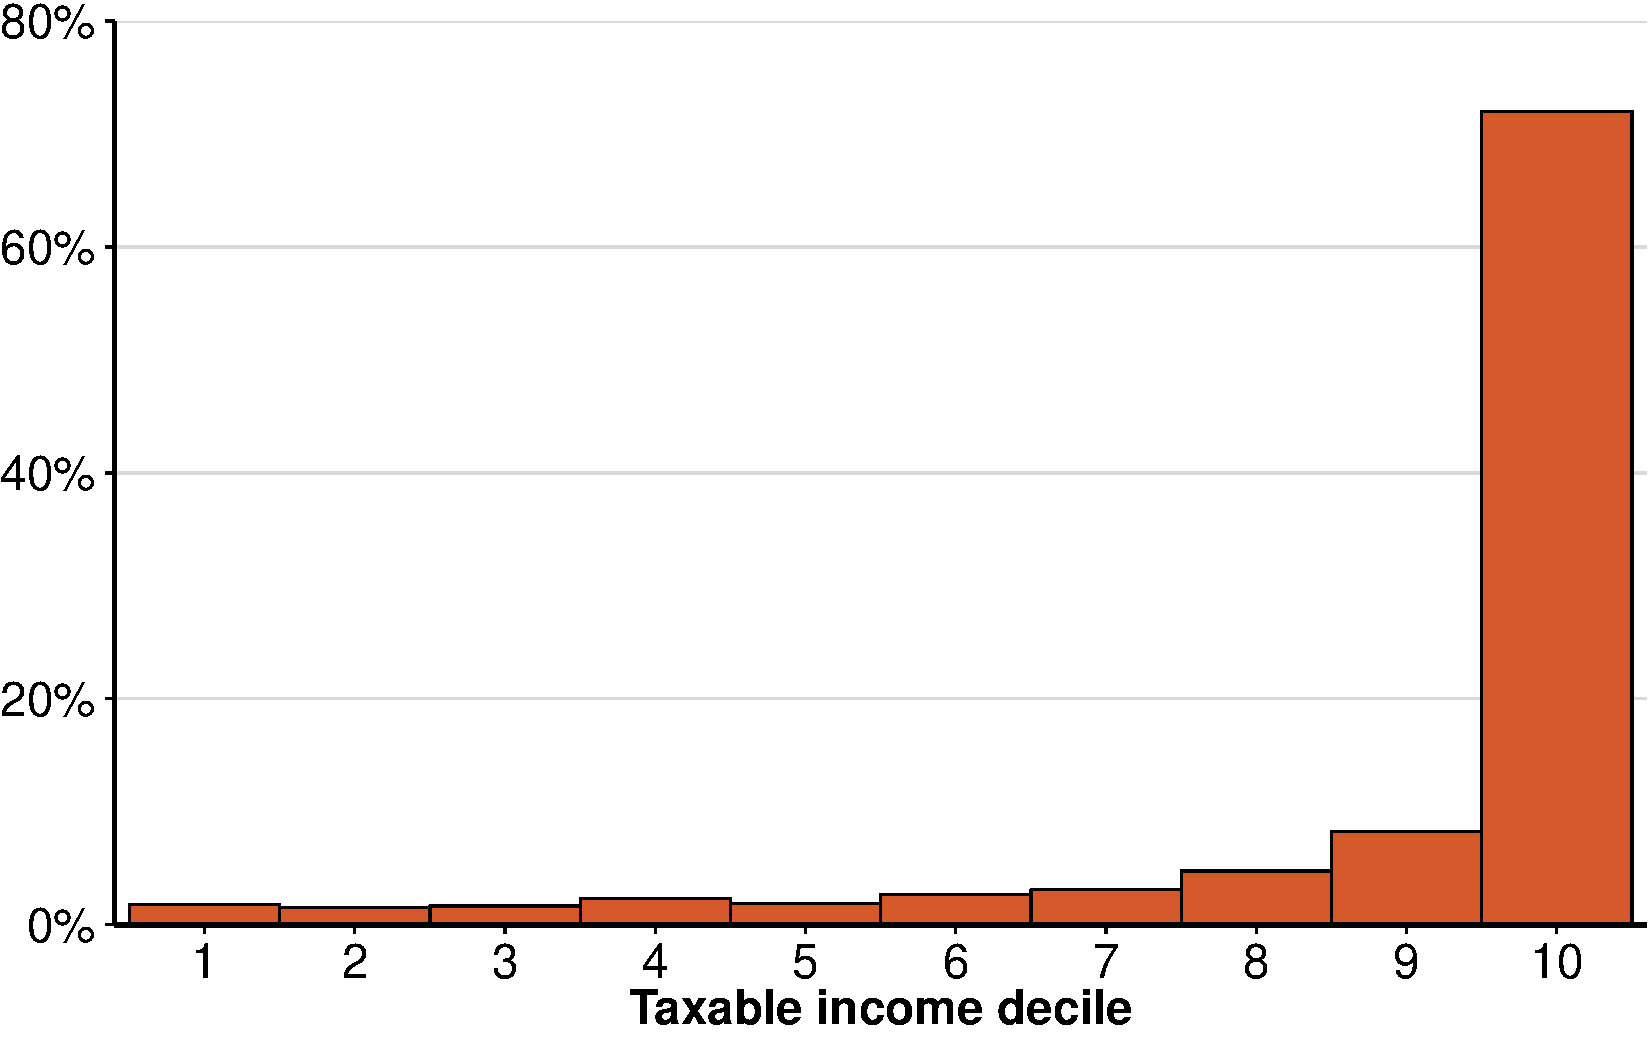
\includegraphics[width=\columnwidth]{CGT-NG-atlas//CG-by-decile-1}
\source{\gao\ \textcite{ATO2016SampleFile1314}}
\end{figure}

The proportion of gains accruing to those on high incomes may be somewhat skewed by the fact that capital gains are lumpy, so some lower income earners will have relatively high taxable incomes in the year they realise gains. But even if we look at the distribution of gains by taxable incomes \emph{before} capital gains, almost 40 per cent of gains are earned by the top 10 per cent of income earners. Another quarter is earned by those with very low taxable income\footnote{That is, less than \$10,000.}  – these tend to be two groups: over 50s who have waited until retirement to realise gains, but have much higher lifetime incomes (\Cref{sec:CG-receive-tax-advantages}); and some younger Australians, potentially partners of high income earners receiving distributions of capital income through structures such as trusts.\footnote{Most 30-45 year olds with no other taxable income receive very small capital gains. However, around 2.6\% of this group receive capital gains in excess of \$10,000 that make up more than 95\% of their total income. This small group pushes up the average capital gain for the bottom decile.} All of this only further demonstrates that capital gains accrue disproportionately to those who are already well off. 

Some inequality is acceptable if it is a consequence of some people working harder, or taking more risks, than others. But if the returns on savings concentrate resources even more than wage inequality, then the reinvestment of the returns on savings can lead to continued increases in the concentration of wealth – what Thomas Piketty described as an ‘endless inegalitarian spiral.’\footnote{\textcite{Piketty2013} highlights how returns on private capital have grown faster than the economy for much of history for a number of major economies. If this continues, wealth will become increasingly concentrated. \textcite[See also:][]{Leigh2013}.}

Critics of Piketty’s work, most notably Matthew Rognlie, argue that over the long-term, diminishing marginal returns should ultimately put a brake on the share of total income earnt by capital rather than labour.\footcite[][2]{Rognlie2014OnPiketty} However, Rognlie’s finding that higher house prices (and associated economic rents) have been the dominant driver of the growth in the capital share of national income\footcite[][3]{Rognlie2014OnPiketty} does not undermine Piketty’s thesis. Indeed, these findings suggest that so long as tight planning and zoning restrictions remain in place, those that can afford to save (and buy houses) are likely to keep capturing a growing share of national wealth.\footcite[See:][]{TheEconomist2015NIMBYs}  

Higher taxes on capital gains can break the cycle because they act as \emph{de facto} wealth taxes.\footnote{A sufficiently high tax on nominal gains amounts to a tax on wealth because it can eat into the real value of a person's assets over time: \textcite{Cowen2013}.}

Another cause for concern is that tax concessions for capital gains make Australia’s income tax system less progressive than its income tax regime suggests. While some may want a less progressive system, tax concessions are generally a poor way to achieve this, because they are inherently less transparent than changing the marginal rates of income tax. For value choices such as the progressivity of the tax system, the public debate is best served by making the distribution of the tax burden as transparent as possible.\FOOTNOTE{See \cpageref{paragraph:SUPER-progressivity-should-be-transparent} in \Cref{part:SUPER}.} %\footcite[][19]{DaleyCoatesWoodEtAl2015Super}

\section{Some discount may be justified but on balance the current treatment of capital gains is too generous}
When policy makers consider the taxation of capital gains, they must balance the competing considerations discussed above. 

All tax systems face this challenge. Most OECD countries offer some type of discount or concession for capital gains,\footnote{\textcite{Harding2013}. Although in some countries – including Denmark, Estonia, Iceland, Norway and Spain – property investments other than the family home are taxed as ordinary income.} although the hurdles to qualify for the most generous concessions can be high (\Cref{appendix:Intl-comparisons-of-CGT}).\footnote{For example, holding periods to receive maximum concession on investment property are ten years in Germany and Korea, 20 years in Slovenia, 30 years in France and 35 in Austria. \textcite[See:][]{Harding2013}. In New Zealand, where capital gains are notionally tax free, capital gains on property purchased with the intent to sell is taxed as ordinary income. \textcite[][See:]{InlandRevenueNewZealand2015MistakingPropertyDealingForPropertyInvestment}.} 

If the tax treatment of nominal capital gains simply aims for neutrality between immediate consumption and savings, then capital gains would be taxed a little more lightly than at present, under most scenarios for future returns.\footnote{Returns on property over the last 15 years may well have been usually high, driven by the fall in interest rates.} 

Yet this one-eyed treatment needs to be balanced against other considerations. Perhaps the most important is that people tend to save almost the same amount irrespective of the tax rate on savings.\footcite[][21]{Ingles2015} Higher taxes on capital gains would increase tax collections, help to repair the Commonwealth budget and provide room to reduce other taxes with higher economic costs. Higher taxes on capital gains would also reduce the tax bias toward capital gains and away from income producing assets, so that investment patterns would better reflect the economic fundamentals. They would also improve the integrity of the income tax system. 

Given that the tax is calculated on nominal (pre-inflation) capital gains, there remains some basis for continuing to offer a tax discount on gains. Reducing the discount from 50 per cent to zero -- in other words, taxing capital gains at the income tax rate – would substantially increase the real effective tax rate on savings. As we show in \Cref{chapter:options-for-reform}, a 25~per~cent discount for capital gains would provide a fairer balance.

\chapter{Negative gearing}
Negative gearing allows taxpayers to subtract the losses they make on investments from their taxable income, including wages. It has been widely used by property investors over the past 15 years. 

Negative gearing in Australia goes beyond generally accepted principles for offsetting losses against gains. It distorts investment decisions and increases the volatility of housing markets. Among its anti-social effects it reduces home ownership\footnote{Of course, owner-occupied housing also receives highly favourable tax treatment – it is exempt from capital gains tax and (net) imputed rents are not taxed. But as discussed on \cpageref{subsubsect:plausible-rational-for-encouraging-investment-in-owner-occupied-housing}, this reflects a deliberate policy choice to encourage people to purchase their own home. Overly generous tax breaks for investor housing undermine this objective.} and the availability of long-term rentals, but does not materially increase housing supply. It reduces tax collections, imposing pressures on the budget and creating the need for higher taxes or deficits. And it is regressive, benefiting those on high incomes much more than those on low incomes.

\section{Negative gearing provides a tax shelter against wages}\label{sec:negative-gearing-provides-a-widely-used-tax-shelter-on-wages}
Australian tax law allows investors to write off investment losses against their taxable income. For property investments, losses are defined as investment expenses in excess of rental income.\footnote{Of course a negatively geared investment is generally not making a real loss, but is accruing capital gain, which is not included in the definition of taxable income until it is realised: \textcites[][12--13]{ACOSS2015NGCGTHousing}[][11]{Carling2015}.} The greatest expense – about half the costs of property investors – is the nominal interest on borrowing to purchase the asset.\footnote{Half\DEVIATION{} of the costs of \emph{all} investors, including those who do not borrow, or who are positively geared.}

A property is \defi{negatively geared} if interest payments contribute to the rental losses.  

The interaction of negative gearing and tax concessions for capital gains provides some investors with a sizeable tax advantage. Taxes on capital gains are discounted by 50 per cent and only paid when the asset is sold. But negative gearing arrangements allow investors to deduct losses from wages and salary income that would otherwise be taxed at the full marginal rate. In some cases, negative gearing can allow a wage earner to pay less tax than if he\DEVIATION{} had not invested at all, despite also making profits on his investment (\Vref{box:NG-to-reduce-tax-on-wages}). 

Tax deductions from wage income may also generate a ‘psychic pay-off’ for some investors – the pleasure of an immediate reduction in tax. As an investment strategy, negative gearing only makes sense if the expected capital gains exceed the rental losses over the life of the investment. But for some investors, reducing taxes on their wages has become one of the primary goals. Investment advisors have warned against investors placing too much emphasis on tax breaks and not enough on the financial returns to the investment.\footnote{See for example: \textcite{Brown2012}.
There is some evidence from the US of taxpayers placing disproportionate weight on tax deductions for investments. For example, taxpayers are far more likely to contribute to a tax deductible retirement saving account if they owe money to the Internal Revenue Service in excess of taxes withheld, see: \textcite[][76]{HubbardSkinner1996}. The psychic pay-off is also reflected in the popularity of managed investment schemes for agriculture in Australia that allowed investors to claim the entirety of their investment as a deduction against their wages, although many of those schemes did not make attractive investment returns. See: \textcite{LaceyWaston2004}.}  

With the right investment strategy, an investor can use this asymmetry
in the tax treatment of gains and losses to pay less tax in total and
later despite receiving additional investment income (\Vref{box:NG-to-reduce-tax-on-wages}).

\begin{figure}[p]
\Caption{More people negatively gear property investments in their peak earning years}{Percentage of 2013-14 taxpayers within each age group}{fig:NG-PG-by-age}

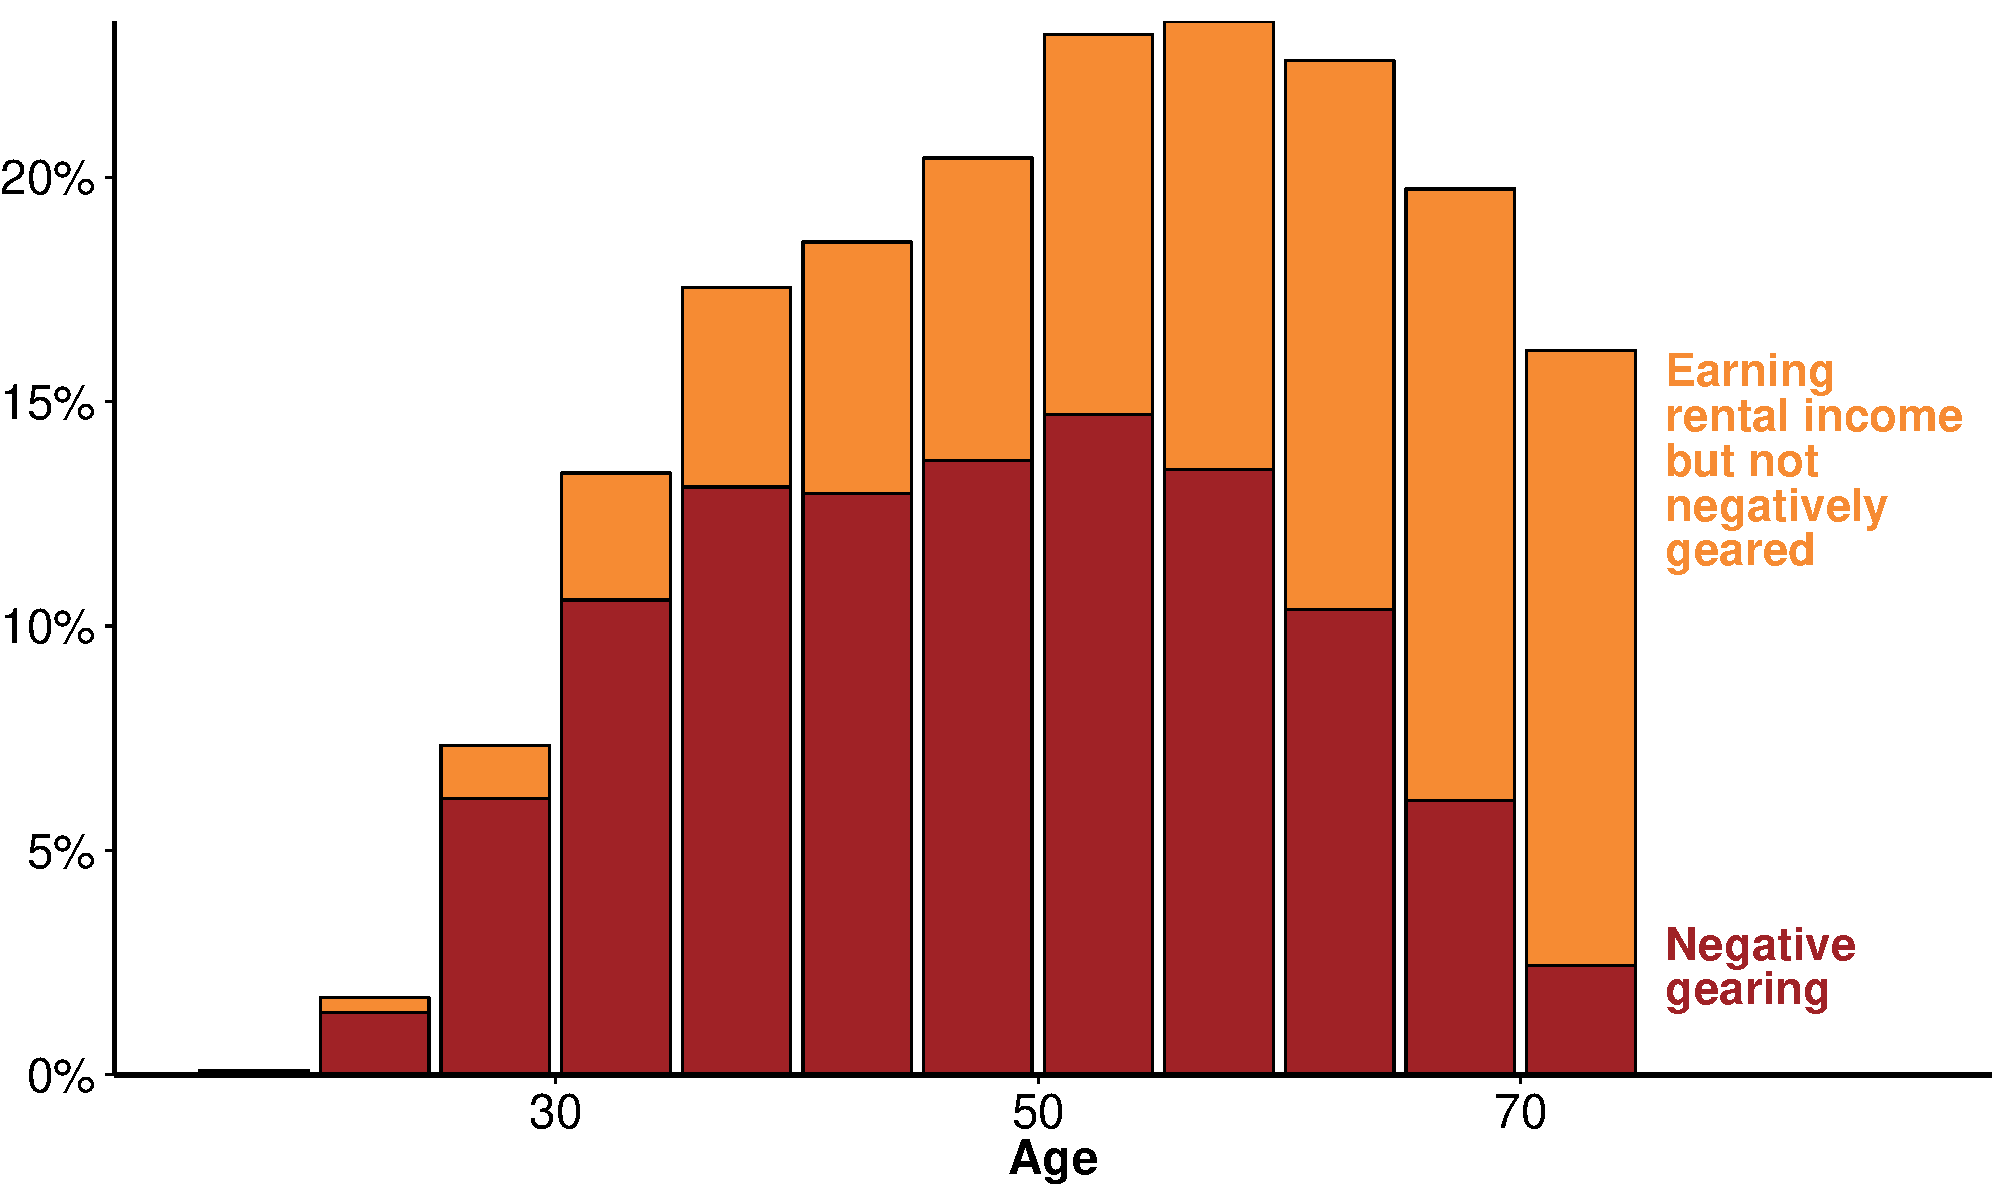
\includegraphics[width=1.22\columnwidth]{./CGT-NG-atlas/NG-PG-by-age-protrude.pdf}
\notes{Taxpayers over the age of 70 are not disaggregated in taxstats and have been presented as having ages 70-75.}
\source{\gao\ \textcite{ATO2016SampleFile1314}.}
\end{figure}

\begin{smallbox}{Using negative gearing to reduce taxes on wage income}{box:NG-to-reduce-tax-on-wages}
High income investors can maximise the tax shelter on their wage income
by borrowing to invest in assets that generate less in recurrent income
and more through capital gains.



Suppose Dan, a lawyer earning \$250,000 a year, 
borrows \$750,000 %
(interest only)
to purchase a \$750,000 investment property. Interest on the loan is 6~percent a
year and the property generates a rental return of 2.5~percent each
year. Most of the property's return is via capital appreciation of 5~percent each year.

In the first year, Dan makes a loss of \$26,000 
on the property and
reduces the tax he pays on his \$250,000 salary by 
\$13,000. His rental
losses decline over time as the property appreciates. After five years,
Dan has reduced taxes on his wage income by a total of 
\$70,000. If he
sells the property after five years he will realise a capital gain of
\$210,000 and pay tax on 
the gain of just under \$51,000.

Because of the asymmetry of tax treatment of gains and losses, Dan pays
\$8,700 less tax in total over five years than if he had not purchased
the house. So despite his profit of more than \$86,000 on the
investment, in effect he pays no tax on this profit, actually receiving a tax bonus.
\end{smallbox}

The attractiveness of using investment losses to reduce taxes on wage income is evident in the age profile of those negatively gearing property. Borrowing so much that the investment makes an annual loss is popular amongst those of working age, but far less prevalent amongst over 60s who are less likely to have labour income that can be offset by the tax loss. More than 70 per cent of those under 60 with investment properties make rental losses compared to less than 35 per cent of investors over 60 (\Vref{fig:NG-PG-by-age}).

Of course, not all investments are negatively geared. Some investors do not borrow at all, and others are ‘positively geared’ – the annual income on their property investment exceeds the annual costs of maintenance and interest. 
  
  Negative gearing is used much less for investments outside of housing. Investors in assets other than real estate, such as equities or unincorporated businesses, are less likely to borrow some of the funding, and usually do not borrow so much that these investments are negatively geared. 

Total lending to individuals for share investments is at most \$19~billion,\footnote{Individuals claimed \$1.1~billion in deductions for interest costs in 2013-14 (\textcite[][Table 12]{ATOTaxstats201314}), which excludes interest costs for rental properties. Assuming an average interest rate of 6~per~cent, the amount lent would be about \$19~billion. This is plausible: margin lending in 2013-14 was around \$11~billion (\textcite{RBA2015StatsMarginLending}), although not all of this would have been lent to individuals for share investing as some of this would have been lent to companies, and some would have been lent for managed funds. In addition to margin lending, individuals can borrow against housing to invest in shares.}  compared to individuals’ direct share holdings of about \$550~billion,  and compared to borrowings of \$548~billion from banks for housing investor lending.  


When individuals do borrow to invest in equities (known as a ‘margin loan’), the investments are seldom negatively geared. Equities investors are generally only negatively geared (that is, make losses after interest costs) when they use debt to finance at least 70 per cent of their investment.  The \emph{average} leverage of those who borrow to invest in shares is about 27 per cent.\footcite[][Table~D2]{RBA2015StatsMarginLending} Usually the maximum leverage permitted is about 75 per cent. And few margin-lending investors leverage more than 65 per cent of the value of their equity portfolio.\footnote{Most margin lending customers dislike margin calls, and so they tend to maintain a buffer of at least 10 per cent less than the maximum permitted leverage.}

Similarly, very few loans to invest in unincorporated businesses will be negatively geared. Banks are understandably reluctant to lend to businesses that do not have enough cash flow to cover interest payments. Total interest costs for unincorporated businesses were \$1.5~billion in 2013-14\footcite{ATOTaxstats201314} (much smaller than negative gearing against property), and much of this would have been incurred by profitable businesses. Total losses by unincorporate businesses were \$4~billion (see \cpageref{insec:number-taxpayers-claiming-business-losses} in \Cref{insec:number-taxpayers-claiming-business-losses}); many of these businesses would not have borrowed. 

\section{Negative gearing goes beyond generally accepted principles for offsetting losses against gains}\label{sec:NG-goes-beyond-accepted-principles-for-offsetting-losses}
The ability to deduct expenses incurred in generating assessable income is part of the normal operation of the Australian tax system, and applies to a wide range of investments and business activities. If losses were not deductible but gains were taxed, the asymmetry would make high-risk (high expected return) assets a less attractive investment. Deductibility of interest payments in theory also maintains tax neutrality for investors choosing between debt and equity financing.\footcite{FaneRichardson2004}   

But there is no theoretical basis for deducting losses on investments from entirely unrelated income such as wages. This is reflected in provisions that limit the deduction of business losses from wage and salary income.\footnote{If interest expenses were adjusted for inflation, and real gains were taxed annually as they accrue, this would present the strongest case for full deductibility of losses. But this is not the world we are in, and it is difficult to see a move to taxing accrued but unrealised gains given the issues this could cause for cashflow (\Cref{appendix:CGT-asset-lock-in}). Beyond the ‘in principle’ question of what income should be available for loss write-offs, quarantining losses from wage and salary income will reduce distortions by more closely aligning the timing of gains and losses.

A counter argument is that true symmetry in gains and losses would allow investors to claim back losses against previous tax paid on gains -- effectively lifetime smoothing of investment income. However, this is a largely theoretical concern with little impact on behaviour: few investors aim to make losses in perpetuity.} 

In some areas of tax and welfare policy, loss write-offs are already restricted. 
There are a number of limits on the deduction of business losses from wage and salary income.\footnote{If the business is a primary production business or a professional arts business, losses can only be deducted if other income (such as wages and salaries) is less than \$40,000 a year; for other businesses, losses can only be deducted if wage and salary income is less than \$250,000, and if the business has top-line income of at least \$20,000, made a profit in three of the previous four years, owns property worth at least \$500,000 used for a business activity, or uses other assets worth at least \$100,000: see \textcite{ATO2015OffsettingCurrentYearLosses}}
And income test calculations for welfare payments do not allow people to reduce their taxable income through investment losses. Income tests for Family Tax Benefit Part A and Part B, Child Care Benefit are all based on ‘adjusted taxable income’, which adds back any investment losses.\footcite{DHS2015AdjustedTaxableIncome} 
As a result, negative gearing is most restricted for those on lower incomes.

Very few advanced economies allow investment losses to be written off against wage income (\Cref{appendix:Intl-comparisons-tax-loss-deductibility}). 
The United States only allows loss write-offs against other forms of ‘passive’ income.\footnote{Passive income\label{footnote:passive-income} is more technically defined as income from rental properties or businesses in which the taxpayer does not materially participate. It is distinct from active income (wage, salary and income from business in which the person is actively involved) and portfolio income (income from interest, dividends etc). \textcite[See:][]{IRS2015}.} 
The UK only allows deductions against the same class of income, so for example, losses on investment property can only be used to reduce tax on income or capital gains from other investment properties. 
The Netherlands does not allow any deductibility of losses from investment housing (\Cref{appendix:Intl-comparisons-of-CGT}).\footnote{International regimes are summarised in \textcites[][43]{RBA2014SubmissionAffordableHousingInquiry}[][86]{ProductivityCommission2004FirstHomeOwnership}[][92--95]{ODonnell2005}.}

\subsection{Bias towards higher leverage}
\begin{figure}[!t]
\captionwithunits{Effective tax rates depend on amount of borrowing}{Real effective marginal tax rate}\label{fig:EMTR-by-gearing}

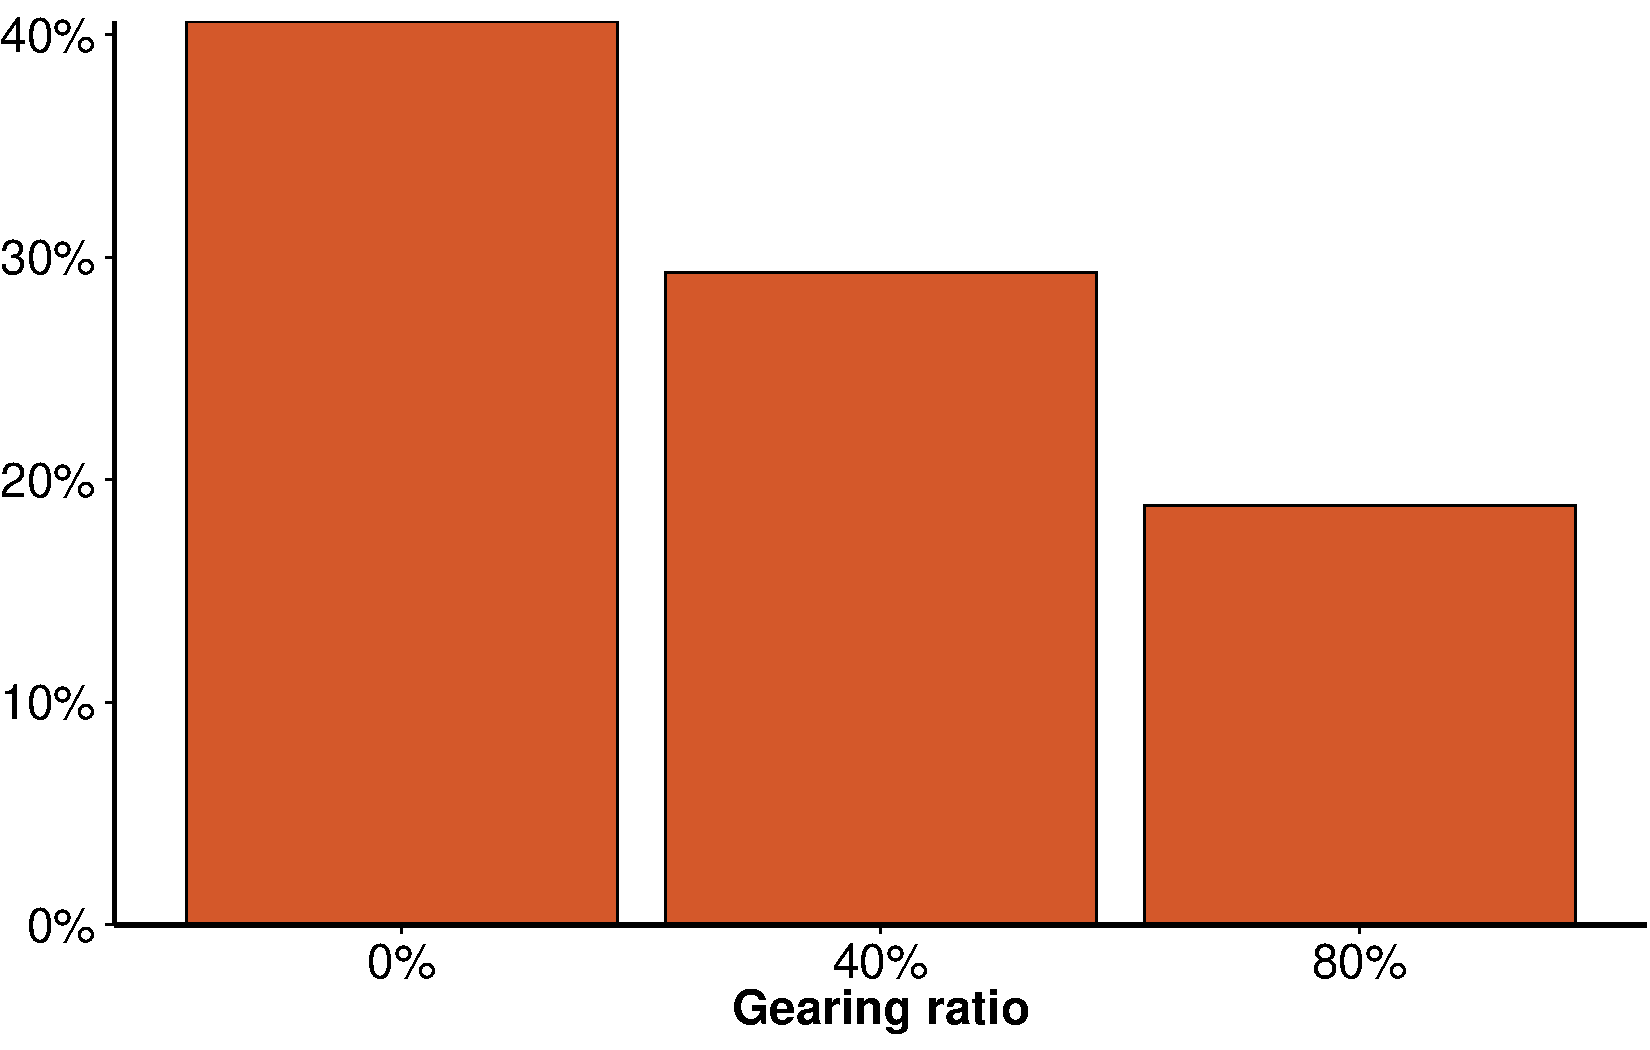
\includegraphics[width=\columnwidth]{CGT-NG-atlas//EMTR-by-gearing-1}
\notes{Assumes 
3~percent nominal rent income, 
5~percent capital gain per year, 
2.5~percent inflation,
5~percent interest rate on borrowing, 
50~percent CGT discount, 
and
47~percent marginal tax rate. 
The property is held for 
15 years and then sold.
}

\source{Grattan analysis}
\end{figure}

The asymmetry between the tax treatment of gains and losses makes debt financing of investment more attractive. Investors can write off their costs, including their nominal interest costs, in full each year. 
Gains, by contrast, are taxed concessionally and only when realised. 
A high-income taxpayer who invests in a rental property will enjoy substantially lower real effective marginal tax rates if she finances that property through borrowing instead of through existing savings. The higher she gears the property, the lower will be her effective marginal tax rate (\Vref{fig:EMTR-by-gearing}). 

The 2010 Henry Tax Review described this asymmetry between gains and losses as ‘among the greatest tax-induced biases to the savings choices of households’.\footcite[][69]{HenryTaxReview2010} This asymmetry weakens the argument that retaining the deductibility of losses is necessary to maintain tax neutrality.

While this bias towards higher leverage applies to all investments, in practice it encourages greater investment in property because bank lending rules allow greater leverage for property than for other assets such as shares (\Vref{sec:negative-gearing-provides-a-widely-used-tax-shelter-on-wages}).\footcite[][23]{RBA2015SubmissionHomeOwnershipInquiry}  


\subsection{Bias towards capital gains not annual returns}
The interaction of negative gearing and capital gains tax also biases the choice of investments. It means that for a given overall return, an investor will prefer an asset that pays less in the way of recurrent income and more in the way of capital gain.

As the RBA notes:\footcite[][42]{RBA2014SubmissionAffordableHousingInquiry}
\begin{quote}
\dots\ in most countries the earning of rental income is seen as the most important reason for investing in rental properties\dots. This seems to stand in contrast to the situation in Australia where properties are commonly marketed on the presumption that they do not earn positive taxable income for a considerable period.
\end{quote}

\textcite{seelig2009understanding} echoes the RBA view, finding that the majority of property investors saw capital gains as more important that rental income in motivating them to invest in property.\footnote{A clear majority considered capital gains as more important than rental income over a five and ten year time horizon. \textcite[][63]{seelig2009understanding}.}

\subsection{Investors have responded to these tax incentives}
\begin{figure}[!t]
\captionwithunits{The number of negatively geared investors has grown faster than number of property investors, and much more than their losses.}{1999-00 = 1.}\label{fig:number-NG-and-net-losses-time-series}
% 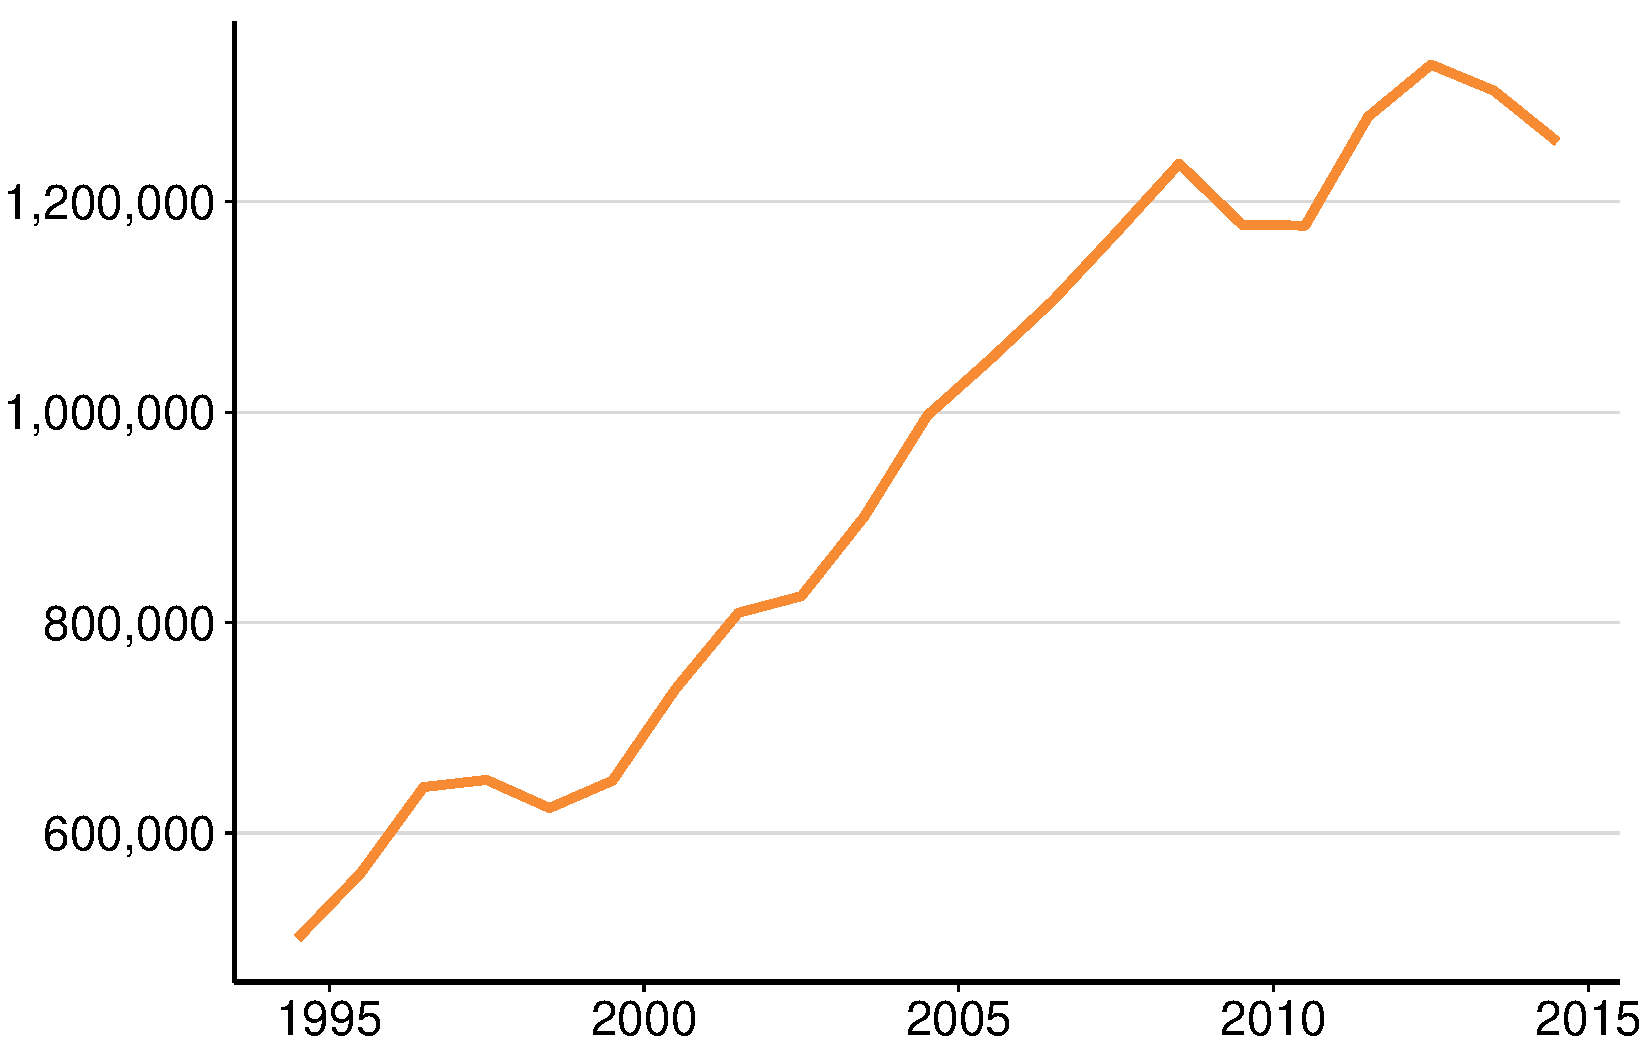
\includegraphics[width=\columnwidth]{CGT-NG-atlas//number-NG-time-series-1}
% \vspace*{4pt}
% \captionsetup{font = {small, color=theGrey}}
% \caption*{Average net rental loss, (2014-15 dollars)}\label{fig:number-NG-and-net-losses-time-series}
% 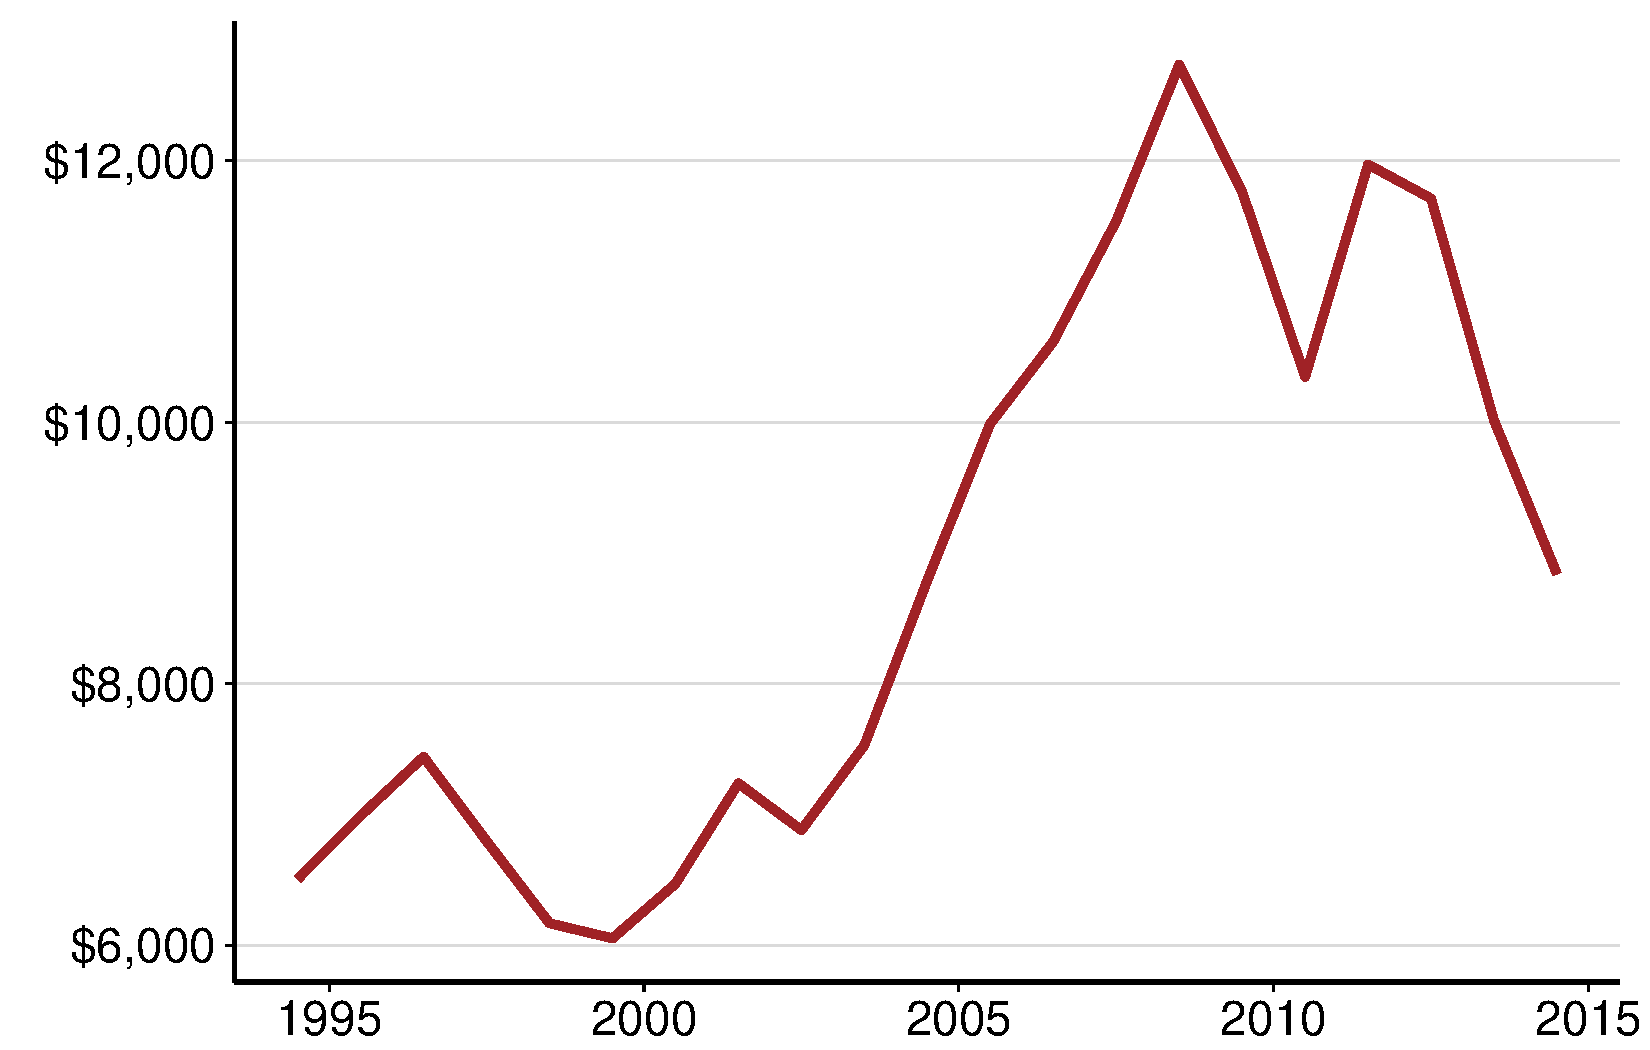
\includegraphics[width=\columnwidth]{CGT-NG-atlas//avg-net-losses-time-series-1}
\includegraphics[width=1.15\columnwidth]{CGT-NG-atlas/b5-palatino-atlas/CGT-number-NG-and-net-losses-time-series-1.pdf}
\source{\gao\ \textcite{ATO2016SampleFile1314}.}
\end{figure}


These biases are not just theoretical arguments. 
They are revealed in the changed behaviour of investors since capital gains tax changes increased the attractiveness of negative gearing from 1999.

Negatively geared residential property investments have grown rapidly over 20 years, particularly after 1999 when the capital gains discount changed from taxing all real gains to taxing half of nominal gains. 
Over 15 years the number of taxpayers making losses on residential property has almost doubled, as has the size of the average loss in real terms (\Vref{fig:number-NG-and-net-losses-time-series}).  






\textcite{seelig2009understanding} find that around half of investors would not have invested in property if negative gearing had not been available.\footcite[][63]{seelig2009understanding} 
Meanwhile there has been little change in the number of positively geared investors. Almost all the additional investors in property over the last 15 years were negatively geared (\Vref{fig:number-of-investors-by-gearing}).

\begin{figure}[!t]
\Caption{Almost all the growth in property investment since 1994 has been because of loss-making landlords}%
{Number of landlords, 1993-94 to 2013-14}{fig:number-of-investors-by-gearing}

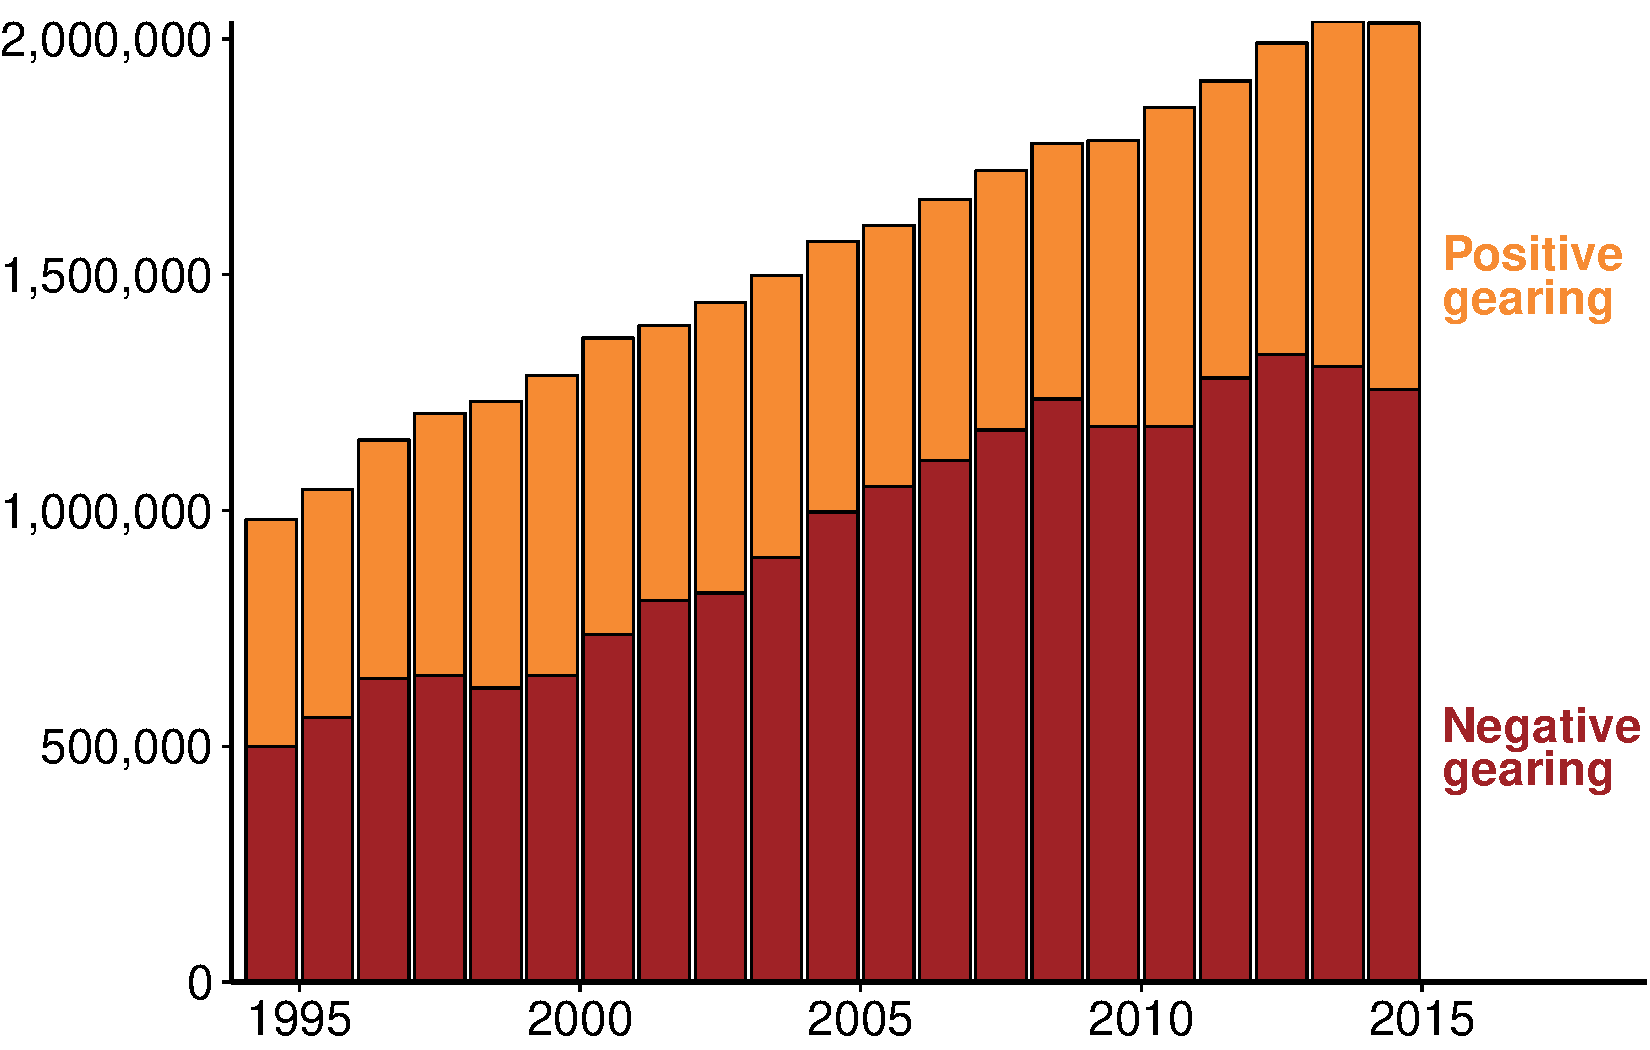
\includegraphics[width=\columnwidth]{CGT-NG-atlas//number-of-investors-by-gearing-1}
\source{\gao\ \textcite{ATO2016SampleFile1314}.}
\end{figure}

Another indication of the increase in negative gearing is that interest deductions as a proportion of rents rose from 46 to 84 per cent of gross rental payments in the 10 years to 2007-08. 
When interest rates subsequently fell, interest deductions as a proportion of gross rents fell to 55 per cent in 2013-14.\footcite[][65]{Treasury2015ReThink}


In their eagerness to pursue tax minimisation strategies, Australian landlords have moved from being collectively profitable, to accruing billions in net rental losses each year.
In 2013-14, 1.3~million landlords reported collective losses of \$11~billion. 
And total net rents have been consistently negative since the introduction of the CGT discount (\Vref{fig:Net-rent-time-series}).\footcites{Eslake2013}{ATOTaxstats201314}  
Losses are reducing only because interest rates have fallen.

\begin{figure}[htbp]
\Caption{Since the introduction of the capital gain tax discount, rental losses have been large, overwhelming profits}{Total real net rent (profit $-$ loss), individual taxpayers, (2014-15 dollars)}{fig:Net-rent-time-series}

\includegraphics[width=\columnwidth]{CGT-NG-atlas/b5-diana-atlas/CGT-Net-rent-time-bar-chart-1.pdf} % correct axis label
%\notes{Total net rent is the sum of net rental losses and profits across all landlords as marked on their tax returns.}

\source{\textcite{ATOTaxstats201314}}
\end{figure}

\subsection{Property churn}
The tax advantages encourage those with negatively geared properties to ‘churn’ investments. Over time, properties do not stay negatively geared. Rents tend to rise with increases in the value of wages, whereas the tax-deductible loan value cannot be increased.  So an investor who wants to stay negatively geared needs to sell, and then purchase another property with borrowings that are again a large proportion of the investment.

Consequently, negatively geared investors turn over their investments more often. 
\textcite[][28]{WoodOng2010} show that 40 per cent of all investors with rental properties retained their property at the end of a five-year period.  
Yet amongst investors who were negatively geared, only 20 per cent retained ownership. And a greater proportion of negatively geared landlords than other landlords purchased another property after selling.\footnote{13.1 per cent of negatively geared investors repurchase, compared to 11.2 per cent of positively geared investors. \textcite[][28]{WoodOng2010}.}  

\section{The distortions caused by negative gearing have undesirable social consequences}
Negative gearing has many undesirable consequences. It reduces rates of home ownership. 
It reduces the availability of long-term rentals. It increases the volatility of housing markets, increasing the risks to the Australian financial system. 

The favourable tax treatment reduces home ownership because it increases the after-tax returns to geared property investors but not homeowners. 
The increase in geared investing has made it harder for prospective owner-occupiers to afford to buy homes. 
Investors now account for more than half of new loans for housing, up from 29 per cent two decades ago.\footcite[][Table~8]{ABS2016a}  
This is one reason (though by no means the only one) why rates of home ownership are falling among younger age groups. 

The higher churn of properties encouraged by negative gearing also exacerbates a lack of secure long-term tenancies in Australia. 
Most of Australia’s housing stock is owned by landlords with only one or two properties, because progressive land taxes significantly reduce the returns from larger landholdings. (See \cpageref{paragraph:PROP-land-taxes-levied-on-progressive-scale} in \Cref{part:PROP}.) 
As many of these landlords are negatively geared, and want to turn over their properties in order to stay negatively geared, most Australian landlords are reluctant to agree to long-term tenancies. 
Their political interests have also led to Australian tenancy law providing much less security for tenants than in other countries.\footcite[][19--21]{KellyMaresHarrisonEtAl2013} 

The Reserve Bank, the Productivity Commission, the Henry Tax Review, and the Murray Financial System Inquiry have all argued that negative gearing exacerbates volatility in housing markets.\footcites[][88]{RBA2014FinancialSystemInquirySubmission}[][45]{RBA2014SubmissionAffordableHousingInquiry}[][75 \& 131]{ProductivityCommission2004FirstHomeOwnership}[][70 \& 418]{HenryTaxReview2010}[][278]{FinancialSystemsInquiry2015}
Negative gearing is most attractive as a tax minimisation strategy when asset prices are rising strongly. 
So in boom times it further increases investor demand for housing. 
The opposite is true when prices are stable or falling. 
Consequently, the greater leverage encouraged by negative gearing arrangements also reduces the stability of the Australian financial system.

There is little evidence that negative gearing has the socially desirable outcome of reducing rents, as \Cref{sec:Increases-property-taxes-will-not-change-rents} below discusses.

\section{Negative gearing mainly benefits those on higher incomes}\label{NG-benefits-those-on-higher-incomes}
Like most tax concessions on investment, tax benefits from negative gearing are regressive, benefiting those on high incomes much more than those on low incomes. A higher proportion of taxpayers on higher incomes negatively gear and the tax break is usually larger for individuals on higher marginal tax rates.\footcites{FinancialSystemsInquiry2015}{Grudnoff2015}

The fact that negative gearing is regressive is not in itself an argument for change, as mentioned earlier\DEVIATION{}. 
However, as that section argues, lower taxes on savings can concentrate wealth, and the inherent lack of transparency of tax concessions can undermine the overt choices that exist in income tax scales about the desired level of redistribution. 
So it is important to understand how the benefits of negative gearing are distributed. 
This analysis is also relevant to counter claims that negative gearing should be retained because it particularly assists those on middle incomes to build wealth. 

\begin{figure}
\Caption{More taxpayers on higher incomes negatively gear}{Distribution of taxable incomes by negative gearing status, 2013-14}{fig:tx-inc-distr-by-NG}
% dev omit emf due to alpha

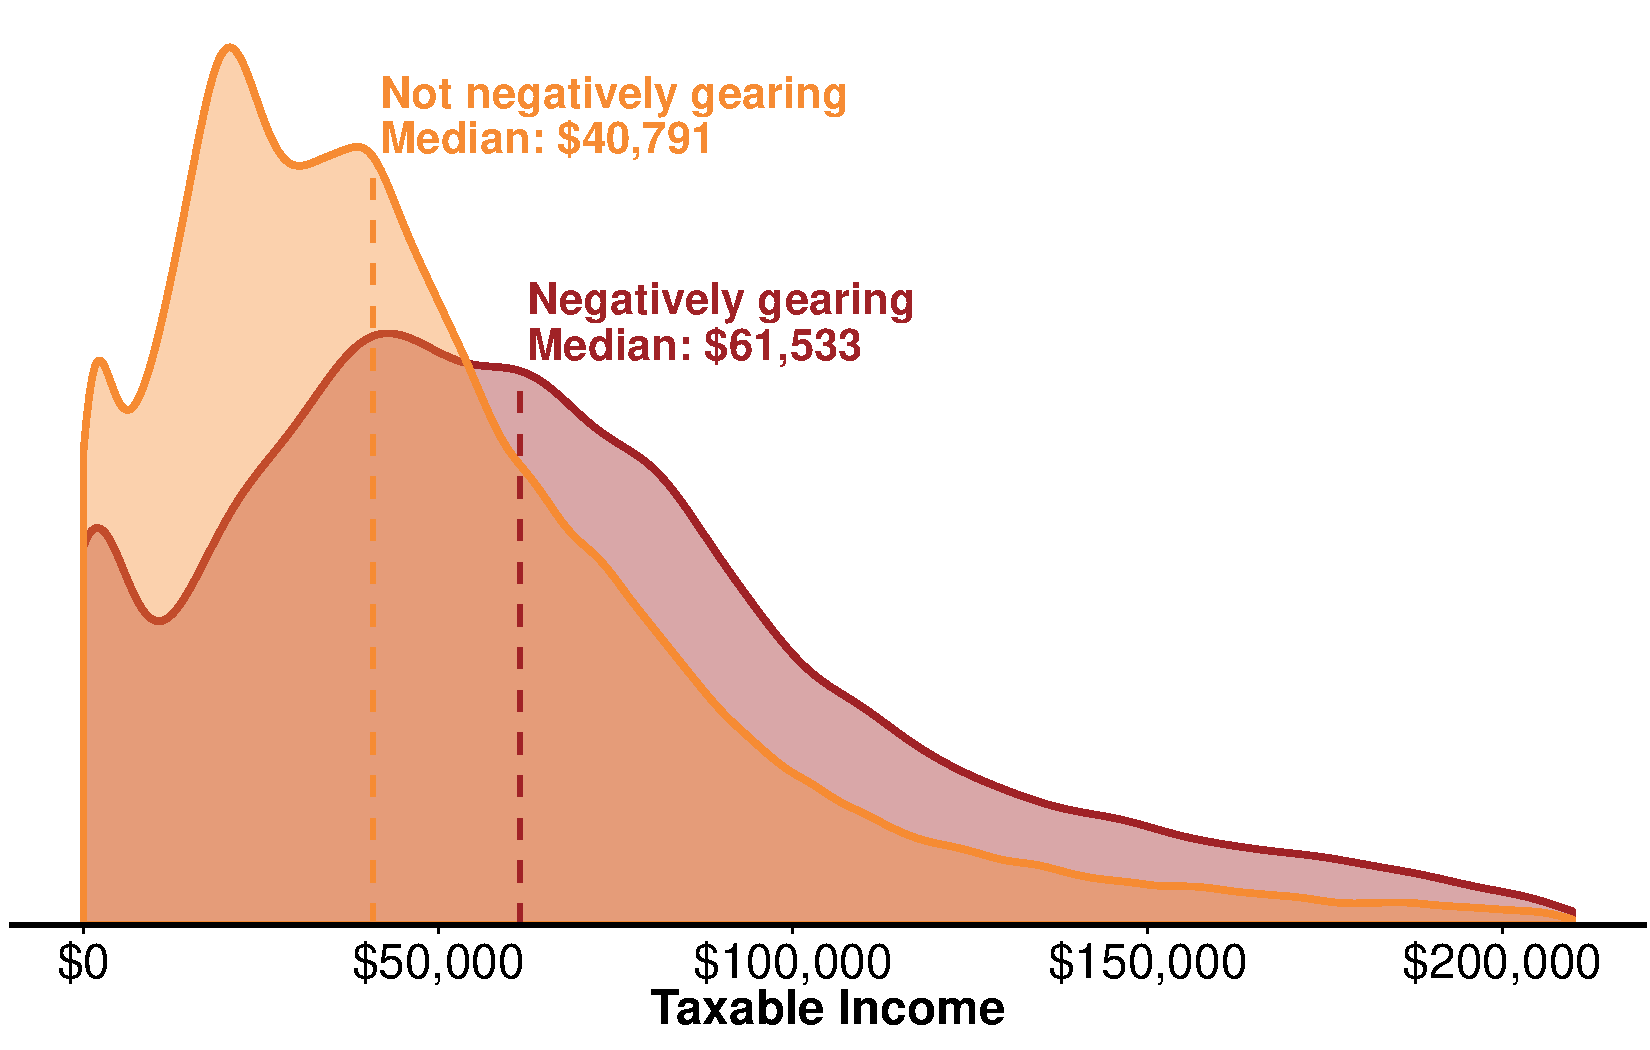
\includegraphics[width=\columnwidth]{CGT-NG-atlas//tx-inc-distr-by-NG-1}
\end{figure}

A lot of the public debate has centred on claims that most taxpayers negatively gearing have taxable incomes below \$80,000. This is not surprising given that only 20~per~cent of taxpayers have taxable incomes this high. 

People with higher incomes are more likely to negatively gear, as \Vref{fig:tx-inc-distr-by-NG} shows. The median taxable incomes for taxpayers who negatively gear is \$61,533 compared to \$40,791 for those who don’t negatively gear.\footnote{An \textcite{RBA2015SubmissionHomeOwnershipInquiry} analysis of \textcite{HILDA2015} also suggests that higher income earners are more likely to negatively gear property. It shows that the top 20 per cent of income earners are almost ten times more likely to have a debt-financed investment property than those in the bottom 20 per cent of earners.}

The tax benefits from negative gearing are even more skewed toward high-income earners. They borrow more on average, and with higher marginal tax rates, the deductions are worth more. 



Overall, the top ten per cent of income earners before rental deductions receive almost fifty per cent of the tax benefits of negative gearing. 
The skew does not look quite so bad if taxpayers are grouped by their taxable incomes, as shown in the left hand side of \Vref{fig:Benefit-NG-before-after-deductions}. But comparisons based on taxable incomes understate the earnings of those negatively gearing. 
Taxable incomes are assessed after rental losses. 
In other words, people who are negatively gearing have lower taxable incomes because they are negatively gearing. 
The taxable income distribution before rental deductions, shown on the right hand side of \Cref{fig:Benefit-NG-before-after-deductions}, shows that those on higher incomes receive the lion’s share of the tax benefits from negative gearing. 

The skew of negative gearing benefits is also obvious when looking at occupations. Despite claims from the Property Council that lower paid workers such as nurses, teachers and clerical staff are the ‘primary beneficiaries’ of negative gearing,\footcite{PropertyCouncilAustralia2015WhoReallyUsesNG} analysis of Australian Tax Office (ATO) data shows that a higher proportion of workers in high-wage occupations negatively gear and receive larger average tax benefits when they do so (\Vref{fig:NG-by-occup}).
\begin{figure}
\Caption{Negative gearing mostly benefits those on high incomes, and the difference is especially stark when incomes are measured before subtracting rental interest deductions}{Percentage of each decile's share of the benefit in reduced income tax due to negative gearing (2012-13)}{fig:Benefit-NG-before-after-deductions}
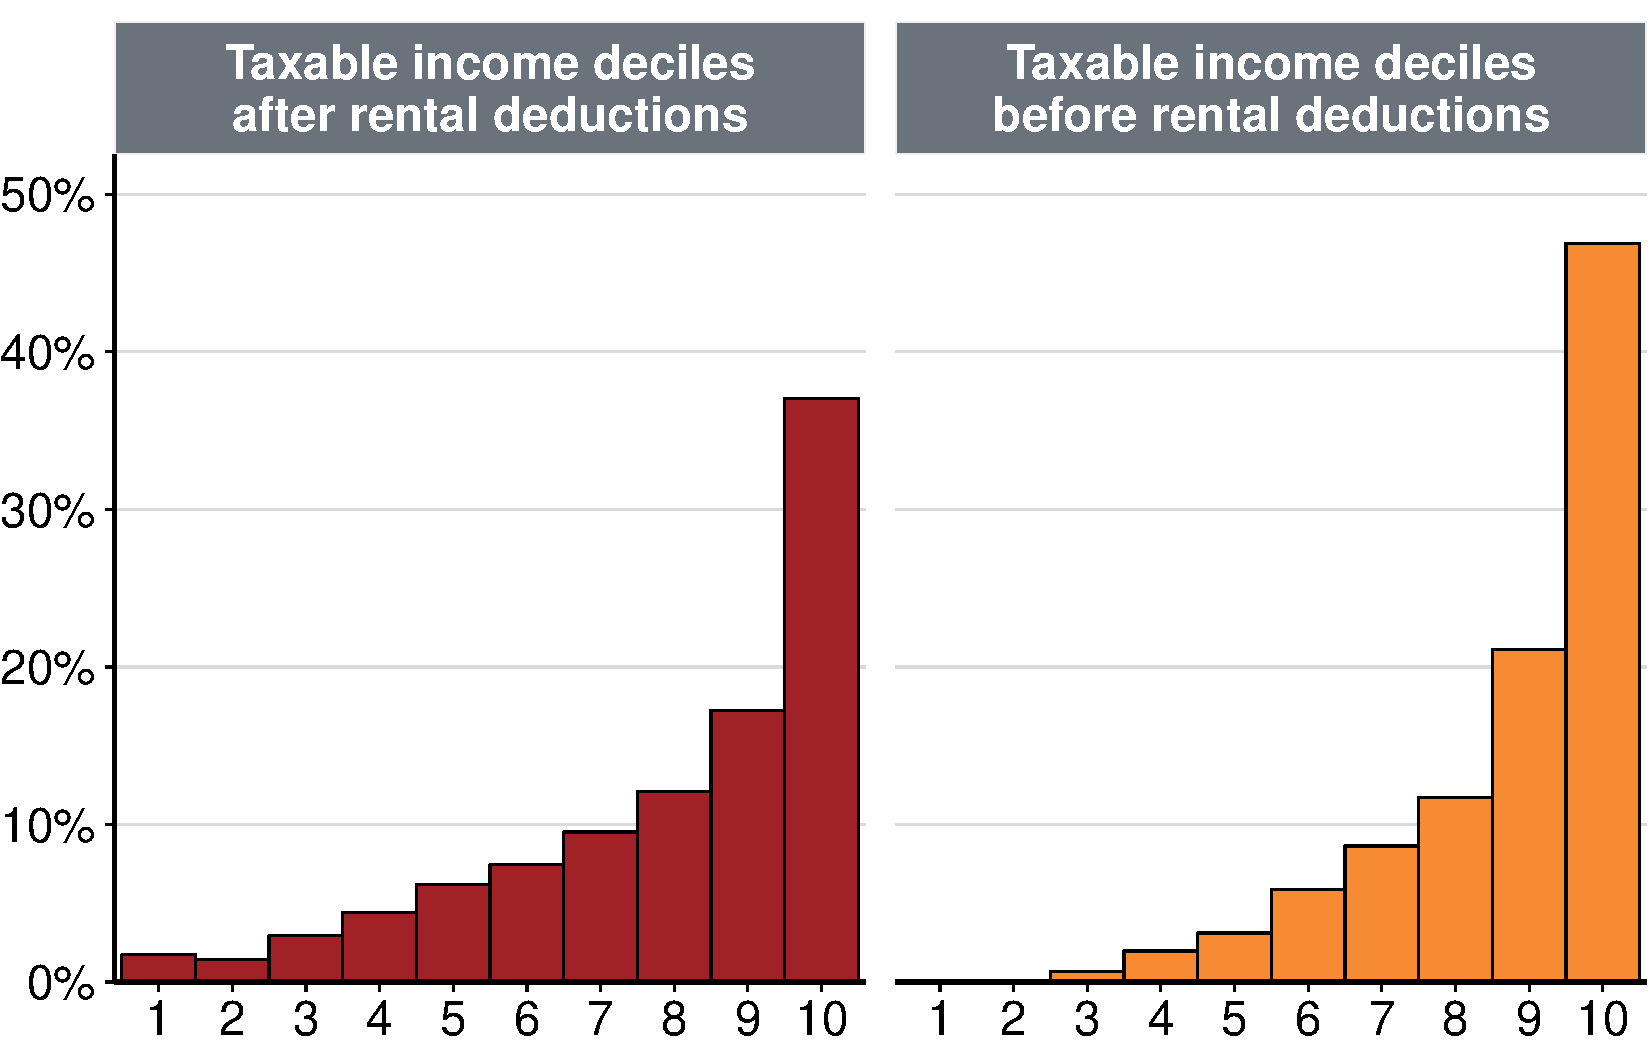
\includegraphics[width=\columnwidth]{CGT-NG-atlas//Benefit-NG-before-after-deductions-1}
\notes{Taxable income before rental deductions means Taxable Income minus rental loss. 
Income tax includes medicare levy, \textsc{lito}, and the temporary budget repair levy but not other tax benefits (\emph{e.g.}~the seniors and pensioners tax offset (\textsc{sapto}))}

\source{\gao\ \textcite{ATO2016SampleFile1314}.}
\end{figure}

\begin{figure}
\captionsetup{justification=raggedright, singlelinecheck=false}
\caption{Those in high-income occupations are more likely to negatively gear, and receive more of the tax benefits}\label{fig:NG-by-occup}
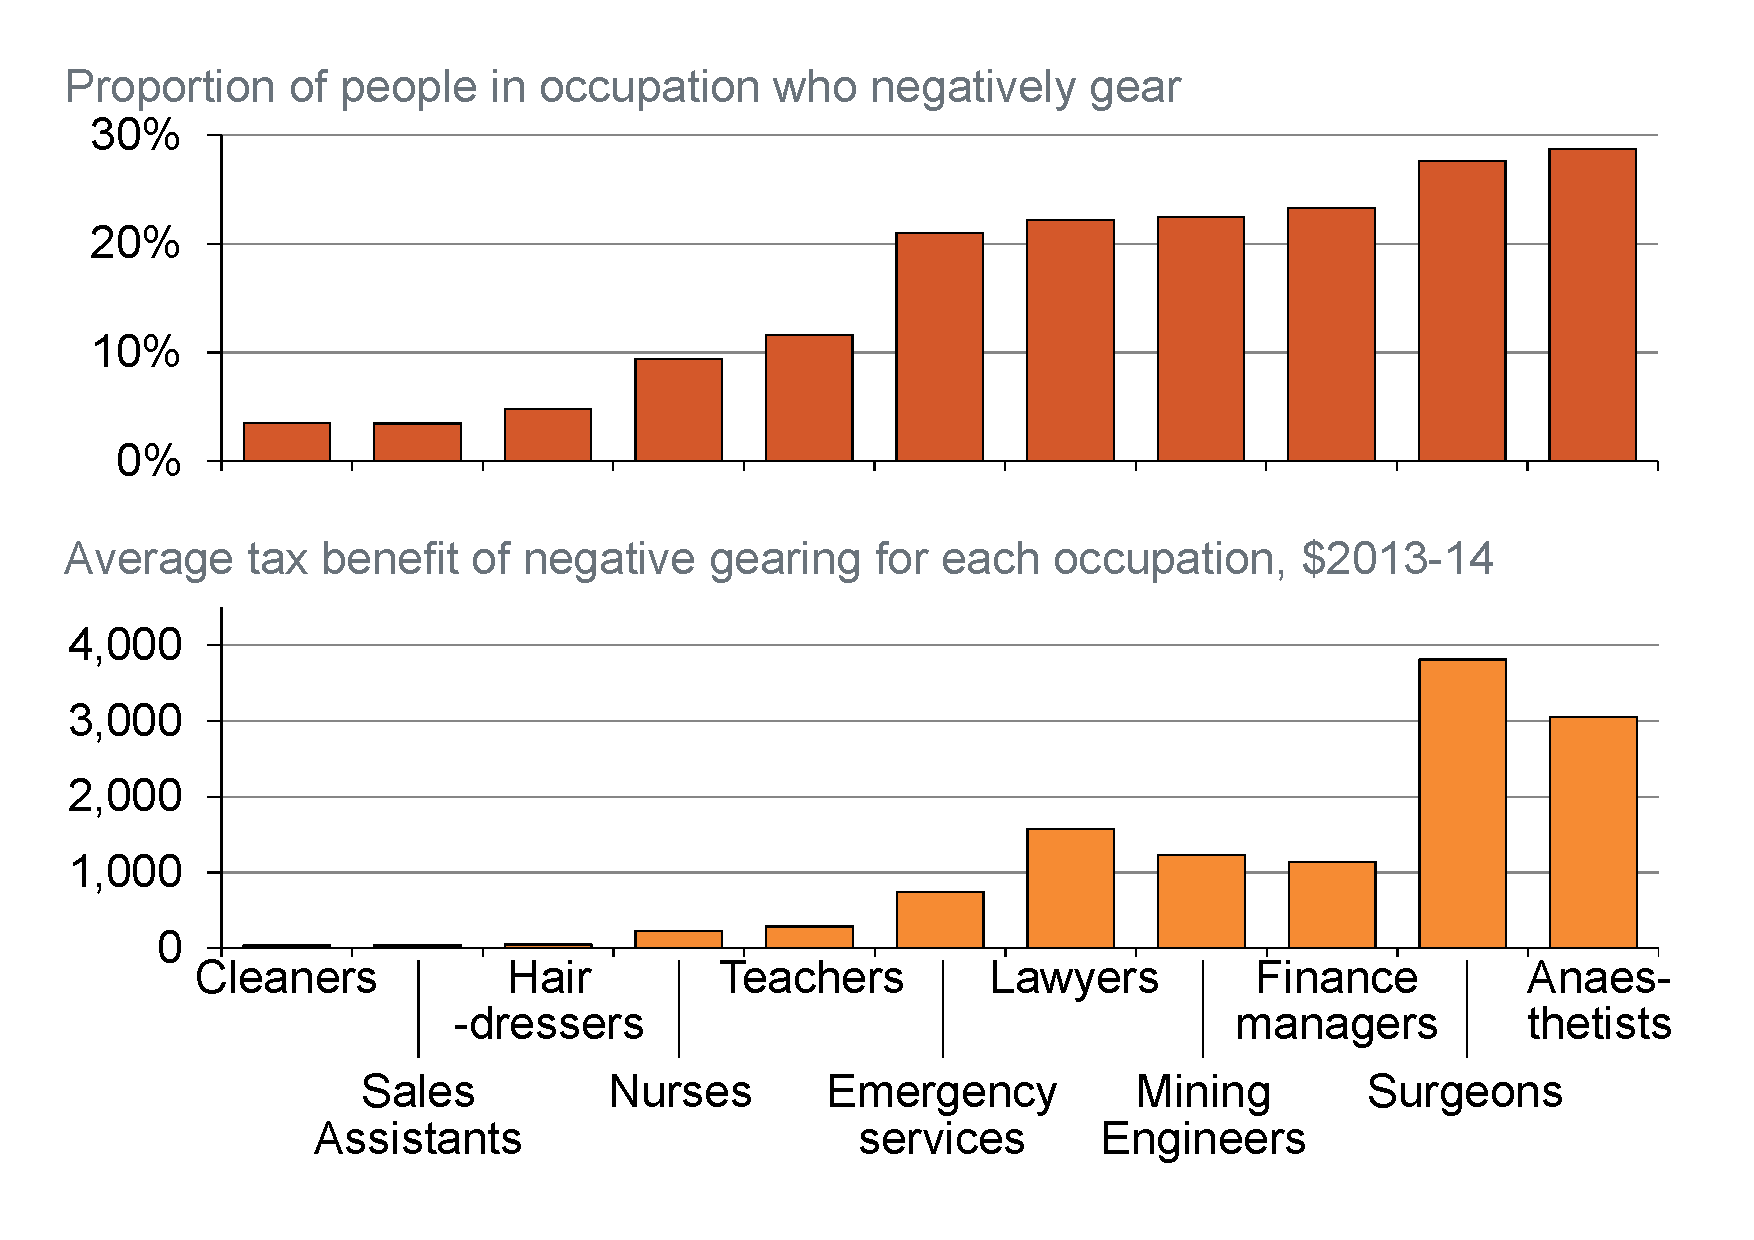
\includegraphics[width=\columnwidth]{CGT-NG-atlas/Occupation-pptx.pdf}
\notes{Average tax benefits are calculated by deducting average rental losses at the tax rate associated with average taxable income for that occupation. }

\source{\textcite{ATOTaxstats201314}.}
\end{figure}

%\flushcolsend
\chapter{Impact of changing negative gearing and the CGT discount}\label{chapter:Impacts}
Reduction in the CGT discount and changes to negative gearing will affect investor demand, rents and property prices. Yet the impacts will be much smaller than some commentators suggest. 

This chapter outlines how the housing market would be affected by the changes we propose to the tax treatment of investments – reducing the capital gains tax discount to 25 per cent and quarantining investment losses so they cannot be written off against wage income. 
These proposals are explained in more detail in Chapter 5. 

Our best estimate is that the changes we recommend might lead to property prices up to 2 per cent lower than otherwise. There will be little impact on rents, or on the rate of new development, even in the long-term.


\section{Tax changes will somewhat reduce investor demand}
Reducing the capital gains tax discount and limiting scope for loss write-offs by changing negative gearing arrangements will somewhat increase effective tax rates for property investors, thereby reducing their demand for property. 
However, the changes in after-tax returns are unlikely to have radical effects on demand for investment property.

Some investors will switch to other investment opportunities that offer higher post-tax returns. Others might choose to spend more and invest less. But some will also continue to invest in the housing market, and either borrow less, or simply accept a lower return on investment. Others may put more into their principal residence – choosing a larger or better-located dwelling – rather than investing in a second property.

The extent to which investors will vacate the property market will ultimately depend on how much post-tax returns fall, and how sensitive investor demand for property is to changes in returns (what economists would call the ‘elasticity of demand’).

Our analysis shows that the effective tax increases from our proposed changes to negative gearing and capital gains tax are relatively modest (\Cref{sec:Summarizing-impact-proposed-NG-and-CGT}). 

Switching into other asset classes will be limited. Other investments that generate capital gains, such as shares, will also be taxed more under proposed changes to CGT and negative gearing (\Cref{chapter:options-for-reform}). Other investments that will be relatively more attractive after the change – for example, bank deposits and superannuation – have very different risks, returns and liquidity. As a result many investors may choose not to switch. 

Ultimately people who invest in property take into account a host of factors, including rental returns, risk perception, familiarity with the asset class, and ability to obtain bank finance. Modest changes in tax treatment will not affect their decisions much. (\Cref{sec:What-is-the-right-tax-rate-on-capital-gains})

Indeed, countries with less generous tax treatment for investment properties – US, Canada, Germany and France, for example – still have plenty of investor activity in housing.\footcite{ABS2010MeasuresOfAustraliasProgress}



\section{House price impacts will be relatively modest}
Economic theory suggests that higher property taxes and reduced investor demand will lead to some combination of higher rents and lower property prices. But in urban housing markets with tight constraints on supply almost all the impact will be on residential property prices rather than on rents.

If higher taxes are fully passed through into house prices, they are unlikely to fall by more than about 2~per~cent. This reflects the magnitude of the proposed tax changes relative to property prices and the fact that about two thirds of buyers – owner-occupiers – will be not be directly affected by the tax changes (\Vref{box:ImpactOfPrice}).\footnote{This estimate is similar to that made by \textcite[][154]{AbelsonJoyeux2007}. They suggest the tax subsidy associated with the asymmetric treatment of gains and losses by housing investors (i.e., the interaction of negative gearing and the capital gains tax discount) is about 1.6~per~cent of annual housing value (p.154). This paper also models the effect of a 10 per cent increase in tax on rental incomes – larger than effective changes from our policy (\Vref{box:ImpactOfPrice}) – it estimates a 3 per cent decrease in house prices.}

Tax changes that might only drag down house prices by 1 or 2 per cent should be put in perspective. House prices have grown annually by an average of 7.3 per cent since 1999.\footcites{ABS2015ResidentialPropertyIndex}{Yates2011}
Such a tax change corresponds to a few months’ growth lost (or a few months to defer a sale).

Consequently tax policy is a minor risk to house price growth.  Interest rates, terms of trade, changing expectations about the economy, and zoning and planning policies are much more important. As CBA Chief Executive Ian Narev recently noted:

\begin{quote} 
\textit{I can tell you this, having a \$400 billion home loan book: your assumptions on unemployment and what's happening in global interest rates will dwarf whatever assumptions you've got on the modelling about the impact of negative gearing by a factor of---I can't tell you the number. It's a big number.}
\end{quote}

Such price falls would not lead to widespread negative equity – investors owing their lender more than the value of the property. Even in locations where investment property is concentrated, tax changes would not affect prices by more than 4 per cent (\Cref{tbl:Impact-house-prices}). And less than 10 per cent of new property loans go to investors with loan to value ratios (LVRs) over 90 per cent.\footnote{For the December quarter of 2015, 9.7 per cent of new residential property loans had a loan to value ratio of greater than 90 per cent, and almost a quarter have a loan to value ratio above 80 per cent. See: \textcite{APRA2016PropertyExposures}.}

What’s more, tighter macro-prudential controls on bank lending are expected to reduce the proportion of high LVR loans in future.\footnote{\textcite{APRA2014a}. See \textcite{Schlesinger2015} for a discussion of the impact on bank lending practices and LVRs.}  
  And few loans stay at such high leverage for long.  For the small proportion of investors that remain highly leveraged, higher interest rates pose a far greater risk than changes to the tax treatment of rental losses.\footnote{The leverage on many existing loans has fallen because property prices rose, and a material proportion of investors chose to get ahead on their mortgage repayment schedule. See: \textcite{RBA2015StatsMarginLending}.} 

The Australian Government should not shy away from a sound policy because it generates modest house price corrections. 
This is especially true given that affordable housing is an avowed policy goal. It is difficult for governments to address housing affordability for new buyers while continuing to offer generous tax breaks to investors that bid up house prices. 


\section{Increases in property taxes will not change rents much}\label{sec:Increases-property-taxes-will-not-change-rents}
The potential effects of tax changes on rents are perhaps the most contentious. Concerns persist that limiting negative gearing or reducing the capital gains tax discount will reduce the supply of rental properties and push up rents. 

To some extent these claims are based on experiences from the 1980s, particularly in Sydney. 
In 1985, the Hawke Government restricted negative gearing so that rental losses could not be used to reduce tax payable on other income streams.\footnote{\textcite[][20]{McKellInstitute2015SwitchingGears}  The measures only applied to real estate purchased after 17 July 1985.}
Rents rose rapidly in Perth and somewhat in Sydney. 
Two years later, the policy was abolished out of concern for increasing rental prices. 

\begin{figure}
\Caption{Rents did not rise when negative gearing was removed in Melbourne, Adelaide or Brisbane}{Average rent prices (real compared with overall CPI), 1982 = 1.
Grey band indicates the dates when negative gearing was not permitted}{fig:Capital_city_rents}
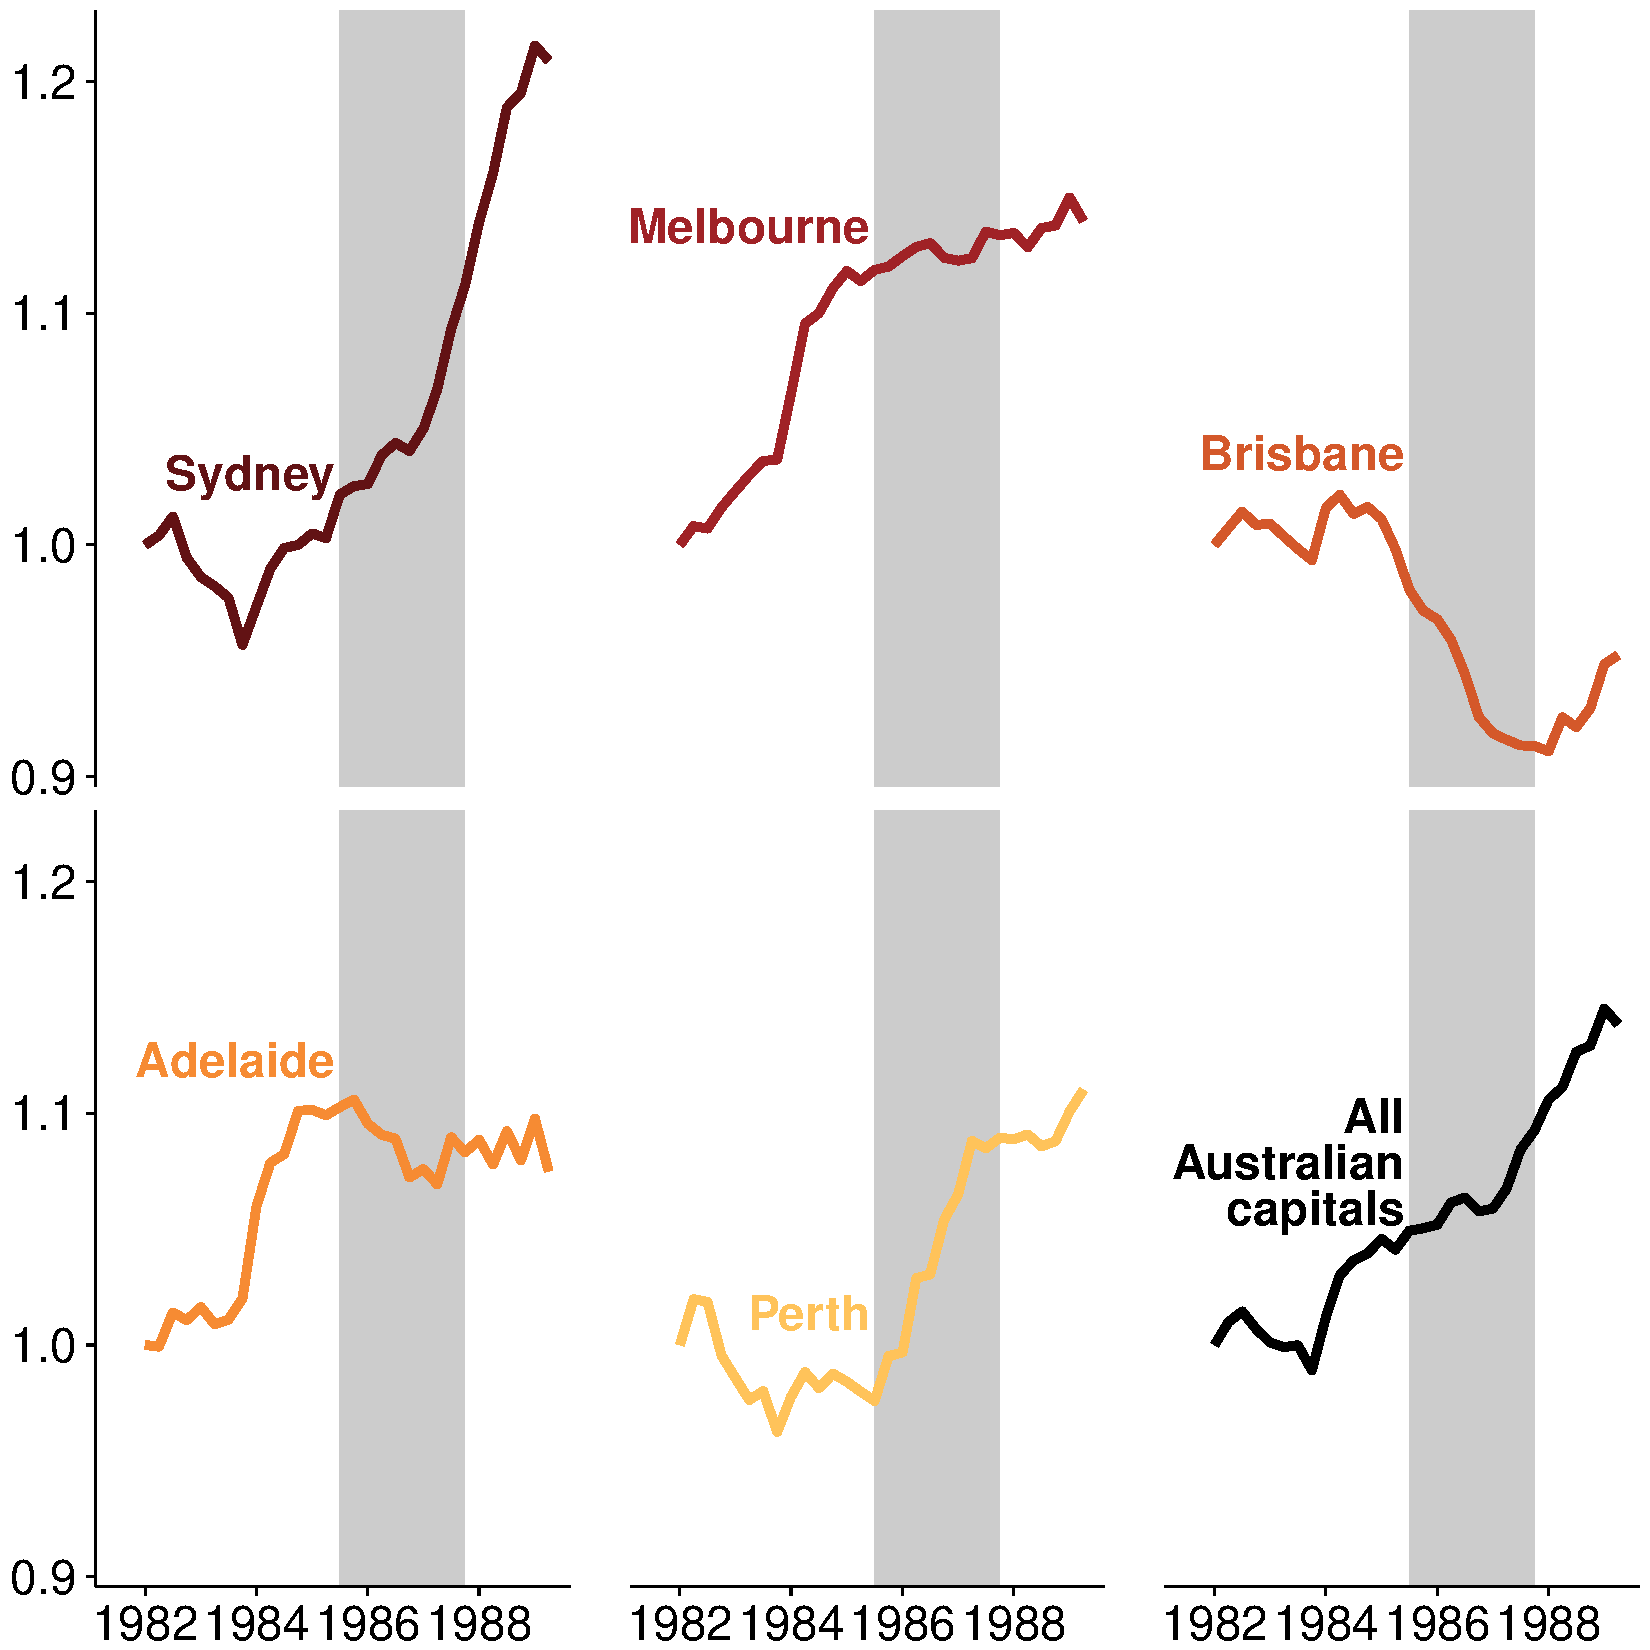
\includegraphics[width=\columnwidth]{CGT-NG-atlas/b5-palatino-atlas/Capital_city_rents_direct_abs-1}
\source{\textcite{ABSVariousyearsCPI}}
\end{figure}

History might have taught a different lesson if fewer of Australia’s Prime Ministers and Treasurers came from Sydney. Although the tax changes were nation-wide, inflation-adjusted rents were stable in Melbourne and actually fell in Adelaide and Brisbane (\Vref{fig:Capital_city_rents}). In Sydney and Perth, rent rises were in fact driven not by tax changes but by population growth and insufficient residential construction – due to high borrowing rates and competition from the stock market for funds.\footcites[][186]{BadcockBrowett1991}[][47--48]{DaleyMcGannonSavageEtAl2013BalancingBudgets}

Studies of overseas experience also suggest that changes to the taxation of property investment have limited impact on rents, even over the medium term. These studies find that rent increases in response to tax changes are modest\footcite{DiPasqualeWheaton1992}  and very slow to take effect, with most impacts not seen for more than a decade.\footnote{\textcite{BlackleyFollain1996}\label{footnote:BlackleyFollain} show that only a fraction of higher investment costs are ultimately reflected in higher rents, and even then, there is very limited discernible effect for a decade after any tax changes. Even \textcite{Poterba1992} who argues that changes in the tax treatment of investor housing should be reflected in higher rents, failed to find any short term impact. Real rents grew more slowly in the United States after 1986 when negative gearing was restricted and depreciation allowances were made less generous.}\label{endnote:BlackleyFollain}

Beyond these historical lessons, economic theory and empirical research show that limiting negative gearing or increasing taxes on capital gains does not change rents much. In urban areas where land supply is restricted and rents are determined by location-specific factors such as access to transportation and amenities, tax changes primarily affect property (land) prices rather than rents.%
\footnote{\textcite{CapozzaGreenHendershott} \textcite{StapledonRoberts2016} highlight that in the long run the relative shares of the cost of development versus land value (locational premium) determine the relative impact on rents and prices. Closer to the cities where land value is a larger component of property value, changes in tax will mainly change prices. For apartments and properties on the outer edges where structure is a larger share of the value, the effect on rent may be somewhat larger (and the effect on land prices smaller). However, given the size of the tax concession in the context of the overall market (\Cref{box:ImpactOfPrice}), any impacts on rents for these properties are still likely to be modest.} 

In the short term, tax changes reduce the post-tax investment returns for negatively geared property investors. There will be a one-off decrease in house prices as investors reduce their willingness to pay for property. But because rental yields are calculated as a proportion of property prices, they will rise as house prices fall. This rise will at least partially restore the attractiveness of property investment relative to other investments. 

Existing negatively geared investors will have larger post-tax losses to service. They may want to increase rents to maintain their returns. But rents are determined by dynamics of demand and supply, not by the returns that owners are seeking. Rents do not increase just to ensure that buyers of assets get their money back.\footnote{This assumption is the basis for claims in some papers that tax changes for investment housing will have much larger impacts on rents than we estimate. For example, \textcite{AbelsonJoyeux2007} estimate a 10 per cent increase in tax on rental incomes would lead to a 7 per cent increase in rents and a 3 per cent decrease in property values (p.160). However, they assume that markets return quickly to an equilibrium at which returns equal the returns on other assets in the same risk group. As the empirical evidence summarised at \cref{footnote:BlackleyFollain} shows, in reality any impact on rents is likely to be smaller and slower to take effect. } 

Existing negatively geared investors compete to supply rental properties against other property investors with no imperative to increase rents. The tax changes will not affect rental incomes for the one-third of landlords making positive rental profits. And new investors would purchase properties at lower prices that factor in the less generous tax treatment of rental losses. Tenants can beat rent rises by threatening to move to properties owned by these other investors. 

Some negatively geared investors may sell their properties to owner-occupiers if tax concessions are less generous. But in the short term this has no impact on rents.  Every time an investor sells a property to a renter, there is one less rental property, and one less renter. There is no change to the balance between supply and demand of rental properties. Others may sell to another investor, but one that doesn’t rely on negative gearing. Again this doesn’t reduce the number of rental properties. 

\section{Impact on new development is also likely to be small}\label{sec:Impact-new-development}
Over the longer term, lower after-tax returns to investors could slow new housing construction and put upward pressure on rents.\footcites{Poterba1984}{AlmFollain1994} But the tax changes proposed are unlikely to substantially alter the incentives for new development as some have claimed.\footnote{\textcite{BISShrapnel2016} cited in \textcite{Daley2016onBIS}.} One-off price impacts of less than two per cent (\Cref{box:ImpactOfPrice}) are unlikely to substantially slow new construction.

The main constraint on new housing is land release and zoning restrictions – especially in established suburbs with good access to jobs and transport.\footcites{KellyHarrisonHunterEtAl2013}[][84--90]{KellyDonegan2015} In this environment, any changes to the price of housing are likely to be incorporated into the price of land rather than the amount that people are prepared to pay for developments. 

In any case, general tax breaks such as negative gearing are an inefficient way of supporting the rental market.\footcite{HenryTaxReview2010} Between 8 and 14 per cent of all investment property lending is for new dwellings.\footnote{The most recent ABS lending data suggests that only 8 per cent of recent lending to investors is for construction of new dwellings \textcite{ABS2016}. As \textcite{StapledonRoberts2016} note, in addition some investors purchase dwellings that have just been constructed. Assuming the share of lending to investors for these purchases is the same as for owner-occupiers, then 14 per cent of all lending to investors would be for new dwellings.}   Blanket tax concessions for investors that primarily accrue to existing property owners through higher house prices are a poorly targeted way to increase the supply of new rental developments. 

\setlength{\ultraboxcolumnsepextra}{5pt}
\afterpage{%
\begin{lultrabox}{Impact of limiting negative gearing and capital gains tax \newline concessions on house prices}{box:ImpactOfPrice}
We model the impact of our policy proposal detailed in \Cref{chapter:options-for-reform}: quarantining rental loss deductions and reducing the CGT discount to 25~per cent. Other reforms would have different effects, although they are likely to be similar order of magnitude.

Two different approaches yield similar results. Firstly we calculate the capitalised value of the revenue foregone from the tax changes as a percentage of total residential property value. Secondly, we calculate the change in return as a proportion of property value, and as a proportion of all property owners.

The proposed changes to negative gearing would reduce tax write-offs for property investment by about \$2~billion in the short run and \$1.6~billion a year over time. Assuming a discount rate of 
5~per cent, the present value of these lost tax benefits would be approximately \$33~billion.

The proposed reduction of the capital gains tax discount to 25~per cent would reduce after tax returns by about \$3.7~billion a year, or \$73~billion in perpetuity. Assuming 40~per cent of this relates to gains on real estate (in line with 2013-14 gains realisations) then the expected present value of the lost benefits for would be approximately \$29~billion.

If these lost benefits of \$33~billion and \$29~billion were both fully capitalised into the total value of residential property -- currently worth \$5,400~billion -- prices would be only \textbf{1~per~cent} lower than otherwise.

\newcolumntype{R}{>{\raggedleft\arraybackslash}X}
\begin{table}[H]
\captionsetup{labelfont = {small, bf, theGrey}, justification=nohyphen, position=above, aboveskip=0pt, font = {small, bf, theGrey}}
\caption*{Impact of policy changes on after-tax returns}\label{tbl:Impact-house-prices-left}
% latex table generated in R 3.2.5 by xtable 1.8-2 package
% Sun Apr 24 12:04:39 2016
\begin{tabularx}{\linewidth}{lRRRR}
  \toprule
   &  & \multicolumn{3}{c}{\textbf{Return}}\\
 \cmidrule(lr){3-5}
 \textbf{Owner type} & \begin{tabular}[t]{>{\bfseries}r}Share of\\[-1pt] property\end{tabular} & \textbf{BAU} & \textbf{Proposed} & \textbf{Fall}\\
 \midrule
Negatively geared & $18.0$\% & $7.0$\% & $6.5$\% & $6.1$\% \\[2pt]
Positively geared & $7.0$\%  & $6.4$\% & $6.0$\% & $6.8$\% \\[2pt]
Ungeared          & $5.0$\%  & $5.8$\% & $5.3$\% & $7.8$\% \\[2pt]
Owner-occupied    & $70.0$\% & --    & --    & -- \\
   \bottomrule
\end{tabularx}
\notes{Negatively geared property had 80\%\ of the property value borrowed; positively geared is 40\%.}
\end{table}

Alternatively, we can calculate the impact of tax changes on returns as a proportion of asset values for different classes of owners as shown in
\Cref{tbl:Impact-house-prices}.

Weighting these changes in returns by the share of residential property, the average return (and therefore the price) would fall by about \textbf{2.2~per cent}. Yet this somewhat overstates the overall price effect because it is based on the change in returns for a representative investor in the top (47 per cent) tax bracket.

Of course, price changes would not be uniform. Prices would fall by more in the segments of the market with more investors (inner city apartments, for example). The drop in returns for investors is the \emph{maximum} rational price change (about 7~per cent). However, this would only occur in locations where every prospective purchaser was an investor, and the fall in prices did not attract any owner-occupiers. Tax changes would be unlikely to drag on property prices in any location by more than 3 to 4 per cent.
\end{lultrabox}
\begin{rultrabox}{Impact of limiting negative gearing and capital gains  tax \newline concessions on house prices}{box:ImpactOfPrice-right}
We model the impact of our policy proposal detailed in \Cref{chapter:options-for-reform}: quarantining rental loss deductions and reducing the CGT discount to 25~per cent. Other reforms would have different effects, although they are likely to be similar order of magnitude.

Two different approaches yield similar results. Firstly we calculate the capitalised value of the revenue foregone from the tax changes as a percentage of total residential property value. Secondly, we calculate the change in return as a proportion of property value, and as a proportion of all property owners.

The proposed changes to negative gearing would reduce tax write-offs for property investment by about \$2~billion in the short run and \$1.6~billion a year over time. Assuming a discount rate of 
5~per cent, the present value of these lost tax benefits would be approximately \$33~billion.

The proposed reduction of the capital gains tax discount to 25~per cent would reduce after tax returns by about \$3.7~billion a year, or \$73~billion in perpetuity. Assuming 40~per cent of this relates to gains on real estate (in line with 2013-14 gains realisations) then the expected present value of the lost benefits for would be approximately \$29~billion.

If these lost benefits of \$33~billion and \$29~billion were both fully capitalised into the total value of residential property -- currently worth \$5,400~billion -- prices would be only \textbf{1~per~cent} lower than otherwise.

\newcolumntype{R}{>{\raggedleft\arraybackslash}X}
\begin{table}[H]
\captionsetup{labelfont = {small, bf, theGrey}, justification=nohyphen, position=above, aboveskip=0pt, font = {small, bf, theGrey}}
\caption{Impact of policy changes on after-tax returns}\label{tbl:Impact-house-prices}
% latex table generated in R 3.2.5 by xtable 1.8-2 package
% Sun Apr 24 12:04:39 2016
\begin{tabularx}{\linewidth}{lRRRR}
  \toprule
   &  & \multicolumn{3}{c}{\textbf{Return}}\\
 \cmidrule(lr){3-5}
 \textbf{Owner type} & \begin{tabular}[t]{>{\bfseries}r}Share of\\[-1pt] property\end{tabular} & \textbf{BAU} & \textbf{Proposed} & \textbf{Fall}\\
 \midrule
Negatively geared & $18.0$\% & $7.0$\% & $6.5$\% & $6.1$\% \\[2pt]
Positively geared & $7.0$\%  & $6.4$\% & $6.0$\% & $6.8$\% \\[2pt]
Ungeared          & $5.0$\%  & $5.8$\% & $5.3$\% & $7.8$\% \\[2pt]
Owner-occupied    & $70.0$\% & --    & --    & -- \\
   \bottomrule
\end{tabularx}
\notes{Negatively geared property had 80\%\ of the property value borrowed; positively geared is 40\%.}
\end{table}

Alternatively, we can calculate the impact of tax changes on returns as a proportion of asset values for different classes of owners as shown in
\Cref{tbl:Impact-house-prices}.

Weighting these changes in returns by the share of residential property, the average return (and therefore the price) would fall by about \textbf{2.2~per cent}. Yet this somewhat overstates the overall price effect because it is based on the change in returns for a representative investor in the top (47 per cent) tax bracket.

Of course, price changes would not be uniform. Prices would fall by more in the segments of the market with more investors (inner city apartments, for example). The drop in returns for investors is the \emph{maximum} rational price change (about 7~per cent). However, this would only occur in locations where every prospective purchaser was an investor, and the fall in prices did not attract any owner-occupiers. Tax changes would be unlikely to drag on property prices in any location by more than 3 to 4 per cent.
\end{rultrabox}%
}


\chapter{Options for reform}\label{chapter:options-for-reform}
The favourable tax treatment of investments -- particularly the interaction of the negative gearing arrangements with the capital gains tax discount -- have promoted speculative investment in housing while also costing the budget bottom line. 

\textbf{Reducing the capital gains tax discount} is the most direct way to reduce the incentive for inefficient investment activity. 
In addition, \textbf{negative gearing} should be \textbf{restricted} so that losses from investments cannot be deducted against wage and salary income. 

Any changes should apply to all types of passive investments, not just rental properties, so that the tax system does not encourage investors to favour one type of investment over another. 
Similarly, carve outs for negative gearing changes – exempting new property, capping total deductions or limiting the number of properties that can be negatively geared – produce inferior economic outcomes compared to a blanket restriction against deducting losses on investments from labour income.

Over the longer term, a more fundamental rethink of the taxation of savings income may be warranted. The proposal from the Henry review to align the tax treatment of savings including interest income, net rental income, capital gains and interest expenses would provide a more consistent treatment of household savings and remains a worthy longer-term policy goal.\footcite[][62--75]{HenryTaxReview2010} Realistically, however, it is not feasible until budget outcomes markedly improve.

\section{Reducing the capital gains tax discount}
The 50 per cent \textbf{capital gains tax (CGT) discount} is estimated to provide a tax discount to individuals and trusts worth \$6.2 billion in 2015-16.\footnote{This is Treasury’s estimate of the revenue forgone from the discounted tax treatment of capital gains for individuals and trusts. That is, compared to taxing gains at full marginal rates. Treasury estimates suggest this will increase substantially over the forward estimates to \$8.6 billion in 2018-19. \textcite[][4--21]{Treasury2016TES}.}   

Reducing the capital gains tax discount would make the investment tax regime more efficient and fair (\Cref{chapter:The-capital-gains-discount}). 

Reducing the capital gains tax discount to \textbf{25 per cent} for individuals and trusts would make some adjustment for inflation, while moderating the economic and budgetary costs of the discount. The Henry Tax Review nominated a 40 per cent discount for capital gains as a ‘more realistic’ adjustment for the effects of inflation, given prevailing levels of inflation and asset returns.\footnote{Based on the history of real risk-free returns and the Reserve Bank of Australia’s objective of keeping consumer price inflation between 2 and 3 per cent, on average, over the cycle. See: \textcite[][72]{HenryTaxReview2010}.}  The Business Council\footcite[][64]{BCA2016}  and the Property Council\footcite{Vickery2016}  have also supported reducing the CGT discount to this level. 

But the Henry Review did not take into account the additional and sizeable tax advantages for capital gains – being taxed only on realisation and at the timing of the investor’s choosing. Nor did it take into account the relative efficiency of taxes on savings compared to other options for raising revenue (\Cref{sec:What-is-the-right-tax-rate-on-capital-gains})

A somewhat lower discount would be fairer and distort investment choices less. 
Entirely eliminating tax-based distortions in savings choice would require more fundamental changes to align tax treatment across different types of savings (\Cref{sec:A-longer-term-reform-objective}). 

Previous Grattan work has suggested that there should be no discount on capital gains.\footcite[][40--43]{DaleyMcGannonSavageEtAl2013BalancingBudgets}  
The more detailed analysis in this report suggests that a 25 per cent discount would strike a better balance among competing interests. The outcomes should be carefully monitored, and if there is minimal actual change in savings rates as a result, there may be arguments for reducing the discount further.

Reducing the discount to \textbf{25 per cent}, could raise about \textbf{\$3.7~billion a year} once fully phased in.\footnote{Treasury estimates that revenue foregone from the capital gains discount for individuals and trusts will be \$6.2 billion in 2015-16, which would suggest our proposal would raise less than \$3.1 billion. Our higher estimate is a projection from the subsequently released 2013-14 sample file. Possible reasons for the discrepancy with Treasury estimates include: different forecast methods for growth in non-capital gains income, differences in the assumptions surrounding the future incidence of the discount (i.e., what proportion of individuals will be entitled to it) and differences in estimates about capital gains in trusts (information in the sample file on trusts is limited). Whatever the reason, capital gains are highly volatile and capital gains tax collections are a source of considerable forecasting error in general. As John Clark of the Treasury notes, despite capital gains tax accounting for only around 3 per cent of receipts since 2001, ‘CGT forecasts have been responsible for over 20 per cent of the forecasting error’ in budget estimates, see: \textcite{Clark2014}.}  This estimate is slightly higher than that prepared by the Parliamentary Budget Office (PBO) in response to a request by the Australian Greens to cost a similar policy.\footnote{An independent costing by the Parliamentary Budget Office in 2015 on behalf of the Australian Greens of a similar policy – a 25 percentage point reduction in the CGT discount – was forecast to increase revenue by \$3.2 billion in 2017-18, accounting for reductions in asset investment due to discouraged investor behaviour (but not changes in asset prices). Our methodology forecasts \$3.3 billion for the same policy change using data contemporaneous to that report (2012-13). Our estimate from the 2013-14 sample file is higher (\$3.7 billion) for the same policy change, due to recent real estate price growth. See: \textcite{PBO2015GreensReformingNGandCGT}.}  

Our proposed changes may also collect more than estimated. We assume that the most recent 2013-14 taxation statistics are representative of future years. But because capital losses built up from the GFC were still passing through the system in 2014, reducing taxes on net capital gains,\footnote{CGT revenues are yet to recover following the GFC\@. Receipts were 0.46 per cent of GDP in 2012-13, down from a peak of 1.56 per cent of GDP in 2007-08. Even as asset prices have improved, capital losses carried forward have limited taxable gains. \textcites{PBO2014TrendsAustralianGovtReceipts1982to2013}{StewartMooreWhitefordEtAl2015}.} these statistics probably underestimate the potential future tax revenue from capital gains. 

Two factors may result in lower collections. 
Firstly, the estimate assumes that current asset price growth will continue and investors will not be discouraged from investment following the changes. 
In reality, higher taxes on capital gains will reduce demand and prices for capital growth assets and therefore revenues collected.\footnote{We estimate that this could reduce the additional tax collected per year by about \$0.2~billion.} 
Secondly, the estimate does not take into account ‘asset lock-in’ – investors holding their assets for longer to avoid realising the tax. 
However, this effect is likely to be small: there are already incentives for asset lock-in under the current regime, and in current practice the dominant effect appears to be deferring sale not for a few years, but until retirement (\Cref{appendix:CGT-asset-lock-in}). 

An alternative proposal, likely to result in somewhat lower average capital gains tax collections than ours, would be to return to taxing inflation adjusted gains.  
In other words, real gains would be taxed at full marginal rates. The PBO costed such a proposal for the Australian Greens and found it would raise about \$0.5 billion in 2016-17 rising to \$1 billion in 2018-19.  
However, taxing inflation-adjusted gains proved complex in the past, and was one of the main reasons for moving to the current system of taxing nominal gains with a discount (\Vref{box:Short-History}). 
And it taxes capital gains too lightly given the considerations outlined in \cref{chapter:The-capital-gains-discount}.

\section{Limiting negative gearing}
There is also a strong case for quarantining wage and salary income so that losses on investments cannot be deducted from wage and salary income. 
\subsection{In principle, losses on investments should not be deducted from wage and salary income}\label{subsec:In-principle-losses-should-not-be-deducted-from-salary}
Quarantining losses so they cannot be written off against wage and salary income would reduce the tax-driven bias towards debt financed and speculative investments. 

Obviously that bias will be smaller if the capital gains tax discount is reduced to 25 per cent. 
Yet even if there were no discount, there would still be good reasons to quarantine losses. Investment decisions would still be distorted even with no capital gains tax discount because losses can be deducted immediately from wage and salary income, but gains are not taxed until realisation.

Quarantining losses reduces the real value of loss write-offs and more closely aligns timing of tax for gains and losses. There is no principled reason to allow any investment losses to be deducted from wage and salary income (\Cref{sec:NG-goes-beyond-accepted-principles-for-offsetting-losses}). 

One concern with quarantining is that it will favour investors with more diversified portfolios. This is because investors with other positive investment income can make use of the loss write offs immediately, whereas those with only one loss making investment will have to wait until the income from that investment is positive. There may arguably be an equity concern if wealthier investors tend to be the ones with more diversified portfolios. 

But this will do little to offset the improvement in equality from our proposed change. 
The impact will be small because most negatively geared investments start to generate positive income – and therefore losses can start to be written off – within five years.\footnote{The five year figure\label{footnote:number-years-for-NG} is based on estimated number of years a property owner will incur rental losses based on interest rates and returns from the lower potential return scenario in \Cref{fig:EMTR-savings} and \Cref{fig:EMTR-by-gearing}. It is also consistent with Grattan analysis of \textcite{HILDA2015} data which suggests that at least 50 per cent of negatively geared landlords are no longer negatively geared after five years. }  
And those receiving sizeable tax benefits from immediate loss write offs against wage and salary are disproportionately those on high incomes (\Cref{NG-benefits-those-on-higher-incomes}). 
And in any case, even if those on somewhat lower incomes are disadvantaged slightly more, policy change should still be pursued. Not every principled policy change will be progressive in every respect.

\subsection{How should losses be quarantined?}
There are different ways to quarantine losses on investments. Taxpayers might be allowed to deduct losses on investments from:
\begin{itemize}
\item \textbf{any non-wage and salary income},\footnote{Wage and salary income should include other forms of employee remuneration such as fringe benefits, allowances, and employee termination payments.} including all forms of investment income, such as interest and rental income;
\item investment income from the same \textbf{asset class} – for example, losses on a property investment could be written off against gains on another property, but not against dividends from shares (this regime applies in the United Kingdom); or
\item income (including future capital gains) from the \textbf{same asset}. 
\end{itemize}
There are some economic arguments for the last option. It aligns the timing of tax for gains and losses, minimising the tax driven preference to favour capital gains over recurrent investment income. Yet it may lead to more unproductive tax structuring. It would encourage people to hold their investments through companies or trusts that are allowed to deduct losses on one activity from gains on another.\footnote{Tax losses from investments held in companies and trusts are carried forward and written off against future income generated within that company or trust. These loss write-offs\DEVIATION{} are not restricted to any particular investment. \textcite{ATO2015OffsettingCurrentYearLosses}. Of course, investors restructuring their affairs would have to weigh up the benefits and costs of these alternative structures, including the fact that assets held within a company would not be entitled to the capital gains tax discount.}  

A more generous tax regime that allows investment losses to be written off against all non-labour income would still be an improvement on the status quo and would be less likely to promote switching to alternative investment vehicles.\footnote{Alternative tax structures offer no advantage under these rules because tax losses from trusts and companies are quarantined within the structure and cannot be distributed to the beneficiaries or owners to write off against their other income. Losses must be quarantined in a trust to be carried forward by the trust indefinitely until offset against future net income. \textcite{ATO2015OffsettingCurrentYearLosses}.}%

\subsection{What losses should be quarantined?}
Quarantining of loss write-offs should also apply to negatively geared \textbf{share market} investments, although this category is unlikely to be large in practice (\Cref{sec:negative-gearing-provides-a-widely-used-tax-shelter-on-wages}). The arguments for limiting negative gearing for these investments – reducing the tax shelter on wages and the tax bias towards speculative investments – are the same as for negatively geared property. And maintaining a consistent tax treatment across housing and share investments also ensures the tax system does not artificially encourage investors to favour one type of investment over another.\footcite[][133]{Commission2004a}


It is harder to determine whether there should be additional limits on deducting losses on \textbf{business activities} from wages and salary income.  On balance, these arrangements should be left in place. The losses claimed are relatively small, the activities can be readily distinguished from investment losses, and the policy justification is at least plausible. Nevertheless, some features of these losses suggest that the specific rules could be tightened further as many of the losses being claimed may be funding lifestyle expenses rather than attempts to set up sustainable businesses. 

\begin{figure}[t]
\caption{Those earning more claim bigger primary production losses \dots\label{fig:PP-losses-by-salary}}
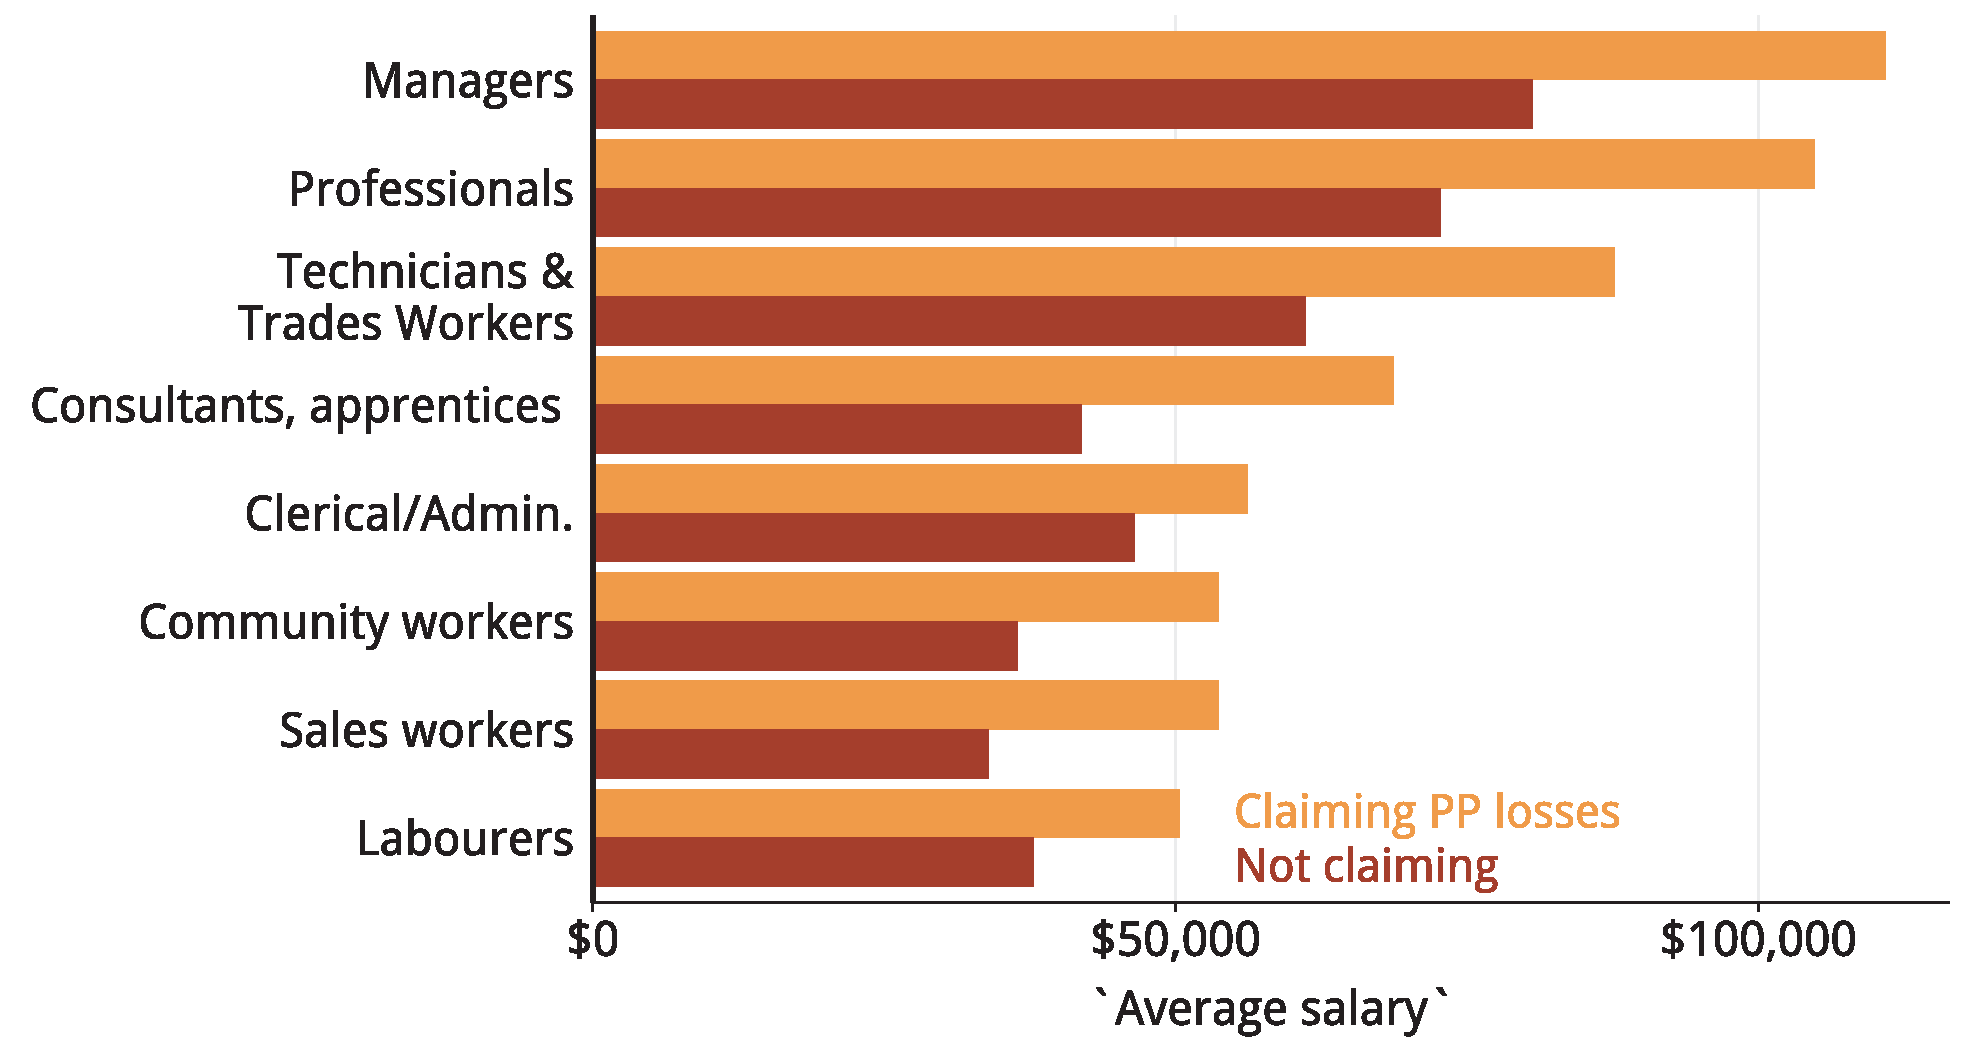
\includegraphics[width=1.2\columnwidth, right]{CGT-NG-atlas/b5-palatino-atlas/PP-losers-salary-comparison-horiz-bar-1.pdf}
\source{\textcite{ATO2016SampleFile1314}.}
\end{figure}

\begin{figure}[t]
\caption*{\dots\ and claim more often}
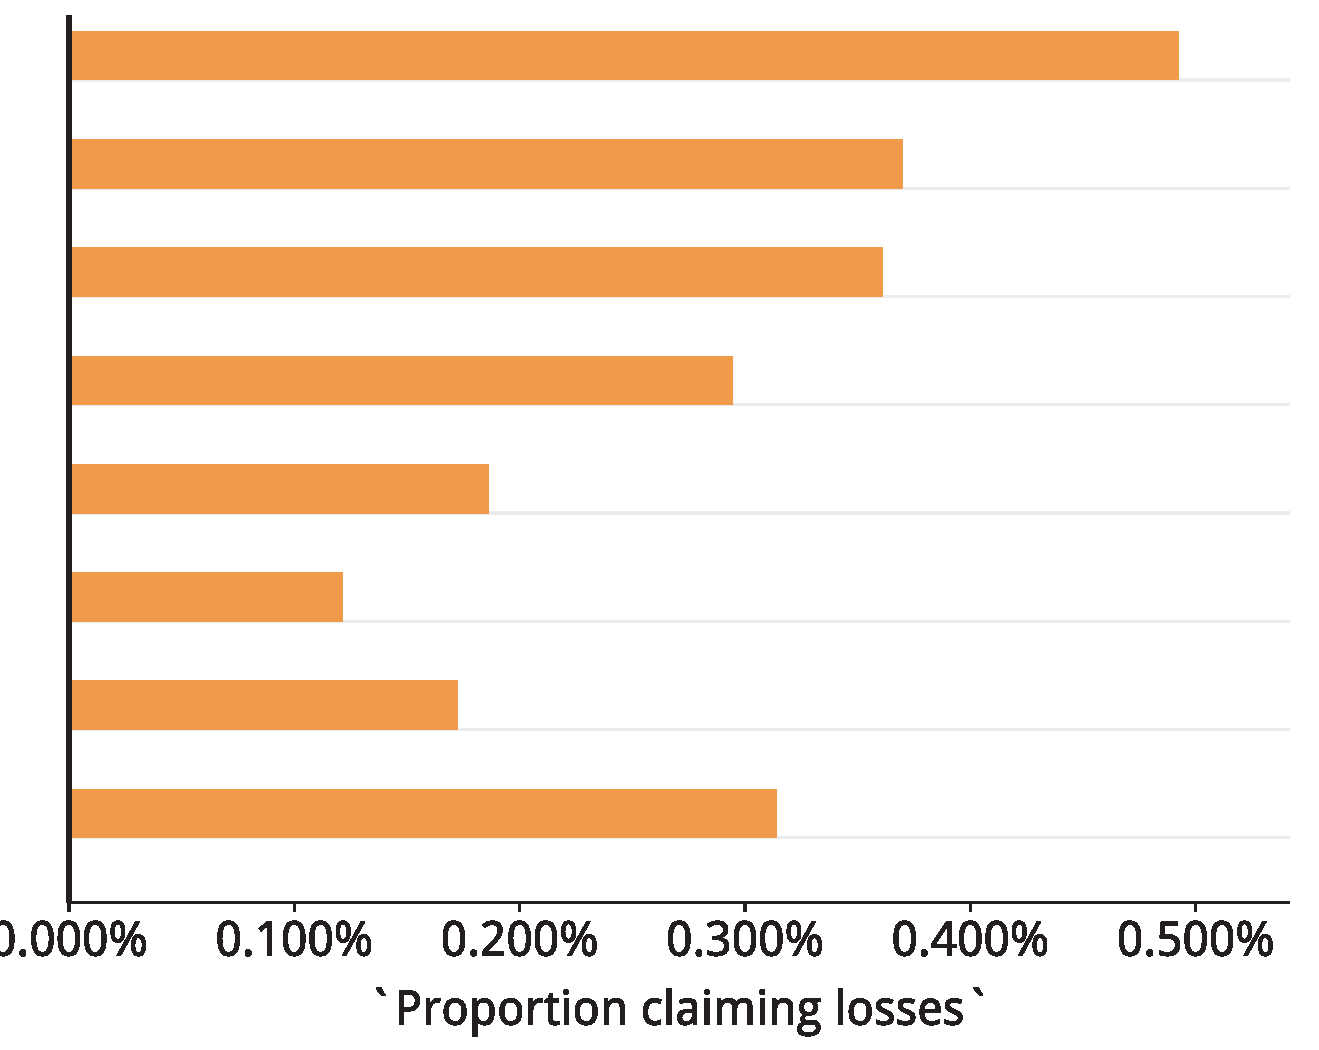
\includegraphics[width=0.8\columnwidth]{CGT-NG-atlas/b5-palatino-atlas/Proportions-PP-losses-1.pdf}
\caption*{}
% \source{\textcite{ATO2016SampleFile1314}.}
\end{figure}

At present there are more restrictions on deducting business losses than there are on deducting losses from investments. Sole traders and participants in a partnership can write off losses from these business activities against unrelated income (including wages) only if they meet a variety of conditions that generally exclude activities that make persistent losses.\footnote{If the business is a primary production business or a professional arts business, losses can only be deducted if other income (such as wages and salaries) is less than \$40,000 a year; for other businesses, losses can only be deducted if wage and salary income is less than \$250,000, and if the business has top-line income of at least \$20,000, made a profit in three of the previous 4 years, owns property worth at least \$500,000 used for a business activity, or uses other assets worth at least \$100,000: see \textcite{ATO2015OffsettingCurrentYearLosses}.} Losses for incorporated businesses cannot be written off against other income. 

The losses claimed are relatively small. In 2013-14 only 240,000 taxpayers claimed \$4 billion in business losses (compared to 1.2 million people claiming \$10 billion in losses on property).\label{insec:number-taxpayers-claiming-business-losses}

Business losses are readily distinguished from investment losses. Tax systems in other countries draw precisely this distinction.\footnote{See \stopifendnote{}\vref{footnote:passive-income}.} Other parts of Australia’s tax system already apply different tax treatments to active and passive investments – for example, rules governing the availability of capital gains tax concessions for small business.\footnote{Under the active asset test, small business can only claim CGT concessions for those assets used or held ready to use in the course of carrying on a business. See: \textcite{ATO2015ActiveAssetTest}.} These rules are relatively easy to enforce,\footcite{Mather2016} so providing a different tax treatment for active assets should not raise large-scale concerns about avoidance. 

Allowing business losses to be deducted from general income recognises that small business owners, particularly in the early stages of a new business, may use their income from employment to fund their business losses. Working part-time may help some new business owners better manage the risks of starting a new business. The argument for retaining loss write-offs is to maintain the incentive for this type of ‘toe in the water’ entrepreneurship. 

However, many of the losses being claimed may not serve this policy purpose. About 40 per cent of business losses claimed are from primary production – animal or crop farming, vineyards or animal breeding, for example. About 53,000 taxpayers claimed \$1.6 billion in primary production losses – about \$30,000 per claimant. In all occupational categories, average salaries for those claiming primary production losses were substantially higher – between 20 and 65 per cent – than the average salaries for their occupation (\Vref{fig:PP-losses-by-salary}). This suggests primary production activity may often be more a lifestyle activity such as a hobby farm, than a sustainable business.


About 190,000 taxpayers claimed an average of \$13,000 of non farm business losses. It is likely that many of these people were individual contractors in fields related to their main job. Some of the losses may simply be taxpayers claiming lifestyle costs where they will be less scrutinised. 
That is because tax returns require less detail for costs claimed as part of running a business rather than in incurring wage and salary income (for example, travel costs do not need to be separately disclosed). 

Nevertheless, given the low costs and potentially meaningful benefits the best approach is probably to leave the current tax treatment for losses from unincorporated businesses in place. 
In other words, only losses from passive investments would be quarantined so they cannot be written off against wage and salary income. 
This approach is in place in the United States (\Vref{appendix:Intl-comparisons-tax-loss-deductibility}). 

\subsection{Budget impact}
Restricting negative gearing by quarantining loss deductions for passive investments would raise more tax revenue. How much depends on future housing prices and how long investors hold their assets.

For most investors, the changes will mainly affect the timing, not the amount, of tax deductions. The costs of property and share investments can still be deducted against future investment income, including any capital gains made after the asset is sold.

We estimate that quarantining losses for passive investments would increase income tax collections by \textbf{\$2~billion} a year in the short term. Over the medium term, accrued losses – losses not offset against recurrent investment income – will be deducted from capital gains. Assuming no change in investor behaviour, the additional tax revenue would stabilise at about \textbf{\$1.6~billion} a year.\footnote{The short-term costing is the amount of money that would be raised in year one of the policy change, assuming taxpayers had no other investment income in that year against which to offset losses. The longer term or steady state estimate reflects the fact that losses carried forward will be written off against positive investment income as it accrues for investors} 

If deductions were limited even more to the particular asset or asset class, income tax collections would rise a little more because investors would wait longer on average until they could realise their losses. 

These estimates do not take into account the effects of investors changing their behaviour in response to the policy change. Investments that make income losses are less attractive when the tax benefits are smaller. Negative gearing appeals largely because it can reduce taxes on wage income (\Cref{sec:negative-gearing-provides-a-widely-used-tax-shelter-on-wages}). Removing the tax incentive for highly leveraged investment should lead investors to shift toward income-producing assets and could therefore further increase income tax collections. On the other hand, if some investment properties are replaced by owner-occupied properties, less revenue will be collected, because no tax is paid on capital gains on the family home, or on the ‘imputed rent’ – the value of living in occupier-owned housing.

\section{Alternative policies for limiting negative gearing}
Our proposed policy of quarantining investment losses from wage and salary income would apply to losses from all passive investments regardless of the nature or the size of the investment. 

Others have proposed less universal changes. For example, Labor’s negative gearing policy would continue to allow unrestricted loss write-offs for new housing.\footcite{ALP2016PositivePlanHousing} It was reported in 2016 that the Coalition contemplated policies to cap loss deductions or limit the number of properties that could be negatively geared.\footcite{Coorey2016}  

These ‘halfway house’ policies are not ideal. The economic arguments for limiting negative gearing apply regardless of investment size or type. By limiting the changes some of the potential budgetary benefits are lost. And introducing differential tax treatments based on the size or type of investment further increases complexity and distorts investment decisions. 

Even so, limiting negative gearing to new properties or capping loss deductions at modest levels would only impose modest costs on the budget and the economy. These carve outs may be worthwhile if they make changes to negative gearing more politically palatable.

On the other hand, capping the number of properties that can be negatively geared or setting a high threshold for loss deductions, eliminate almost all the revenue gains from policy change while introducing additional distortions. 

\subsection{Limiting negative gearing only to new properties}
It would be possible to quarantine wage and salary income generally, but to allow losses on new properties to be deducted from wages and salaries. 

Proponents argue that this exemption will maintain the incentives for the provision of new housing.\footcite[][28]{McKellInstitute2015SwitchingGears}  But in practice it won’t make much difference: most of the tax benefits will be reflected in a one-off change in the price of land suitable for development. The supply of such land is not particularly responsive to price changes as \Cref{sec:Impact-new-development} shows. Therefore the value of special tax treatment for new development will mainly flow to landholders. 

In any case, the benefits of negative gearing on new properties only are likely to be small relative to the price of property and the cost of development – about 2 per cent of the property value.  Even if all of this benefit flowed to developers and purchasers, not to the owners of land suitable for development, there wouldn’t be much additional development activity. And of course the impact on overall housing supply would be smaller again because few additional properties are built in any year relative to the stock of existing properties.\footnote{Because a second purchaser will not be eligible to negatively gear the property, the total tax benefit will be the value of negative gearing for the average period that properties are held by their first purchaser. The annual benefit is around 0.4 per cent of the property value. Properties tend to stay negatively geared for around five years (see \Vref{footnote:number-years-for-NG}\stopifendnote{}).} 

Restricting tax benefits to a subset of investments, such as new housing, creates additional complexity and distorts investment choices. But the costs may not be high. Administrative issues such as how to define ‘new properties’ have already been addressed through government support schemes that target new property investments. These include first homebuyer’s grants and stamp duty concessions. 

There are clear political benefits to such an exemption.  It appeals to intuitions that tax benefits will produce more new housing, even if theory and history suggest that the effects will be small.  As the additional costs are low, it may be a political price worth paying.



\subsection{Capping loss deductions}
Capping the total amount of losses that can be deducted each year for negatively geared properties has been proposed as a way to curb the ‘excesses’ of negative gearing policy.\footnote{This was reported one of the policy alternatives considered by Treasurer Scott Morrison when he raised concerns about the ‘excesses’ of negative gearing. See: \textcite{Coorey2016}.}



Capping losses is politically attractive because fewer landlords will be affected by the policy. 
And the landlords affected are more likely to be high-income earners because those on high incomes claim much higher losses on average (\Vref{fig:NG-by-occup}). 

\begin{table}
\caption{Budgetary impact of caps to negative gearing}\label{tbl:cap-NG}
% latex table generated in R 3.2.5 by xtable 1.8-2 package
% Sun Apr 24 12:05:04 2016
\centering
\begin{tabularx}{0.80\linewidth}{rRR}
  \toprule
{\textbf{Threshold}} & {\textbf{Revenue impact (2015-16 billions)}} & {\textbf{Landlords affected (\%)}} \\ 
  \midrule
% $-$\$0 & \$2,367,161,951 & 750,916 & 37.5\% \\ 
  \$5,000 & \$$1.3$\phantom{0} &  20.0\% \\ 
  \$10,000 & \$$0.8$\phantom{0} &  10.4\% \\ 
  \$15,000 & \$$0.5$\phantom{0} &  5.8\% \\ 
  \$20,000 & \$$0.3$\phantom{0} & 3.4\% \\ 
  \$50,000 & \$$0.04$ & 0.4\% \\ 
   \bottomrule
\end{tabularx}
\tnotes{tbl:cap-NG}{Assumes that all net rental losses above the cap in a year cannot be written off against wage and salary income. That is, if the investor does not make other (positive) investment income in that year then the loss in excess of the cap cannot be claimed.}

\source{\gao\ \textcite{ATO2016SampleFile1314}.\hfill\null}
\end{table}

The budget impact will depend on the level of the cap, as set out in \Vref{tbl:cap-NG}. A cap on losses of \$20,000 or more would affect very few landlords, but make very little difference to the budget bottom line.

An alternative is to limit deductions. This could apply to all deductions including work-related expenses, interest costs, donations etc.\footnote{A universal cap on all deductions would ultimately impose a minimum effective rate of tax for high-income earners. See: \textcite[][61]{BCA2016}.}  This is beyond the scope of this report. 

\subsection{Limits on number of properties}
An alternative proposal would limit the number of properties on which investors are able to claim losses.\footnote{According to reports, this policy option was also considered by the Treasurer in 2016. See: \textcite{Coorey2016}.}  This option is unattractive. It is poorly targeted, would raise little, and would increase distortions in the housing market.

Only 28 per cent of landlords have two or more properties.\footnote{\textcites{ABS2015-Survey-of-income-and-housing-2013-14}{HILDA2015} Not all of these will be negatively geared, but it is reasonable to assume that the proportion of negatively geared landlords who own multiple properties is no higher than for other landlords.} A fraction of these would not be taxed as they would the ‘first property’ for a landlord. The relatively small number of taxpayers affected substantially reduces the potential budget gains. 

In any case, capping property numbers is a crude way to target ‘excessive’ negative gearing. Taxpayers can increase their deductions by purchasing fewer but more expensive properties. Consequently the policy will distort investment decisions by discouraging investors from buying more affordable properties. 

\section{Summarising impact of proposed negative gearing and CGT changes}\label{sec:Summarizing-impact-proposed-NG-and-CGT}
Our preferred policy is to reduce the CGT discount to 25 per cent and to limit negative gearing by quarantining all passive investment losses.

As well as raising more than \$6~billion a year, the changes will reduce (though not eliminate) distortions in investment choices toward debt-financing of investment. Effective tax rates will increase a bit more for highly leveraged investors because they lose some of the tax benefits of upfront loss write-offs (\Vref{fig:16}). However, effective tax rates will remain lower for this group because they still eventually write off their losses at a tax rate higher than they pay on gains.  

\begin{figure}
\captionwithunits{Proposals increase effective tax rates, particularly for heavily geared properties}{Real effective marginal tax rates}\label{fig:16}
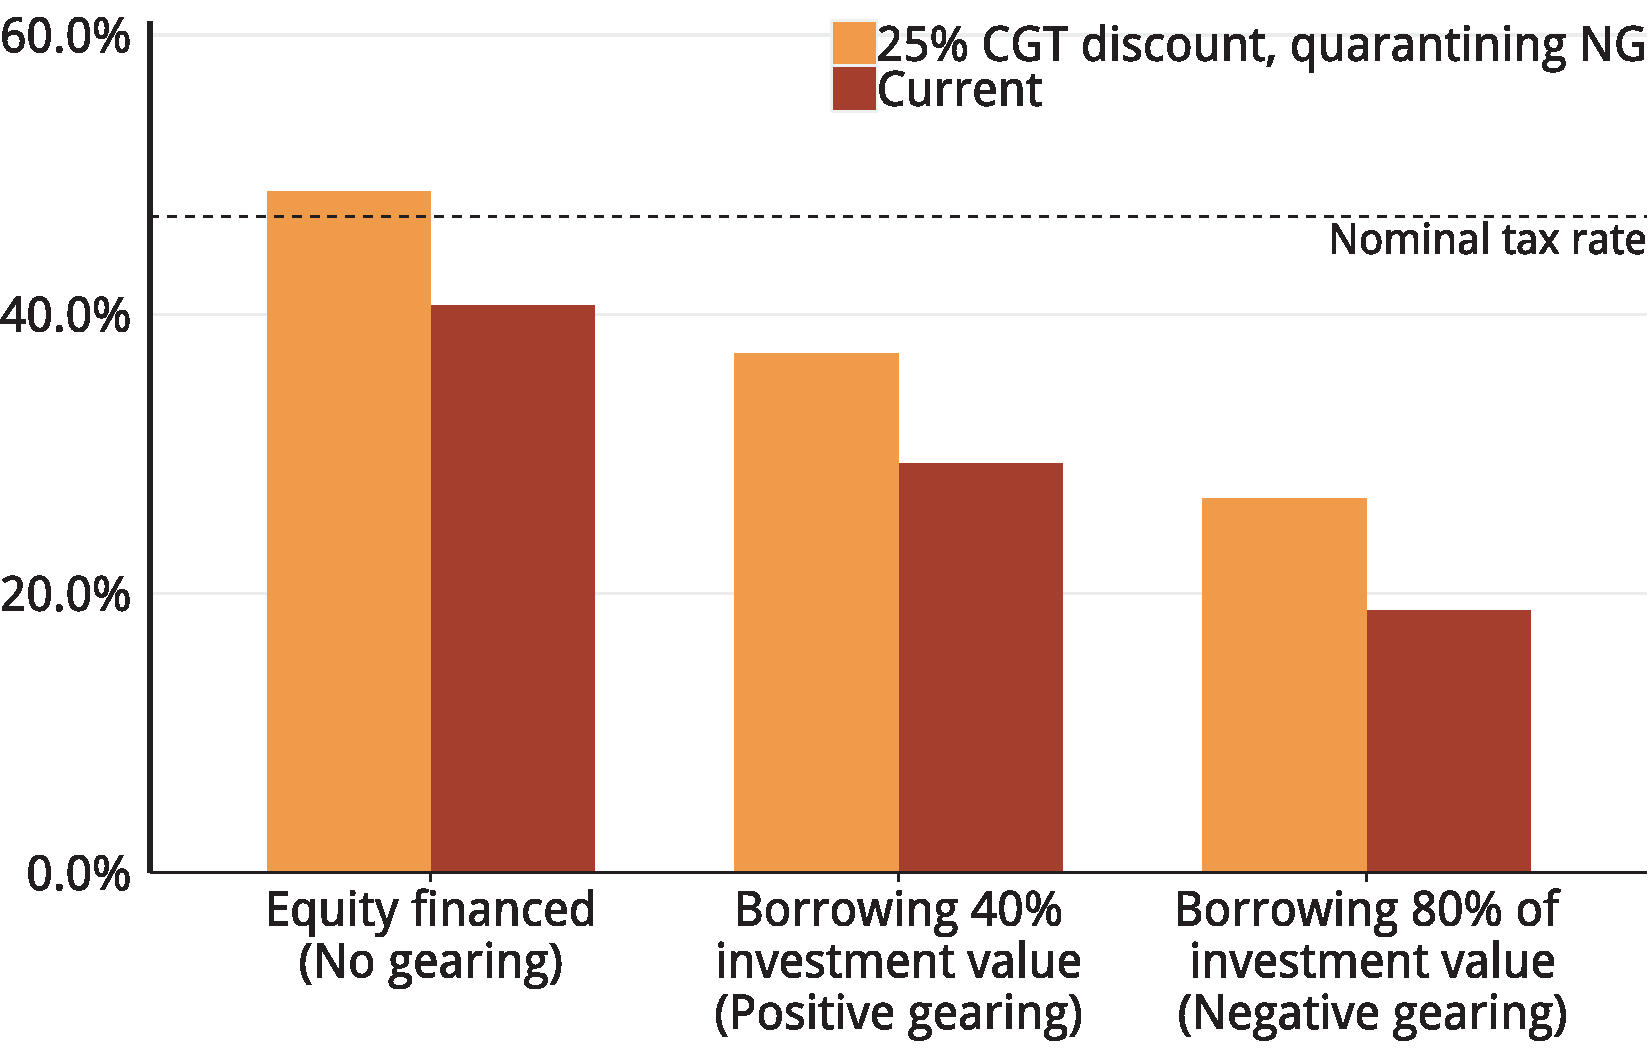
\includegraphics[width=\columnwidth]{CGT-NG-atlas/b5-atlas/CGT-fig16-1.pdf}
\fnotes{fig:16}{See \Vref{tbl:EMTR-savings-assumptions}.}
\source{Grattan analysis.}
\end{figure}

The changes will improve affordability and price stability in property markets, while not unduly affecting the supply of rental properties or incentives to save.

\section{A longer term reform objective}\label{sec:A-longer-term-reform-objective}
In an ideal world, as envisaged by the Henry Review, tax rates would be consistent across different types of savings unless there was a good policy reason for the difference (such as lower taxes on superannuation contributions and owner-occupied housing – see \Cref{subsubsec:reducing-distortion-between-investment-choices}). 

The Henry Review proposed aligning the tax treatment of savings better both by increasing taxes on capital gains, and by reducing taxes on recurrent income and bank deposits. These changes would further reduce distortions in investment choices. They would reduce the difference in returns between geared and ungeared investments, and remove the tax penalty for savings in bank deposits. However, providing these additional tax discounts would strain the budget and is implausible given current fiscal constraints,\footcites{Daley2015} even if it remains a longer term reform objective.

\chapter{Transition arrangements}
Transition arrangements for changes in the tax treatment of investments could help minimise price shocks in asset markets and make reforms easier to sell. 

Changes to both capital gains and negative gearing could be phased-in over time. Grandfathering arrangements for existing investors is an alternative. Grandfathering would raise a host of problems for capital gains tax but has fewer drawbacks for negative gearing. 

Phasing-in tax changes and grandfathering would both significantly reduce the revenue from the policy change in the initial years. 

\section{Phase-in reforms}
Changes to the current capital gains discount or negative gearing regimes could be phased-in over a number of years, to prevent a rush of investors selling property before the new legislation came into force. For example, under a five-year phase-in, the capital gains discount could be reduced to 45 per cent in the first year, and then reduced by five percentage points each year until 75 per cent of capital gains are taxed. 

Changes to negative gearing could also be phased in. For example, taxpayers might be allowed to claim only 80 per cent of their losses against wage and salary income in the first year (the remainder capitalised against any future capital gain), and the twenty percentage points less each year until no losses are claimed against wage and salary income.

In both cases, the phase-in would provide investors with time to reorganise their affairs to adjust to the new regime.

\section{Grandfathering existing arrangements}
Another option would be to grandfather existing arrangements. Those who purchased assets before capital gains tax reform was implemented could still claim the capital gains tax discount, even if they sell the assets several years afterwards. Similarly, those who purchased assets before negative gearing reform, could continue to claim all of their losses against their wage and salary income until the asset was sold.

The most powerful argument for grandfathering is pragmatic: to defuse vociferous opposition from those who benefit from the current arrangements.

But for capital gains tax changes, grandfathering causes a number of problems: it adds to complexity, reduces liquidity, and treats new investors – particularly younger investors – unfairly.

Applying different tax treatments to investments depending on when they were acquired makes the tax system much more complex. Because investors can hold assets for decades, these dual tax arrangements are long-lived.  For example, the decision to grandfather the capital gains tax-free status for assets purchased before 1986 still contributes to the complexity of our capital gains tax regime, three decades later.\footcite[][75]{HenryTaxReview2010} 

Grandfathering arrangements reduce liquidity because investors have substantial incentives to retain whichever assets they purchased before the reform was implemented. They will be reluctant to buy and sell because the after-tax returns on the assets bought earlier will be higher. Such a drag on liquidity is economically inefficient because it encourages investors to hold assets even when others could extract a higher return from them. 

Grandfathering also exacerbates intergenerational inequality.\footcite{DaleyWoodWeidmannEtAl2014}  Those who own assets before the reforms – more likely those who are older\footcite[][14]{DaleyWoodWeidmannEtAl2014}  – earn higher after-tax returns than those who start to build wealth later on. 

For negative gearing, grandfathering raises fewer concerns. The fact that properties usually become positively geared over time, normally within five years (\Cref{subsec:In-principle-losses-should-not-be-deducted-from-salary}), provides a natural sunset to any grandfathering arrangements. Any issues around the complexity or unfairness of dual arrangements will inevitably be short-lived. 

Nevertheless, given the competing considerations, phase-in would be a better transition than grandfathering. It would be less complex, have less immediate impact on prices, and younger investors would be treated more fairly. Investors should not have too many concerns as the phase-in proposed would give them ample time to reorder their affairs.
















% citations
%\nocite{R-ggrepel,R-testthat,R-taxstats,R-magrittr,R-tidyr,R-devtools,R-expm,R-Matrix,R-Hmisc,R-Formula,R-survival,R-lattice,R-foreign,R-survey,R-zoo,R-httr,R-rsdmx,R-readr,R-openxlsx,R-readxl,R-xtable,R-grattan,R-directlabels,R-scales,R-ggplot2,R-gridExtra,R-dplyr,R-data.table,R-devEMF,R-knitr}


%\printendnotes[grattanEndnotes]
\makeatletter
\@openrightfalse
\makeatother

\begin{subappendices}

\cleardoubleevenstandardpage
\chapter{Capital gains tax and asset lock-in}\label{appendix:CGT-asset-lock-in}
One reason often provided for lower taxes on capital gains is to reduce ``asset lock-in''. If investors are less likely to realise gains when tax rates are higher than increasing taxes on gains could actually reduce tax collections in the short to medium term. But the empirical evidence of lock-in in not settled. In Australia, the primary driver of asset lock-in appears to be people waiting until retirement to sell their assets. This incentive is still strong even with a 50 per cent discount. 

\section{Why does asset lock-in occur?}
Asset lock-in occurs because taxes are only paid when gains are realised. This provides an incentive for investors to hold on to assets with large accumulated gains.\footcite{Burman2009}  In effect, the investor seeks to maintain the implicit interest free loan on accrued gains. Crystallising a capital gain is only worthwhile if an investor can achieve a materially higher return elsewhere, or if they want the resources for consumption (\Vref{box:CGT-asset-lock-in}).\footcite[][12]{Ingles2009a}   

Lock-in can discourage investors from moving their money to the investments with the highest pre-tax returns, so assets do not always go to their highest value use.\footcite{Lindsey1987}  Lock-in effects are most significant from a whole of economy perspective, if they constrain financing of profitable investments.\footcites{OECD2006TaxationOfCapitalGains}{Johnson2008}  


Australia’s open capital markets and generous capital gains tax regime for non-residents, reduce the danger that worthwhile projects will not get access to capital because of lock-in.\footnote{Non-resident investors in Australian shares are generally not subject to Australian capital gains tax (see: \Act{Income Tax Assessment Act 1936}{Cth}, s 136-25). } 

\begin{smallbox}[!hp]{Capital gains tax and asset lock-in}{box:CGT-asset-lock-in}
The tax treatment of capital gains can deter investors from taking up otherwise profitable investment opportunities. 



Suppose Hayley, an investor in the top tax bracket purchases a house for \$700,000 and holds it for 10 years. During that time the market price of the house increases to \$1,000,000. She makes a net rental return of 5~per cent a year, so her  final income is \$50,000. 

If she were to sell the house she would crystallise the \$300,000 in gains, paying tax on 50~per cent of the gains at her marginal tax rate of 49~per cent (\$73,500). This would leave her with around \$926,500 from the sale: \$226,500 in net gains and her initial investment of \$700,000. 

The sale will only be worthwhile if Hayley can find an alternative property that yields more than her current rental income of \$50,000  with the same opportunity for capital gains. With her \$926,500 sale proceeds she would need to find a property with net rental return of more than 5.4~per cent a year. 

Properties with rental yields below 5.4~per cent but higher than her current 5 would not be attractive because realising the tax liability on her current property erodes her capital base for investment.  

The higher the tax rate on capital gains the less willing she will be to realise gains to pursue new investment opportunities. If capital gains were taxed in full, rather than with a 50 per cent discount, her hurdle rate for the new investment would be 5.9~per cent.
\end{smallbox}
\clearpage

\section{Impact of lock-in on tax collections}

The long-term effect of asset lock-in on capital gains tax receipts has not been settled. The first paper to delineate the effects of tax changes on capital gains realisations over time, estimated that the long run responses to tax changes are significantly smaller that the immediate responses.\footnote{\textcite{BurmanRandolph1994} This finding helped reconcile the high estimated elasticities from cross-sectional studies (which measure transitory effects) and the low estimates from time series studies (which measure permanent effects).} 

More recent research by \textcite{CBO2012CapitalGainsTaxElasticity} found much higher persistent lock-in effects overall, but also that the size of the effect depends on the entity: mutual funds are almost entirely unresponsive to higher taxes, whereas pass-through entities (such as partnerships, trusts and limited liability companies) were much more likely to hold on to assets.

A key cause of lock-in is investors waiting until they are retired – and their taxable incomes are low – to realise gains. This reduces the average tax rate they pay on gains. The probability of a landlord selling a property increases by over 20 percentage points once they retire.\footcite{WoodOng2010}  And we can see the ‘retirement realisation effect’ in the patterns of capital gains realisation by age. Those over 65 have much higher average realisation of gains, regardless of their income level (\Vref{fig:CGT-by-age-income}). 

The other important cause of lock-in is the fact that capital gains are disregarded on death. Passing assets to a beneficiary is not regarded as an ‘event’ that triggers a capital gains tax liability. So by passing on assets to heirs, capital gains taxes can de deferred indefinitely. 

Ultimately, the best way to reduce asset lock-in is to tax gains on an accruals basis, with interest charges on the deferred tax.\footcites[][11--14]{Burman2009}[][12]{Ingles2009a}  Requiring tax be paid on notional gains an annual basis would raise substantial cash flow issues for many investors. 

Applying interest charges to the deferred tax would reduce the incentive to hold on to gains to reduce the tax burden. To date, annual asset revaluations have been considered impractical and beset with administrative difficulties.  But such valuations can be done easily for shares and to a lesser extent property (which is already revalued in most states every one or two years for the purposes of levying council rates).\FOOTNOTE{See \Vref{sec:PROP-5-2}.}  The Henry review flagged that such an accruals approach to capital gains may become more feasible as technology improves.\footcite[][64]{HenryTaxReview2010} 

% For longtable.
%\flushcolsend

\cleardoubleevenstandardpage
\chapter{Effective tax rates by investment return and tax bracket}\label{appendix:EMTRs}
Effective tax rates measure the tax paid on investment returns as a share of the pre-tax returns. Effective tax rates vary by the investor’s tax rate and the level of returns. When looking at effective tax rate on real returns (returns adjusted for inflation) or on `excess returns' (returns above the risk free rate) the level of inflation and the returns will also affect the effective tax rate paid by the investor. 

\Vref{fig:EMTR-savings} presents effective rates for two different return scenarios for an investor in the 47\,c tax bracket. \Vref{tbl:Real-EMTR-appendix} presents calculations for a broader range of return scenarios and investor tax brackets. 




\begin{table*}
\centering
\captionsetup{justification=centering}
\caption[Effective marginal tax rates for a rental property]{Effective marginal tax rates for a rental property}\label{tbl:Real-EMTR-appendix}
\newcolumntype{Q}{@{}l@{}}
% latex table generated in R 3.2.5 by xtable 1.8-2 package
% Mon Apr 25 19:50:50 2016
\makebox[\textwidth]{\begin{tabular}{Qlllrrrrr}
  \toprule
   &  &  &  & \multicolumn{5}{c}{\textbf{Nominal annual capital gain}}\\
 \cmidrule(lr){5-9}
 \textbf{\phantom{.}} & \textbf{MTR} & \textbf{Return type} & \textbf{CGT treatment} & \textbf{4\%} & \textbf{5\%} & \textbf{6\%} & \textbf{8\%} & \textbf{10\%}\\
 \midrule
 & $34.5$\% & real & 50\% discount & $33.9$ & $29.4$ & $26.2$ & $21.7$ & $18.7$ \\ 
   &  &  & Indexed & $34.3$ & $32.6$ & $31.1$ & $28.5$ & $26.2$ \\ 
   &  &  & 25\% discount & $39.6$ & $35.0$ & $31.7$ & $26.9$ & $23.6$ \\ 
   &  &  & 0\% discount & $45.5$ & $40.9$ & $37.4$ & $32.4$ & $28.8$ \\ 
   &\phantom{.}\\[-9pt] 
   &  & excess & 50\% discount & $61.0$ & $46.2$ & $37.8$ & $28.4$ & $23.1$ \\ 
   &  &  & Indexed & $61.7$ & $51.2$ & $44.9$ & $37.2$ & $32.4$ \\ 
   &  &  & 25\% discount & $71.3$ & $55.1$ & $45.8$ & $35.2$ & $29.1$ \\ 
   &  &  & 0\% discount & $82.0$ & $64.3$ & $54.1$ & $42.4$ & $35.5$ \\ 
   &\phantom{.}\\[-6pt]
   & $39.0$\% & real & 50\% discount & $38.5$ & $33.4$ & $29.8$ & $24.7$ & $21.3$ \\ 
   &  &  & Indexed & $38.8$ & $37.0$ & $35.4$ & $32.5$ & $30.0$ \\ 
   &  &  & 25\% discount & $45.1$ & $39.9$ & $36.1$ & $30.7$ & $27.0$ \\ 
   &  &  & 0\% discount & $51.9$ & $46.7$ & $42.8$ & $37.1$ & $33.1$ \\ 
   &\phantom{.}\\[-9pt] &  & excess & 50\% discount & $69.2$ & $52.5$ & $43.0$ & $32.3$ & $26.3$ \\ 
   &  &  & Indexed & $69.8$ & $58.1$ & $51.1$ & $42.5$ & $37.1$ \\ 
   &  &  & 25\% discount & $81.1$ & $62.7$ & $52.2$ & $40.2$ & $33.3$ \\ 
   &  &  & 0\% discount & $93.5$ & $73.4$ & $61.9$ & $48.6$ & $40.9$ \\ 
   &\phantom{.}\\[-6pt]
   & $47.0$\% & real & 50\% discount & $46.7$ & $40.6$ & $36.2$ & $30.1$ & $26.0$ \\ 
   &  &  & Indexed & $46.8$ & $44.8$ & $43.1$ & $39.9$ & $37.1$ \\ 
   &  &  & 25\% discount & $54.9$ & $48.8$ & $44.2$ & $37.7$ & $33.2$ \\ 
   &  &  & 0\% discount & $63.6$ & $57.4$ & $52.8$ & $46.0$ & $41.1$ \\ 
   &\phantom{.}\\[-9pt]
   &  & excess & 50\% discount & $84.0$ & $63.8$ & $52.3$ & $39.4$ & $32.1$ \\ 
   &  &  & Indexed & $84.2$ & $70.5$ & $62.2$ & $52.2$ & $45.8$ \\ 
   &  &  & 25\% discount & $98.9$ & $76.6$ & $63.8$ & $49.3$ & $41.0$ \\ 
   &  &  & 0\% discount & 1$14.5$ & $90.2$ & $76.2$ & $60.2$ & $50.8$ \\ 
   \bottomrule
\end{tabular}}

\begin{tabular}{l@{}p{0.9\textwidth}}
{\footnotesize Notes:\hspace{1em}} & {\footnotesize Inflation 2.5\%. Property earns 3\%\ nominal rent in addition to the capital growth and which is reinvested in the property till maturity. Risk free rate 4.5\%. Property is held for 15 years then disposed and capital gain realized without losses.}
\end{tabular}
\end{table*}
\renewcommand{\arraystretch}{1.0}
\normalsize


\chapter{International comparisons of capital gains tax}\label{appendix:Intl-comparisons-of-CGT}
Internationally, there are a range of approaches to taxing capital gains. Most countries offer some form of tax discount for capital income but the amount of the discount and the holding period to qualify vary widely. Contrary to the claims of some, taxes on capital gains are more concessional than in many other OECD countries 

\newcommand{\cella}[1]{#1}
\newcommand{\cellb}[1]{#1}
\newcommand{\cellc}[1]{#1}
\newcommand{\celld}[1]{#1}

% \newcommand{\cella}[1]{{\cellcolor{Color2}\makecell[tr]{#1}}}
% \newcommand{\cellb}[1]{{\cellcolor{Color3}\makecell[tr]{#1}}}
% \newcommand{\cellc}[1]{\cellcolor{Color4}{\makecell[tr]{#1}}}
% \newcommand{\celld}[1]{\cellcolor{Color5}\makecell[tr]{#1}}


\cleardoubleevenstandardpage
\thispagestyle{empty}
\enlargethispage{20pt}
\begin{table}
\captionsetup{justification=centering, skip=0pt}
\caption{Tax treatment of capital gains in property, by country}
\vspace*{-2ex}%
\makebox[\textwidth]{%
\renewcommand{\arraystretch}{0.99}%
\begin{tabular}[t]{>{\footnotesize}l>{\raggedleft\footnotesize}p{6.35cm}>{\raggedleft\footnotesize}p{1.20cm}>{\footnotesize}r>{\footnotesize\raggedleft\arraybackslash}p{1.40cm}}
\toprule
 %                     & \multicolumn{2}{c}{\textbf{Property}}                                                                                                                        & \\
 %\cmidrule(lr){2-3}
 \textbf{Country}     & \textbf{CGT treatment}                                   & \textbf{Holding test} & \textbf{Top MTR} & \textbf{Adj for \mbox{inflation?}} \\
 \midrule
 \textbf{Australia}   & {50\%\ exempt, rest at MTR}                              & {1\,yr}               & 47               & N\\
 \textbf{Austria}     & {Progressive rise to 50\% from 10-35 years, rest at MTR} & {10-35\,yr}           & {50}             & {N} \\
 \textbf{Belgium}     & {Exempt}                                                 & {5-8\,yr}             & {45.3}           & {N} \\
 \textbf{Canada}      & 50\% exempt, rest at MTR                                 & --                    & 49.5             & N \\
 \textbf{Chile}       & Exempt                                                   & 1\,yr                 & 40               & Y \\
 \textbf{Czech Rep}   & Exempt                                                   & 5\,yr                 & 20.1             & N \\
 \textbf{Denmark}     & MTR                                                      & --                    & \textit{{55.8}}  & N\\
 \textbf{Estonia}     & MTR                                                      & --                    & \textit{19.7}    & N \\
 \textbf{Finland}     & MTR on (CG $-$ 20\%) of sale price $<$\,10\,yrs          & {10\,yr}              & {49.1}           & {N} \\[-1pt]
                      & MTR on (CG $-$ 40\%) of sale price $<$\,10\,yrs          &                       &                  & \\[4pt]
 \textbf{France}      & Progressive rise to full exemption from 5-30\,yrs        & 5-30\,yr              & 54               & N \\
 \textbf{Germany}     & Exempt                                                   & 10\,yr                & 47.5             & N \\
 \textbf{Greece}      & Exempt unless bought for resale                          & --                    & 46               & N \\
 \textbf{Hungary}     & Exempt                                                   & 15\,yr                & 16               & N \\
 \textbf{Iceland}     & MTR                                                      & --                    & 44.4             & N \\
 \textbf{Ireland}     & CGT rate 30\%, fixed amount deductible                   & {--}                  & 47               & N \\
 \textbf{Israel}      & CGT rate 25\%                                            & --                    & 50               & Y \\
 \textbf{Italy}       & Exempt                                                   & 5\,yr                 & 48.8             & N \\
 \textbf{Japan}       & CGT rate 20\%                                            & 5\,yr                 & 56.6             & N \\
 \textbf{Korea}       & 30\% exempt, rest at MTR                                 & 10\,yr                & 39.4             & N \\
 \textbf{Luxembourg}  & CGT rate 10\%                                            & 2\,yr                 & 43.6             & N \\
 \textbf{Mexico}      & MTR                                                      & --                    & 35               & Y \\
 \textbf{Netherlands} & {{No realisation tax, annual tax @ deemed 30\%}}         & --                    & 49.2             & N \\
 \textbf{New Zealand} & {Exempt unless bought for resale}                        & --                    & 33               & N\\
 \textbf{Norway}      & MTR                                                      & --                    & 39               & N \\
 \textbf{Poland}      & {Exempt}                                                 & {5\,yr}               & {20.9}           & {N} \\
 \textbf{Portugal}    & 50\% exempt, rest at MTR                                 & 2\,yr                 & 50.3             & Y \\
 \textbf{Slovak Rep}  & Exempt                                                   & 5\,yr                 & 21.7             & N \\
 \textbf{Slovenia}    & Progressive exemption                                    & 20\,yr                & 39               & N \\
 \textbf{Spain}       & MTR                                                      & --                    & 46               & Y \\
 \textbf{Sweden}      & CGT rate 30\%                                            & --                    & 56.9             & N \\
 \textbf{Switzerland} & Exempt unless bought for resale                          & --                    & 36.1             & N \\
 \textbf{Turkey}      & 10\% exempt, rest at MTR                                 & 5\,yr                 & 35.8             & N \\
 \textbf{UK}          & CGT rate 18/28\%, fixed amount deductible                & --                    & 45               & N \\
 {\textbf{US}}        & Improvements (MTR with 25\% cap)                         & {1\,yr}               & {46.3}           & {N} \\
                      & land value increase (20\% CGT)                           &                       &                  & \\
                      & residual (20\% CGT)                                      &                       &                  & \\
\bottomrule
\end{tabular}}
\end{table}

\begin{table}
\captionsetup{justification=centering, skip=0pt}
\caption{Tax treatment of capital gains in shares, by country}%
\vspace*{-2ex}
\makebox[\textwidth]{%
\renewcommand{\arraystretch}{0.99}%
\begin{tabular}[t]{>{\footnotesize}l>{\raggedleft\footnotesize}p{6.30cm}>{\raggedleft\footnotesize}p{1.20cm}>{\footnotesize}r>{\footnotesize\raggedleft\arraybackslash}p{1.40cm}}
\toprule
 %                     & \multicolumn{2}{c}{\footnotesize\textbf{Shares}}                                                                                                                        & \\
 %\cmidrule(lr){2-3}
 \textbf{Country}     & \textbf{CGT treatment}                                                   & \textbf{Holding test} & \textbf{Top MTR} & \textbf{Adj for \mbox{inflation?}} \\
 \midrule
 \textbf{Australia}   & {50\%\ exempt, rest at MTR}                                              & {1\,yr}               & 47               & N\\
 \textbf{Austria}     & 25\% exempt, rest at MTR                 								 & --           & {50}             & {N} \\
 \textbf{Belgium}     & {Exempt}                                                                 & --             & {45.3}           & {N} \\
 \textbf{Canada}      & 50\% exempt, rest at MTR                                                 & --                    & 49.5             & N \\
 \textbf{Chile}       & Exempt                                                                   & 1\,yr                   & 40               & Y \\
 \textbf{Czech Rep}   & Exempt                                                                   & 0.5\,yr                   & 20.1             & N \\
 \textbf{Denmark}     & {{MTR}} & --                                                & \textit{{55.8}}       & N\\
 \textbf{Estonia}     & {{MTR}} & --                                              & \textit{19.7}         & N \\
 \textbf{Finland}     & MTR, with deductible amounts                       						& {10\,yr}                & {49.1}           & {N} \\
 %                     & 													                      &                       &                  & \\[4pt]
 \textbf{France}      & MTR                          											& --               & 54               & N \\
 \textbf{Germany}     & 26\% exempt, rest at MTR                                                                   & --                  & 47.5             & N \\
 \textbf{Greece}      & Exempt unless bought for resale                                          & --                    & 46               & N \\
 \textbf{Hungary}     & Exempt                                                                   & 5\,yr                  & 16               & N \\
 \textbf{Iceland}     & MTR                                            & --  & 44.4 & N \\
 \textbf{Ireland}     & MTR                                   & {--}                  & 47               & N \\
 \textbf{Israel}      & MTR                                                           & --                    & 50               & Y \\
 \textbf{Italy}       & CGT rate 20\%                                                                & --                  & 48.8             & N \\
 \textbf{Japan}       & CGT rate 10\%                                                            & --                   & 56.6             & N \\
 \textbf{Korea}       & Exempt                                                 & --                  & 39.4             & N \\
 \textbf{Luxembourg}  & MTR, fixed rate deductible                                                            & 0.5\,yr                   & 43.6             & N \\
 \textbf{Mexico}      & Exempt                                                                      & --                    & 35               & Y \\
 \textbf{Netherlands} & {{No realisation tax, annual tax @ deemed 30\%}} & -- & 49.2                  & N \\
 \textbf{New Zealand} & {Exempt unless bought for resale}     & --                 & 33                    & N\\
 \textbf{Norway}      & {{MTR}} & --                                               & 39                    & N \\
 \textbf{Poland}      & {CGT rate 19\%}                                                                 & --                 & {20.9}           & {N} \\
 \textbf{Portugal}    & 25\% exempt, rest at MTR                                                 & --                   & 50.3             & Y \\
 \textbf{Slovak Rep}  & MTR, fixed rate deductible                                                                   & --                   & 21.7             & N \\
 \textbf{Slovenia}    & CGT rate 5\%                                                    & 20\,yr                  & 39               & N \\
 \textbf{Spain}       & MTR                                                                      & --                    & 46               & Y \\
 \textbf{Sweden}      & CGT rate 30\%                                                            & --                    & 56.9             & N \\
 \textbf{Switzerland} & Exempt unless bought for resale                                          & --                    & 36.1             & N \\
 \textbf{Turkey}      & 10\% exempt, rest at MTR                                                 & 1\,yr                   & 35.8             & N \\
 \textbf{UK}          & CGT rate 18/28\%, fixed amount deductible                                & --                    & 45               & N \\
 {\textbf{US}}        & MTR                                         & {1\,yr}                 & {46.3}           & {N} \\
\bottomrule
\end{tabular}}
\end{table}

\renewcommand{\arraystretch}{1.0}
\normalsize

\chapter{International comparisons of tax loss deductibility\label{appendix:CGT-C}\label{appendix:Intl-comparisons-tax-loss-deductibility}}
Australia’s tax treatment of investment losses is more generous than most comparable countries. Most countries impose some limits on deductibility against wage and salary income (\Cref{tbl:CGT-5}).%

\afterpage{%
\thispagestyle{empty}}
\renewcommand{\arraystretch}{1.15}


% \begin{tabularx}{145mm}{>{\footnotesize\bfseries}l@{}>{\footnotesize\raggedleft}p{1.75cm}>{\footnotesize\raggedright}X>{\footnotesize\raggedleft}p{1.95cm}>{\footnotesize\RaggedRight\arraybackslash}X}
\begin{longtable}[r]{>{\footnotesize\bfseries}l@{}>{\footnotesize\raggedleft}p{1.75cm}>{\footnotesize\raggedright}p{3.00cm}>{\footnotesize\raggedleft}p{1.95cm}>{\footnotesize\raggedright\arraybackslash}p{3.22cm}}
\captionsetup{justification=centering}
\caption{Tax treatment of property investments by country\label{tbl:CGT-5}} \\
    \toprule
    \textbf{Country} & \textbf{Interest \mbox{deductions?}} & \textbf{Notes} & \textbf{Negative gearing?} & \textbf{Notes} \\
    \midrule 
	\endfirsthead
    \toprule
    \textbf{Country} & \textbf{Interest \mbox{deductions?}} & \textbf{Notes} & \textbf{Negative gearing?} & \textbf{Notes} \\
    \midrule 
    \endhead
    \bottomrule
    \endfoot
    Australia & Yes   &       & Yes   & Cash and depreciation expenses can be deducted against any other income \\

    Canada & Yes   & For interest expenses that are used to generate income. & Limited & Only cash expenses, not depreciation. Subject to a ‘reasonable expectations of profits test’. \\
    {France} & {Yes} &  & {Limited} & {Allowed up to a set limit and interest costs may not exceed gross rent} \\
          &       &       &       &  \\
    Germany & No    &       & Yes   &  \\
    Netherlands & No    &       & No    & Not possible. Taxation of investments based on an assumed yield of 4\%. \\
    NZ & Yes   & Deductible at marginal tax rate & Yes   & All losses deductible against labour income at marginal tax rate \\
    Sweden & Yes   &       & Yes   & Only deductible against capital income, not against salary and wage income, due to dual income tax system \\
    Switzerland & Yes   & Tax paid on imputed rental income, net of interest and renovation costs & Limited &  \\
    UK & Limited & From 2017, the value of tax deductions for interest expenses related to investment properties to be limited, only deductible up to the basic level of income taxation & Limited & Rental losses can only be offset against other rental income, but losses can be carried forward and deducted from future rental income. \\
    US & Limited & Usually deductible, but limited to the amount of investment income generated; interest expenses over this amount can be carried forward to future years. & Limited & Rental property expenses cannot be deducted against unrelated labour income. Deductible from other ‘passive’ activities only (unless gross income is below \$150\,k, in which case a capped amount can be claimed). Excess losses are carried forward. \\
\end{longtable}


\FloatBarrier
\chapter{Colophon}
The report was originally woven with \LaTeX2e and R by \textbf{knitr}. 

\LaTeX2e{} is a document preparation system implemented as a macro package for Donald E.\ Knuth's \TeX{} typesetting program. \LaTeX{} was originally conceived by Leslie Lamport. 

R is a language and environment for statistical computing derived from the S programming language of John Chambers. R was created by Ross Ihaka and Robert Gentleman at the University of Auckland. 

\textbf{knitr} a general-purpose package for dynamic, literate report generation in R developed from Sweave. Yihui Xie is the author and developer of \textbf{knitr}. 

The authors are indebted to the creators.

\section{R session information}
The session info (via devtools) is printed \emph{infra}.




\begin{table}[!htb]
\centering
\captionsetup{justification=centering}
\caption{Platform}
% latex table generated in R 3.2.5 by xtable 1.8-2 package
% Sun Apr 24 12:05:14 2016
\begin{tabular}{rl}
  \toprule
 version & R version 3.2.5 (2016-04-14) \\ 
  system & x86\_64, mingw32 \\ 
  ui & RTerm \\ 
  language & (EN) \\ 
  collate & English\_Australia.1252 \\ 
  tz & Australia/Sydney \\ 
  date & 2016-04-24 \\ 
   \bottomrule
\end{tabular}
\end{table}

\clearpage


% latex table generated in R 3.2.5 by xtable 1.8-2 package
% Sun Apr 24 12:05:14 2016
% \afterpage{\enlargethispage{2\baselineskip}}
% \begin{addmargin*}[0em]{-2em}
\footnotesize
\renewcommand{\arraystretch}{1.1}
\begin{longtable}{lllll}
\captionsetup{justification=centering}
\caption{Packages} \\ 
  \toprule
{\textbf{package}} & {\textbf{*}} & {\textbf{version}} & {\textbf{date}} & {\textbf{source}} \\ 
  \hline 
\endhead 
\hline 
&\multicolumn{2}{l}{\footnotesize ${}^*$ attached} & \multicolumn{2}{r}{\footnotesize Continued on next page} 
\endfoot 
\endlastfoot 
acepack &  & 1.3-3.3 & 2013-05-03 & CRAN (R 3.2.3) \\ 
  assertthat &  & 0.1 & 2013-12-06 & CRAN (R 3.2.5) \\ 
  bitops &  & 1.0-6 & 2013-08-17 & CRAN (R 3.2.3) \\ 
  chron &  & 2.3-47 & 2015-06-24 & CRAN (R 3.2.5) \\ 
  cluster &  & 2.0.3 & 2015-07-21 & CRAN (R 3.2.5) \\ 
  codetools &  & 0.2-14 & 2015-07-15 & CRAN (R 3.2.5) \\ 
  colorspace &  & 1.2-6 & 2015-03-11 & CRAN (R 3.2.5) \\ 
  crayon &  & 1.3.1 & 2015-07-13 & CRAN (R 3.2.5) \\ 
  curl &  & 0.9.7 & 2016-04-10 & CRAN (R 3.2.5) \\ 
  data.table & * & 1.9.6 & 2015-09-19 & CRAN (R 3.2.5) \\ 
  DBI &  & 0.3.1 & 2014-09-24 & CRAN (R 3.2.5) \\ 
  devEMF & * & 2.0 & 2015-01-29 & CRAN (R 3.2.3) \\ 
  devtools & * & 1.11.0 & 2016-04-12 & CRAN (R 3.2.5) \\ 
  digest &  & 0.6.9 & 2016-01-08 & CRAN (R 3.2.5) \\ 
  directlabels & * & 2015.12.16 & 2015-12-18 & CRAN (R 3.2.5) \\ 
  dplyr & * & 0.4.3 & 2015-09-01 & CRAN (R 3.2.5) \\ 
  evaluate &  & 0.8.3 & 2016-03-05 & CRAN (R 3.2.5) \\ 
  expm & * & 0.999-0 & 2015-10-07 & CRAN (R 3.2.5) \\ 
  forecast &  & 7.1 & 2016-04-14 & CRAN (R 3.2.5) \\ 
  foreign & * & 0.8-66 & 2015-08-19 & CRAN (R 3.2.5) \\ 
  formatR &  & 1.3 & 2016-03-05 & CRAN (R 3.2.5) \\ 
  Formula & * & 1.2-1 & 2015-04-07 & CRAN (R 3.2.3) \\ 
  fracdiff &  & 1.4-2 & 2012-12-02 & CRAN (R 3.2.5) \\ 
  ggplot2 & * & 2.1.0 & 2016-03-01 & CRAN (R 3.2.5) \\ 
  ggrepel & * & 0.5 & 2016-02-08 & CRAN (R 3.2.5) \\ 
  grattan & * & 0.3.0.1 & 2016-04-17 & Github (hughparsonage/grattan@854ed3a) \\ 
  gridExtra & * & 2.2.1 & 2016-02-29 & CRAN (R 3.2.5) \\ 
  gtable &  & 0.2.0 & 2016-02-26 & CRAN (R 3.2.5) \\ 
  Hmisc & * & 3.17-3 & 2016-04-03 & CRAN (R 3.2.5) \\ 
  httr & * & 1.1.0 & 2016-01-28 & CRAN (R 3.2.5) \\ 
  knitr & * & 1.12.3 & 2016-01-22 & CRAN (R 3.2.5) \\ 
  labeling &  & 0.3 & 2014-08-23 & CRAN (R 3.2.3) \\ 
  lattice & * & 0.20-33 & 2015-07-14 & CRAN (R 3.2.5) \\ 
  latticeExtra &  & 0.6-28 & 2016-02-09 & CRAN (R 3.2.5) \\ 
  lazyeval &  & 0.1.10 & 2015-01-02 & CRAN (R 3.2.5) \\ 
  lubridate &  & 1.5.6 & 2016-04-06 & CRAN (R 3.2.5) \\ 
  magrittr & * & 1.5 & 2014-11-22 & CRAN (R 3.2.5) \\ 
  Matrix & * & 1.2-4 & 2016-03-02 & CRAN (R 3.2.5) \\ 
  memoise &  & 1.0.0 & 2016-01-29 & CRAN (R 3.2.5) \\ 
  mgcv &  & 1.8-12 & 2016-03-03 & CRAN (R 3.2.5) \\ 
  munsell &  & 0.4.3 & 2016-02-13 & CRAN (R 3.2.5) \\ 
  nlme &  & 3.1-125 & 2016-02-27 & CRAN (R 3.2.5) \\ 
  nnet &  & 7.3-12 & 2016-02-02 & CRAN (R 3.2.5) \\ 
  openxlsx & * & 3.0.0 & 2015-07-03 & CRAN (R 3.2.5) \\ 
  plyr &  & 1.8.3 & 2015-06-12 & CRAN (R 3.2.5) \\ 
  purrr &  & 0.2.1 & 2016-02-13 & CRAN (R 3.2.5) \\ 
  quadprog &  & 1.5-5 & 2013-04-17 & CRAN (R 3.2.3) \\ 
  R6 &  & 2.1.2 & 2016-01-26 & CRAN (R 3.2.5) \\ 
  RColorBrewer &  & 1.1-2 & 2014-12-07 & CRAN (R 3.2.3) \\ 
  Rcpp &  & 0.12.4 & 2016-03-26 & CRAN (R 3.2.5) \\ 
  RCurl &  & 1.95-4.8 & 2016-03-01 & CRAN (R 3.2.3) \\ 
  readr & * & 0.2.2 & 2015-10-22 & CRAN (R 3.2.5) \\ 
  readxl & * & 0.1.1 & 2016-03-28 & CRAN (R 3.2.5) \\ 
  reshape2 &  & 1.4.1 & 2014-12-06 & CRAN (R 3.2.5) \\ 
  rpart &  & 4.1-10 & 2015-06-29 & CRAN (R 3.2.5) \\ 
  rsdmx & * & 0.5-3 & 2016-03-16 & CRAN (R 3.2.5) \\ 
  scales & * & 0.4.0 & 2016-02-26 & CRAN (R 3.2.5) \\ 
  stringi &  & 1.0-1 & 2015-10-22 & CRAN (R 3.2.3) \\ 
  stringr &  & 1.0.0 & 2015-04-30 & CRAN (R 3.2.5) \\ 
  survey & * & 3.30-3 & 2014-08-15 & CRAN (R 3.2.5) \\ 
  survival & * & 2.38-3 & 2015-07-02 & CRAN (R 3.2.5) \\ 
  taxstats & * & 0.0.2.1314 & 2016-04-17 & Github (hughparsonage/taxstats@accb2ee) \\ 
  testthat & * & 1.0.0 & 2016-04-14 & CRAN (R 3.2.5) \\ 
  tidyr & * & 0.4.1 & 2016-02-05 & CRAN (R 3.2.5) \\ 
  timeDate &  & 3012.100 & 2015-01-23 & CRAN (R 3.2.3) \\ 
  tseries &  & 0.10-34 & 2015-02-20 & CRAN (R 3.2.5) \\ 
  withr &  & 1.0.1 & 2016-02-04 & CRAN (R 3.2.5) \\ 
  XML &  & 3.98-1.4 & 2016-03-01 & CRAN (R 3.2.3) \\ 
  xtable & * & 1.8-2 & 2016-02-05 & CRAN (R 3.2.5) \\ 
  zoo & * & 1.7-12 & 2015-03-16 & CRAN (R 3.2.5) \\ 
   \bottomrule
\end{longtable}
% \end{addmargin*}
\normalsize

\end{subappendices}






